\documentclass[fleqn,10pt]{wlscirep}
\usepackage[utf8]{inputenc}
\usepackage[T1]{fontenc}
\usepackage{bm}
\usepackage{caption}
\usepackage{subcaption}
% \captionsetup[subfigure]{justification=justified,singlelinecheck=false}
\usepackage{tikz}
\usepackage{newtxmath} % MER: Prettier math
\usepackage{cleveref} % MER: Allows \Cref (but use Section X.Y not Subsection X.Y)
\usepackage{booktabs} % MER: Prettier tables

\usepackage{graphicx}
\usepackage{subcaption}
\usepackage{tikz}
\usepackage{float}
\usepackage{amsmath}
\usepackage{siunitx}
\usepackage{placeins}
\usepackage{lineno}
\usetikzlibrary{quotes}
\usetikzlibrary{arrows,decorations.pathmorphing,backgrounds,positioning,fit,petri}

\graphicspath{{figures/}}

\captionsetup[subfigure]{justification=justified,singlelinecheck=false}

\title{\textcolor{black}{In-silico molecular transport via perivascular networks in the human intracranial space}}
\author[1]{Marius Causemann}
\author[1]{Miroslav Kuchta}
\author[2]{Rami Masri}
\author[1,3,*]{Marie E. Rognes }
\affil[1]{Department of Numerical Analysis and Scientific Computing, Simula Research Laboratory, Oslo, Norway}
\affil[2]{Division of Applied Mathematics, Brown University, Providence, Rhode Island, USA}
\affil[3]{K. G. Jebsen Centre for Brain Fluid Research, University of Oslo, Norway}
\affil[*]{meg@simula.no}

\newcommand{\rami}[1]{\textcolor{blue}{#1}}
\newcommand{\mer}[1]{\textcolor{magenta}{#1}}
\newcommand{\mar}[1]{\textcolor{violet}{#1}}
\newcommand{\mk}[1]{\textcolor{orange}{#1}}
\newcommand{\discuss}[1]{\textcolor{red}{#1}}
\newcommand{\fixme}[1]{\textcolor{red}{#1}}
\newcommand{\draft}[1]{\textcolor{lightgray}{#1}}

\newcommand{\R}{\mathbb{R}}
\newcommand{\foralls}{\forall \,}

\begin{abstract}
  The mechanisms of intracranial solute transport are fundamental to human brain health, with alterations often linked to disease and functional impairment, and with distinct opportunities for personalized diagnostics and treatment. However, our understanding of these mechanisms and their interplay remains incomplete, in part due to the complexity of integrating insights across scales, between species and from different modalities. Here, we combine mixed-dimensional modelling, multi-modal magnetic resonance images, and high performance computing to construct and explore a high-fidelity in-silico model of human intracranial molecular transport.  This model predicts the temporo-spatial spreading of a solute within an image-derived geometric representation of the subarachnoid space, ventricular system and brain parenchyma, including networks of surface perivascular spaces (PVSs). Our findings highlight the significant impact of cerebrospinal fluid (CSF) production and intracranial pulsatility on molecular transport following intrathecal tracer injection. We demonstrate that low-frequency vasomotion induces moderate CSF flow in surface PVS networks which substantially enhances tracer enrichment, and that impaired enrichment is a direct natural consequence of enlarged surface PVSs. This openly available technology platform thus provides an opportunity for integrating separate observations on diffusion in neuropil, vascular dynamics, intracranial pulsatility, CSF production, and efflux, and for exploring drug delivery and clearance in the human brain.
\end{abstract}
\begin{document}

\linenumbers

\flushbottom

\maketitle


\thispagestyle{empty}

%\mer{MER: Target length: 5000 words (Intro, Results, Discussion) plus <3000 words Methods: 700 words Introduction. 3100 words Results. 1200 words Discussion.}

\section*{Introduction}

% What is the big picture problem and why is it important? 
The mechanisms underlying molecular transport within the intracranial
space are fundamental to human brain health and
function. Neurodegenerative diseases such as Alzheimer's, Parkinson's,
and Huntington's disease are all associated with abnormal accumulation
of protein aggregates together with alterations in transport and
clearance characteristics~\cite{rasmussen2018glymphatic,
  harrison2020impaired, eide2023plasma, liu2024glymphatic}. Moreover,
sleep and conversely sleep-deprivation play a definite yet enigmatic
role in modulating molecular transport and
clearance~\cite{xie2013sleep, eide2021sleep, eide2022altered,
  miao2024brain, hauglund2025norepinephrine}. In the last decade,
established theories have been challenged by new findings on molecular
movement and exchange~\cite{iliff2012paravascular,
  ringstad2017glymphatic, louveau2017understanding,
  proulx2021cerebrospinal, bohr2022glymphatic}, including substantial
variability between individuals and between patient
cohorts~\cite{ringstad2018brain, eide2021direction, eide2021impaired,
  eide2022altered}. These observations provide distinct opportunities
(and challenges) for personalized medicine e.g.~for tailored
intrathecal delivery of chemotherapies\cite{lohela2022glymphatic} such
as methodextrate in acute lymphoblastic leukemia
patients\cite{kadan2009comparison}, and for early diagnostics of
impaired brain clearance\cite{eide2021clinical, van2024human}. In
spite of their importance, our understanding of these mechanisms is
incomplete with open challenges and significant debate -- in part
relating to the translation of knowledge between scales, species,
experimental protocols, clinical cohorts, and individuals.

Perivascular pathways along the brain surface and within the brain
parenchyma have long been hypothesized to serve a designated role in
this context~\cite{rennels1985evidence, zhang1990interrelationships,
  ichimura1991distribution, carare2008solutes, iliff2012paravascular,
  foley2012realtime, hannocks2018molecular, van2024caa}. Recently, Eide and
Ringstad~\cite{eide2024functional} and Yamamoto et
al~\cite{yamamoto2024perivascular} demonstrated that perivascular
spaces (PVSs) define preferential pathways for molecular transport in
humans, with delayed periarterial enrichment in dementia
subtypes~\cite{eide2024functional}. Perivascular flow of cerebrospinal
fluid (CSF) clearly contributes to this transport, and is inherently
associated with vascular pulsations~\cite{hadaczek2006perivascular,
  iliff2013cerebral, bedussi2018paravascular, mestre2018flow,
  boster2023artificial, hirschler2024region}. Fluid mechanics
considerations point at intracranial pressure differences and shorter
wavelength vascular wall pulsations as drivers of directional net flow
and convection in the PVS~\cite{bilston2003arterial, rey2018pulsatile,
  daversin2020mechanisms, kedarasetti2020functional,
  gjerde2023directional, nozaleda2024arterial}, while longer waves
such as the pulse wave primarily contribute to oscillatory flow and
dispersion~\cite{asgari2016glymphatic, sharp2019dispersion, thomas2019fluid,
  kedarasetti2020arterial, troyetsky2021dispersion, 
  martinac2021phase}. In the bigger picture, CSF is produced by the
choroid plexus~\cite{damkier2013cerebrospinal,
  steffensen2018cotransporter, liu2020direct}, pulsates through the
ventricular system, cisterns, and subarachnoid space (SAS) in
association with cardiac, respiratory, and neural
waves~\cite{greitz1993pulsatile, wagshul2011pulsating,
  sweetman2011cerebrospinal, fultz2019coupled, vinje2019respiratory,
  eide2021direction, causemann2022human, williams2023neural,
  zimmermann2023total}, and drains via the dural sinuses, meningeal
lymphatics, cranial nerves, or other efflux
pathways~\cite{proulx2021cerebrospinal}. However, how these
physiological factors and physical mechanisms integrate to enhance or
impair human intracranial molecular transport over larger spatial
scales and longer time scales remain unknown. A related key question
is to what extent surface PVSs are separated from the SAS by
structural barriers~\cite{zhang1990interrelationships,
  weller2005microscopic, bedussi2017paravascular,
  pizzo2018intrathecal, mestre2022periarteriolar,
  mollgard2023mesothelium, smets2024perivascular, eide2024functional},
and in turn to what extent such structural compartmentalization is a
prerequisite for effective perivascular transport.
 
% What are our research questions and how do we answer them
In this study, by leveraging geometric model reduction and
mixed-dimensional modelling~\cite{masri2024modelling}, structural
magnetic resonance (MR) images~\cite{hodneland2019new}, and high
performance computing, we introduce an integrated computational model
of intracranial molecular transport. Focusing on the interplay between
perivascular pathways, pulsatility and CSF flow dynamics, the model
predicts the temporal evolution and spatial distribution of a solute
concentration within a detailed geometric representation of the human
SAS and ventricular system, in networks of surface PVSs (i.e.~those
surrounding arteries and veins in the SAS), and in the brain
parenchyma. In terms of transport dynamics, we account for
heterogeneous diffusion, dispersive mixing induced by cardiac and
respiratory pulsatility in the CSF spaces and PVSs, convective fluid
flow driven by CSF production and peristaltic pumping, as well as
solute exchange and clearance across semi-permeable
membranes. Comparing with glymphatic MRI
studies~\cite{ringstad2017glymphatic, ringstad2018brain,
  watts2019measuring, eide2024functional}, the in-silico predictions
accurately represent tracer enrichment patterns, timing and
intercompartmental distributions. This open platform~\cite{ZENODO}
thus provides a technological opportunity for qualitatively and
quantitatively exploring key open questions relating to molecular
movement within the human brain environment such as the role of
pulsatility, perivascular pathways, structural compartmentalization,
or morphology.

% Main findings and outlook
By exploring this high-dimensional parameter space, we propose that
the balance between CSF production and intracranial pulsatility is key
to shaping the large-scale features of intracranial enrichment
patterns, with the potential to span a wide range of individual and
cohort variability. Moreover, we predict that CSF production, cardiac-
and respiratory pulsatility is not sufficient to explain early
perivascular enrichment, but that fluid flow induced by low-frequency
vasomotion in surface periarterial spaces (on the order of 10 \textmu
m/s) is sufficient, even in the absence of a structural
compartmentalization of the PVS. Conversely, enlarged PVSs in the SAS
will cause a substantial reduction in cardiac- and vasomotion-driven
flow velocities, strongly delay perivascular transport, and thus
impair intracranial enrichment. These findings transfer, reconcile, integrate and extend insights from clinical, experimental, and theoretical studies, and provide a framework for future in-silico studies of personalized intrathecal drug delivery and brain clearance.

\section*{Results}

\subsection*{In-silico predictions of intracranial transport after intrathecal injection}
\begin{figure}
    \centering
    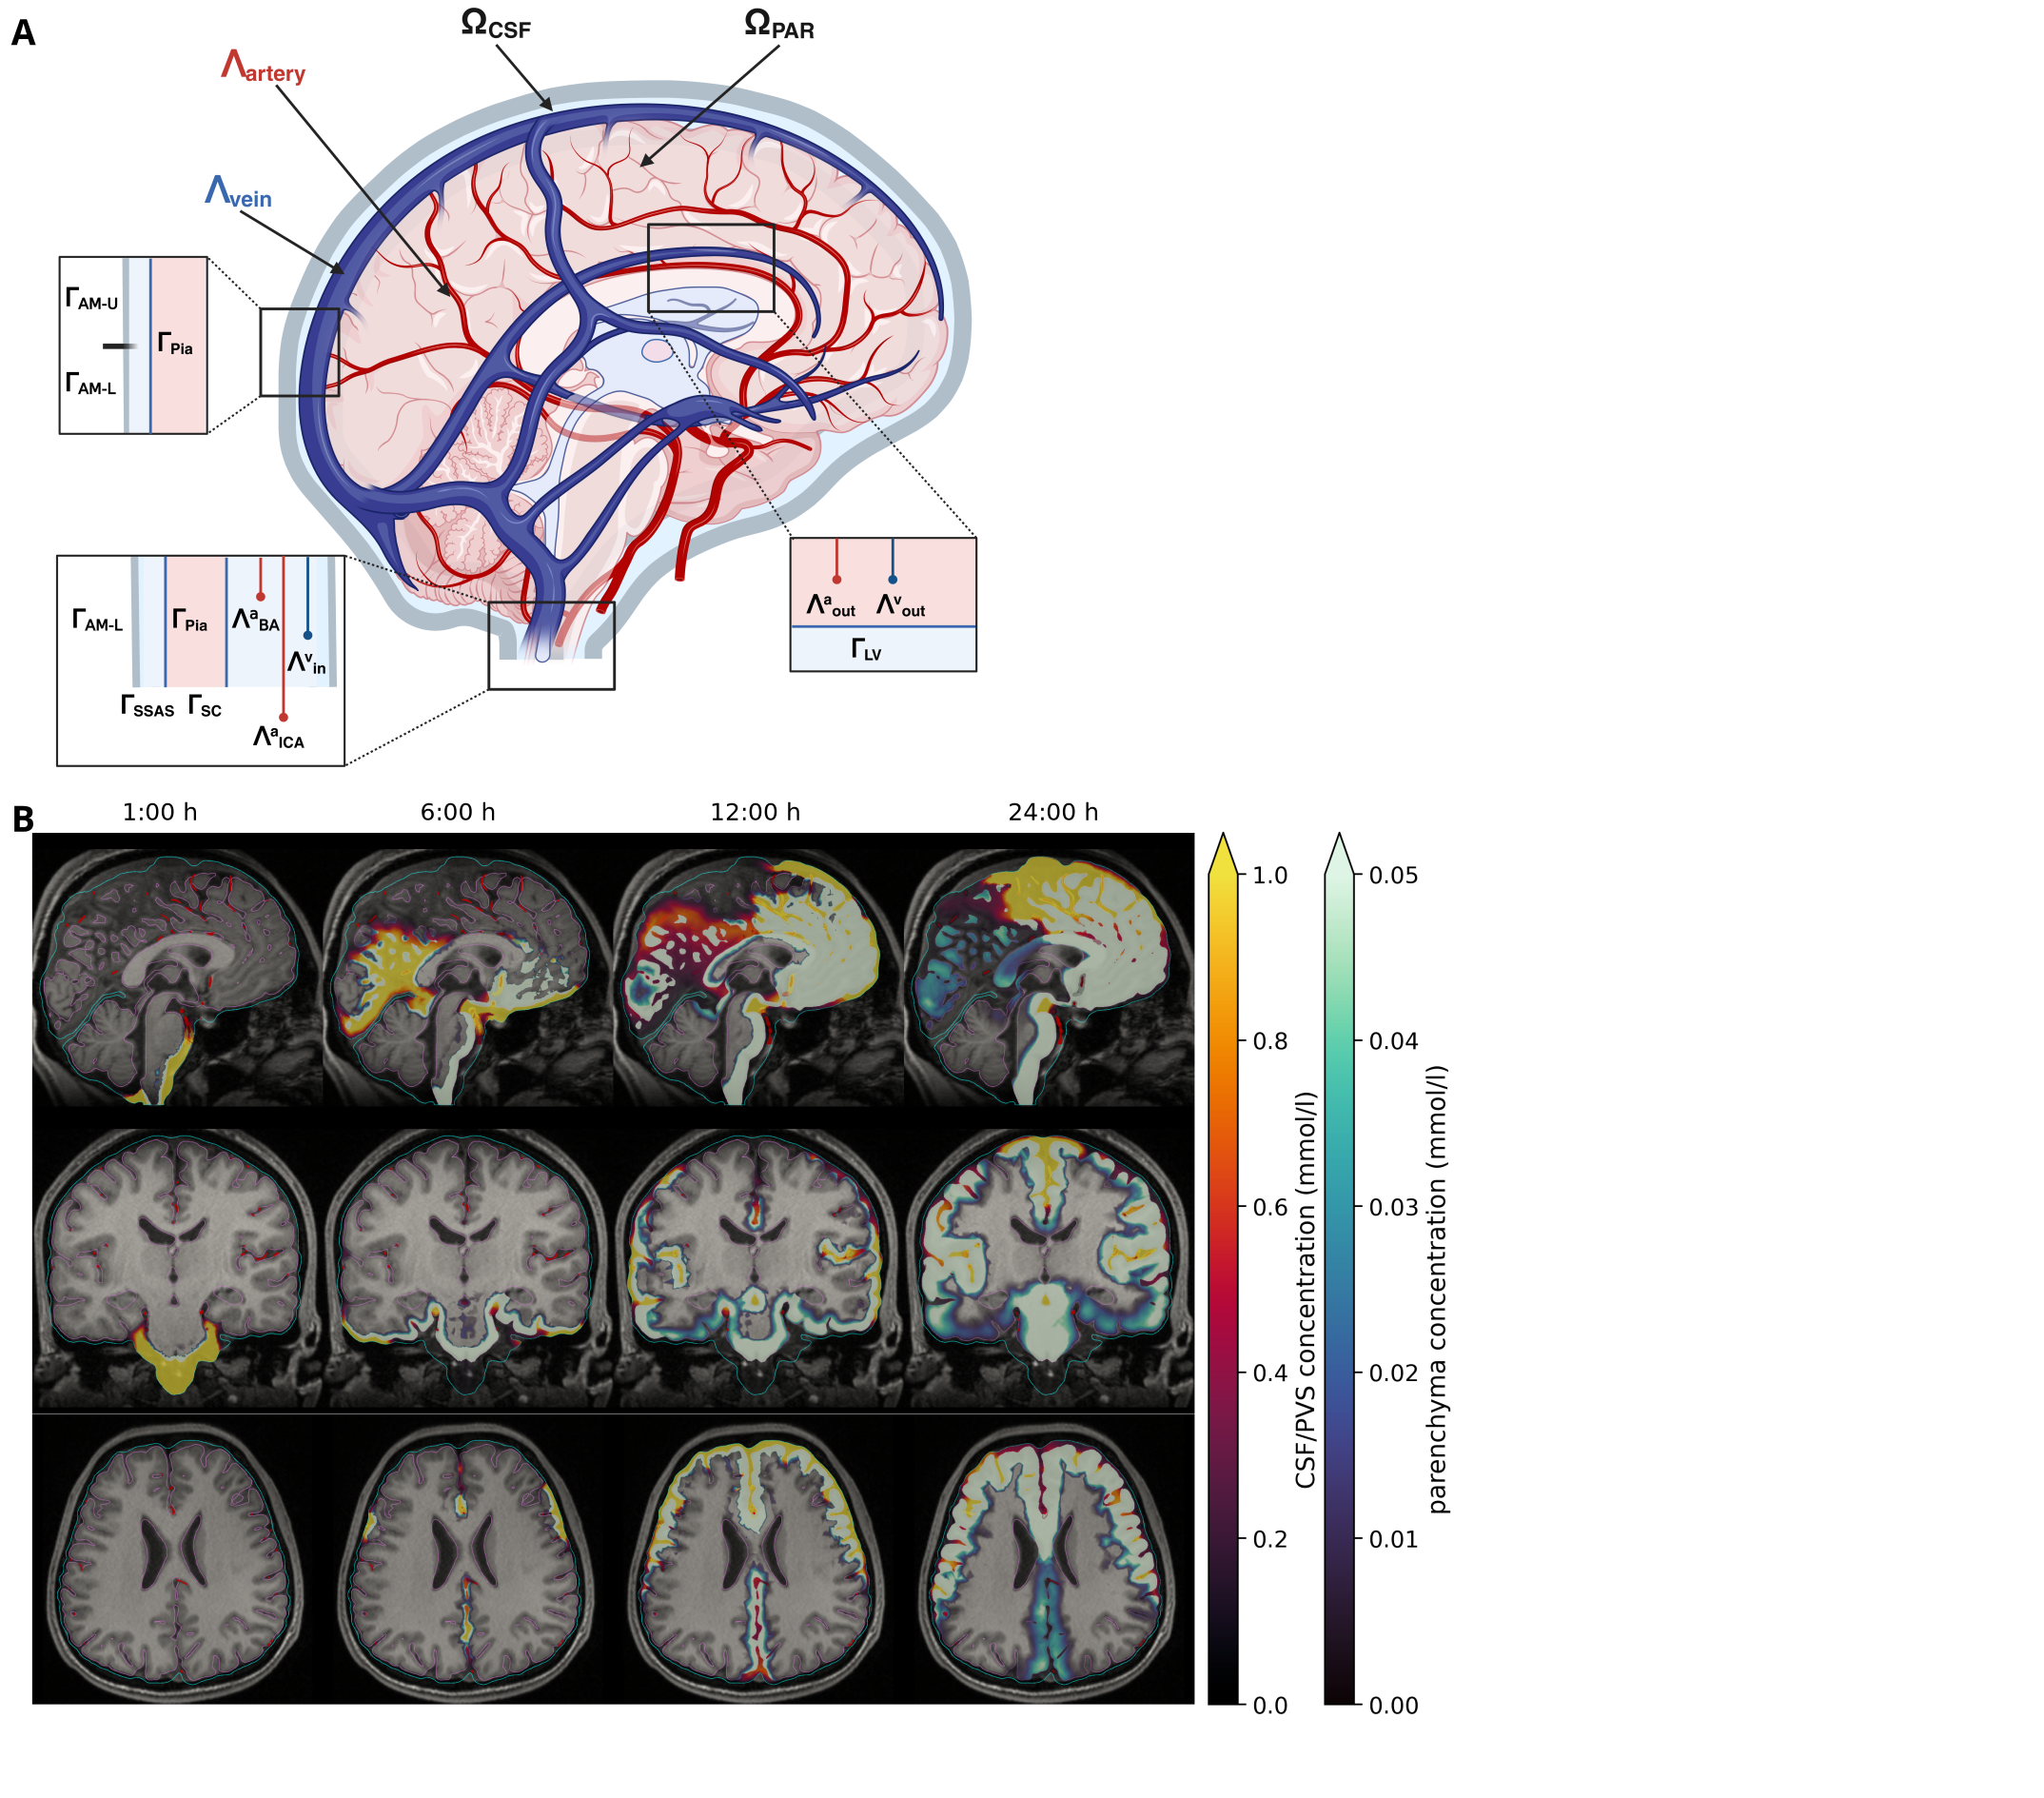
\includegraphics[width=1\textwidth]{figures/figure1.png}
     \caption{
     \textbf{In-silico modelling of tracer transport in the PVS, SAS and parenchyma.}
     A) Illustration of the model geometry including the CSF-filled spaces (ventricles and SAS) $\Omega_{\rm CSF}$, the parenchyma $\Omega_{\rm PAR}$ and the PVS surrounding arteries $\Lambda_{\rm artery}$ and veins $\Lambda_{\rm vein}$, as well as their interfaces and boundaries; 
     B) 3D rendering of the computational geometry: the parenchyma, CSF (clipped, blue), arterial network (red), and venous network (blue); 
     C) illustration of the intrathecal tracer injection protocol;  
     D) in-silico predictions of tracer concentration after 1, 6, 12, and 24 hours (opacity increasing linearly from 0 to 2 mmol/l); 
     E) sagittal, coronal and axial view of in-silico tracer concentrations overlayed on T1-weighted MR image after 1, 6, 12 and 24\,h (low concentrations transparent, pial surface in pink, arachnoid membrane in cyan, and arteries in dark red); 
     F) average tracer concentration in each compartment over the first 24\,h; 
     G) total amount of tracer in each compartment over the first 24\,h.}
     \label{fig:results1}
\end{figure}
Using previously published multi-modal magnetic resonance imaging
(MRI) data~\cite{hodneland2019new, deistung2009tof,
  schweser2012quantitative, reichenbach2012future,
  deistung2017overview}, we construct a multiscale computational
representation of the human intracranial compartments consisting of
the CSF spaces and brain parenchyma as three-dimensional (3D) domains
and with the PVSs surrounding major surface arteries and veins as
embedded networks of topologically one-dimensional (1D) curves
(\Cref{fig:results1}A--B). We consider a solute concentration field,
varying in space and time, in the 3D domains and in the PVS networks,
and assume that the solute can cross between these compartments
through semi-permeable membranes. As the drivers and modes of
intracranial transport are under substantial
debate\cite{smith2019going, proulx2021cerebrospinal,
  bohr2022glymphatic, hladky2022glymphatic, betsholtz2024advances},
our first target is to establish a baseline model accounting for a
reasonably conservative set of mechanisms and their integrated effect
over a timescale of several minutes to a few days. To this end, we
assume that the solute will (i) diffuse within all compartments, with
diffusivity depending on the effective properties of the relevant
medium\cite{sykova2008diffusion}; (ii) experience significant
dispersive effects due to the pulsatile flow of CSF induced by the
cardiac and respiratory cycles\cite{vinje2019respiratory,
  sharp2019dispersion, ray2021quantitative, troyetsky2021dispersion};
and (iii) be convected by a (small) net flow of CSF resulting from
production in the choroid plexus with CSF efflux across the upper
convexity\cite{hornkjol2022csf} and from the peristaltic pumping
effect of pulse wave pulsations in surface periarterial
spaces~\cite{mestre2018flow, gjerde2023directional}. Mathematically, this model is represented by a
mixed-dimensional system of coupled time-dependent partial
differential equations\cite{masri2024modelling}, which we solve
numerically with high accuracy using a mass-conserving finite element
scheme and the FEniCS finite element software\cite{alnaes2015fenics,
  kuchta2020assembly} (see Methods). The computational framework and
associated software are all openly available~\cite{ZENODO}.

Simulating a glymphatic MRI protocol~\cite{ringstad2017glymphatic,
ringstad2018brain, eide2024functional}(\Cref{fig:results1}C), we then predict the spreading of $0.5$ mmol intrathecally injected Gadobutrol after its appearance at the craniocervical junction, represented by tracer inflow across the spinal SAS boundary over the first two hours (\Cref{fig:results1}D--E). 
After one hour, the in-silico
tracer moves upwards in the SAS frontally of the brainstem, and
quickly reaches the supratentorial regions. Here, it spreads both
posterior through the quadrigeminal cistern and the longitudinal
fissure, and anteriorly through the outer SAS, reaching the top of the
cerebral cortex after around 12 hours. After 24 hours, the tracer
covers most of the brain surface (with the exception of some posterior
regions) and has penetrated substantially into the parenchymal
tissue. This pattern is reflected in the mean tracer concentrations in
each compartment, where the CSF space reaches its peak of
$1.4\,$mmol/l after 2 hours, followed by the arterial PVS
concentration peak ($2.9\,$mmol/l after 4 hours)
(\Cref{fig:results1}F). While the mean concentrations in these
compartments drop soon after peaking, the parenchymal tissue
slowly enriches with tracer over the first 24 hours, with a final
value of $0.3$ mmol/l. Overall, about 40\% of the total amount of
tracer remains in the cranium 24 hours post-injection, with the largest
share in the CSF (53\%), followed by the parenchyma (35\%), the
venous PVS (8\%) and the arterial PVS
(5\%) (\Cref{fig:results1}G).

\subsection*{Reduced CSF pulsatility strongly shifts intracranial enrichment patterns}
\begin{figure}%[h!]
\centering 
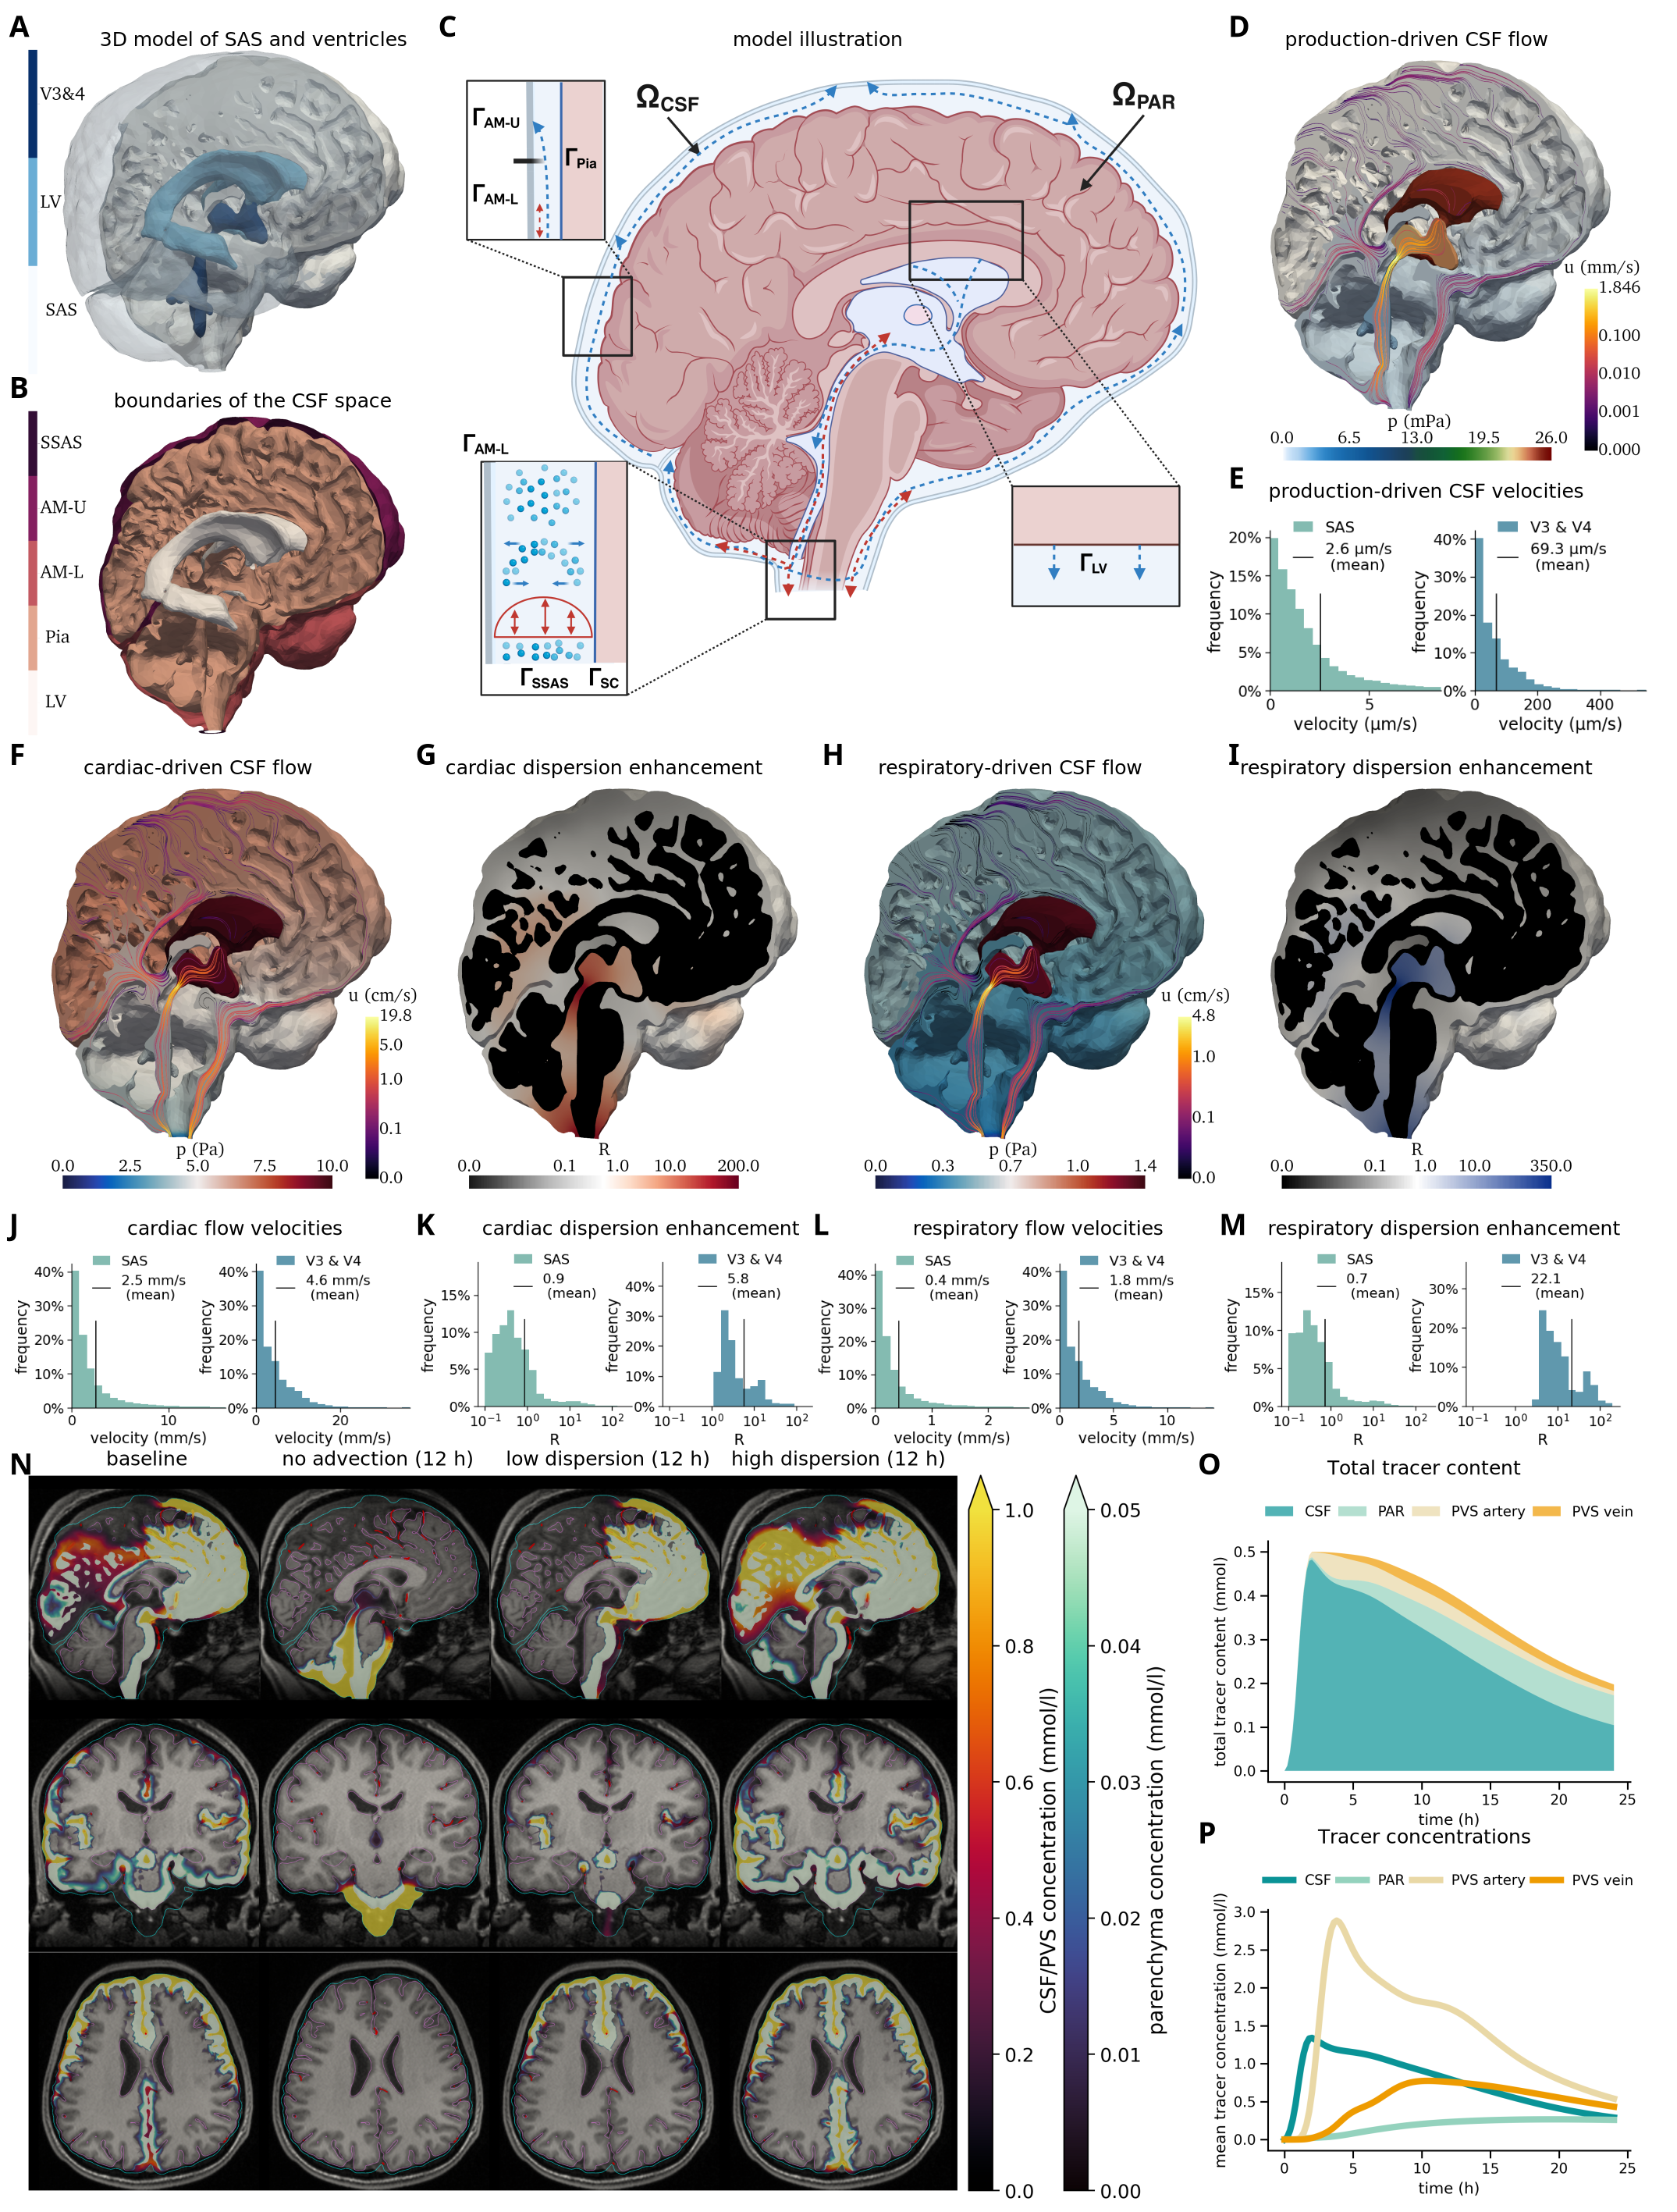
\includegraphics[width = 0.95\textwidth]{figures/figure2.png}
\caption{\textbf{The balance between CSF pulsatility and production shapes tracer enrichment patterns.}
A) CSF spaces: the third and fourth ventricle (V3\&4), lateral ventricles (LV) and SAS; 
B) Boundaries and interfaces: the spinal subarachnoid space (SSAS), upper and lower arachnoid membrane (AM-U and AM-L), pia (Pia) and lateral ventricles (LV); 
C) Schematic of the CSF flow model; 
D) CSF flow induced by CSF production with outflow allowed across the
upper convexity (AM-U); 
}
\label{fig:csf}
\end{figure}
\begin{figure}
\ContinuedFloat
\caption{(\textbf{cont.})
E) Histograms of the production-induced CSF velocities in the SAS and third and fourth ventricle (V3 \& V4) in terms of the relative frequency of the mean flow speed in each computational cell weighted by its volume; 
F) CSF flow induced at peak systolic blood inflow; 
G) Cardiac-induced dispersion factor $R_c$;
H) CSF flow induced at peak respiratory expansion; 
I) Respiration-induced dispersion factor $R_r$, $D = (1 + R_c + R_r) D^{\rm Gad}$; J--M): Histograms of the cardiac-induced flow velocities (J),
cardiac-induced dispersion factors (K),
respiratory flow velocities (L), respiratory dispersion factor (M);
N--Q): sagittal, coronal and axial planes of tracer concentration after 12h for different model variations: baseline (N), no CSF production (O), low dispersion (P), and high dispersion (Q).
}
\end{figure}  

The tracer enrichment patterns observed clinically after intrathecal
injection of contrast differ substantially between subjects and
between pathological conditions~\cite{ringstad2018brain,
  eide2021direction, eide2021impaired, eide2022altered}. These
neurological conditions are also associated with alterations in the
pulsatile flow of CSF in the ventricular system and
SAS~\cite{eide2021direction}. Clearly, key physiological factors such
as cardiac pulsatility and respiration easily differ between
individuals and between both pathological and physiological states. We
therefore next asked to what extent -- and how -- variations in CSF
pulsatility would affect the intracranial enrichment characteristics.

For the CSF dynamics in our baseline model, we combine the net
contribution to CSF flow induced by CSF production with the integrated
dispersive effects of cardiac and respiratory pulsatile CSF flow
(\Cref{fig:csf}A--C). Beginning with the advective, net flow field driven by 
CSF production, we impose a constant CSF inflow of $400\,$ml/day across the surface
of the lateral ventricles. Simultaneously allowing for efflux across the upper 
convexity yields a total CSF pressure drop of $26\,$mPa (0.00020 mmHg) (\Cref{fig:csf}D) with a
maximum flow velocity of $1.85\,$mm/s (in the aqueduct) and a mean
velocity in the SAS of $2.6$\textmu m/s (\Cref{fig:csf}E). Next, to examine the
dispersive effects of pulsatile CSF flow, we employ the theory of
shear-augmented dispersion together with computational fluid dynamics
to determine a dispersion factor $R$ enhancing the effective solute
diffusivity (see Supplementary information S1.3 for a complete description). 
To estimate the cardiac contribution, we compute the steady state
CSF pressure and flow fields at peak systolic blood inflow.
Modelling the reduction in CSF space volume corresponding to peak systolic
conditions, we assume a total inflow rate of $6\,$ml/s~\cite{baledent2014imaging, causemann2022human}
in the SAS across its outer surface and $0.31\,$ml/s 
across the lateral ventricle surface\cite{vinje2019respiratory}. 
This scenario sets up a pressure
drop of $10\,$Pa ($0.075$ mmHg) between the lateral ventricles and the
spinal SAS and a maximum flow velocity of $19.8\,$cm/s
(\Cref{fig:csf}F, J). Assuming a cardiac frequency of $1\,$Hz, we
infer that this cardiac-induced pulsatile CSF flow increases the
effective diffusion by more than two orders of magnitude in the
aqueduct and near the cisterna magna, but has little effect ($R <
1$) in most of the SAS (\Cref{fig:csf}G, K). For the respiratory
contribution, we employ the same methodology, but with a total rate of
$1\,$ml/s \cite{gutierrez2022effect} in the SAS and $0.121\,$ml/s
\cite{liu2024using} in the lateral ventricles, yielding a respiratory
peak flow volume of $1.121\,$ ml/s at the craniocervical
junction. While the resulting flow velocities are only about one
fourth of their cardiac-induced counterparts (\Cref{fig:csf}H, L),
respiratory dispersive mixing reaches a factor of up to 320 due the
lower respiratory frequency of $0.25\,$Hz (\Cref{fig:csf}I, M).

Now, to examine how CSF pulsatility affects the tracer enrichment patterns,
we consider three variations of the baseline: (i) no CSF production,
(ii) reduced pulsatility and thus decreased dispersion, and (iii) higher pulsatility with increased dispersion. We computed the reduced and increased pulsatility scenarios by halving and doubling the inflow rates associated with both cardiac and respiratory pulsations, which changed the dispersion factors by 0.25$\times$ and 4$\times$, respectively. Note that behaviour directly reflects the nature of our model: Stokes flow is linear in its inflow boundary conditions, and the diffusion enhancement factor is quadratic in the predicted pressure gradient.
Without CSF production, transport is considerably delayed
(\Cref{fig:csf}N, O). Even after $12$ hours, tracer remains in the
subtentorial regions around the cerebellum, the brain stem and in the
surrounding CSF. Interestingly, the lack of CSF production instead
allows tracer to travel upwards through the ventricular system,
reaching the third ventricle after around $12$ hours. On the other
hand, if the CSF pulsatility is reduced, we observe rapid transport
towards the upper convexity of the cranium, as in the baseline model,
but the tracer spreads exclusively within the anterior regions
(\Cref{fig:csf}P). This feature can be attributed to the CSF flow
bifurcation posterior to the ambient cistern (\Cref{fig:csf}D):
without sufficient diffusion, the tracer is unable to cross into the
posterior SAS. Indeed, with higher dispersion, the tracer moves
through the quadrigeminal cistern and further upwards into the
longitudinal fissure, with also enrichment of the cerebellum
(\Cref{fig:csf}Q).

\subsection*{Perivascular flow shapes and accelerates molecular transport}
\label{sec:pvs_flow_results}

The PVSs are recognized across species as critical pathways for solute
transport in and around the brain, and thus as potential targets for
enhancing brain drug delivery and metabolic waste clearance. However,
whether CSF flows more rapidly in PVSs and what the forces and
mechanisms required to drive such flow are, remain as key points of
debate~\cite{bohr2022glymphatic, van2024caa}. Motivated by
experimental observations in animal
models~\cite{iliff2012paravascular, iliff2013cerebral, mestre2018flow,
  bedussi2018paravascular}, there is now a remarkable body of
literature on modelling perivascular fluid flow and
transport~\cite{bilston2003arterial, asgari2016glymphatic,
  rey2018pulsatile, daversin2020mechanisms, sharp2019dispersion,
  thomas2019fluid, kedarasetti2020functional, kedarasetti2020arterial,
  troyetsky2021dispersion, martinac2021phase, gjerde2023directional,
  nozaleda2024arterial}. Here, we ask how these proposed mechanisms
would translate from idealized geometries to human vascular networks
and moreover, evaluate their integrated effect in the context of
intracranial solute transport.

Our periarterial network extends from the internal carotid arteries
and basilar artery through up to 18 bifurcations to reach upstream
network ends located within the SAS or up to 6 mm inside the
parenchyma (\Cref{fig:results1}A--B, \Cref{fig:pvs_a}A) and includes
major surface arteries of radius 0.5--1.4 mm. Due to imaging limitations, the network primarily covers the supratentorial regions, with the lowest network point located approximately $4\,$cm above the craniocervical junction.
Imposing the pressure field induced by CSF production at the periarterial network ends induces slow steady CSF flow of variable direction in these PVSs, with
an average velocity of 0.08 \textmu m/s (antegrade) and a maximum
velocity of 0.55 \textmu m/s (\Cref{fig:pvs_a}B). On the other hand,
traveling waves of arterial wall motion (\Cref{fig:pvs_a}C), such as
the pulse wave or other vasomotion~\cite{vanveluw2020vasomotion,
  munting2023spontaneous, bojarskaite2023sleep,
  broggini2024long,hauglund2025norepinephrine}, also induce net
directional flow in the PVS~\cite{kedarasetti2020arterial,
  kedarasetti2020functional, coenen2021lubrication,
  gjerde2023directional, nozaleda2024arterial} -- of magnitude and
direction depending on the amplitude, frequency, and length of the
waves and the characteristics of the perivascular
network~\cite{gjerde2023directional}. Applying a semi-analytic model
of the net flow induced by peristalsis in perivascular
networks~\cite{gjerde2023directional} (see Methods), we estimate that
the cardiac pulse wave alone, traveling at a frequency of 1 Hz with a
wavelength of 2.0 m and a 1\% wall displacement~\cite{jung2021novel},
will induce mainly antegrade PVS flow with an average net velocity of
0.92 \textmu m/s while reaching up to 7.31 \textmu m/s near larger,
ventral vessels such as the MCA (\Cref{fig:pvs_a}D,E). The same theory
predicts that strong ultraslow vasomotions, if traveling antegrade at
0.1Hz with a wavelength of 0.02 m and a 10\%
displacement~\cite{broggini2024long}, will induce both retrograde and
antegrade net PVS flow with an average velocity of 13.05 \textmu m/s
and maximum velocity 54.44 \textmu m/s (\Cref{fig:pvs_a}D,F).

We study the effect of such rapid PVS flow on intracranial molecular
transport by comparing the more conservative baseline model and a
high PVS flow model, where the former still includes the net flow
contributions from CSF production and the cardiac pulse wave, while
the latter additionally includes the ultraslow vasomotion
contribution. In both models, tracers were first observed at the basal
artery after 48 minutes (\Cref{fig:pvs_b}A), defined by their first-time arrival (FTA), the time at which the concentration first exceeds $0.1$ mmol/l. At all upstream locations along the middle cerebral arteries
(MCAs) and anterior cerebral artery (ACA), we found substantially
reduced FTAs with higher PVS flow (\Cref{fig:pvs_b}B), up to 2.5 hours
earlier in the left M2 segment of the MCA. PVS concentrations peaked
before the surrounding tissue (0:48h vs 1:12h at the MCA and 1:00h vs
1:48h at MCA2) with high PVS flow, while these peaks occurred nearly
simultaneously in the baseline model. The earlier appearance and the
delay in time-to-peak between the PVS and surrounding tissue clearly
indicates the directionality of tracer enrichment -- it first arrives
in the PVS and subsequently spreads into the tissue and SAS
(\Cref{fig:pvs_b}C, D), and especially so with higher PVS flow. These
observations also hold on an aggregated level: computing the total
amount of tracer in the PVS as a function of the distance to the
arterial network roots, we find accelerated tracer transport with
higher PVS flow, especially at earlier time points (2--9 hours)
(\Cref{fig:pvs_b}E). Moreover, differences in tracer transport along the
PVS translate to altered enrichment patterns on the whole-organ
scale. For instance, after 4-6 hours, the faster-moving tracer in the
PVS is clearly visible in the space adjacent to the PVS of the ACA, MCA, and other arteries (\Cref{fig:pvs_b}G). In contrast,
there are no clear signs of early enrichment surrounding the PVS in
the baseline model (\Cref{fig:pvs_b}F).

A natural question is whether early PVS enrichment could be the result
of increased dispersion rather than net flow in the
PVS\cite{asgari2016glymphatic,sharp2019dispersion,bojarskaite2023sleep,asgari2016glymphatic,troyetsky2021dispersion}. Interestingly,
even increasing the dispersion factor by $100 \times$ in the PVS,
induced only minor changes in the global spreading rate compared to the
baseline (\Cref{fig:pvs_b}F, H), thus indicating a negative answer to
this question.

\begin{figure}
    \centering
    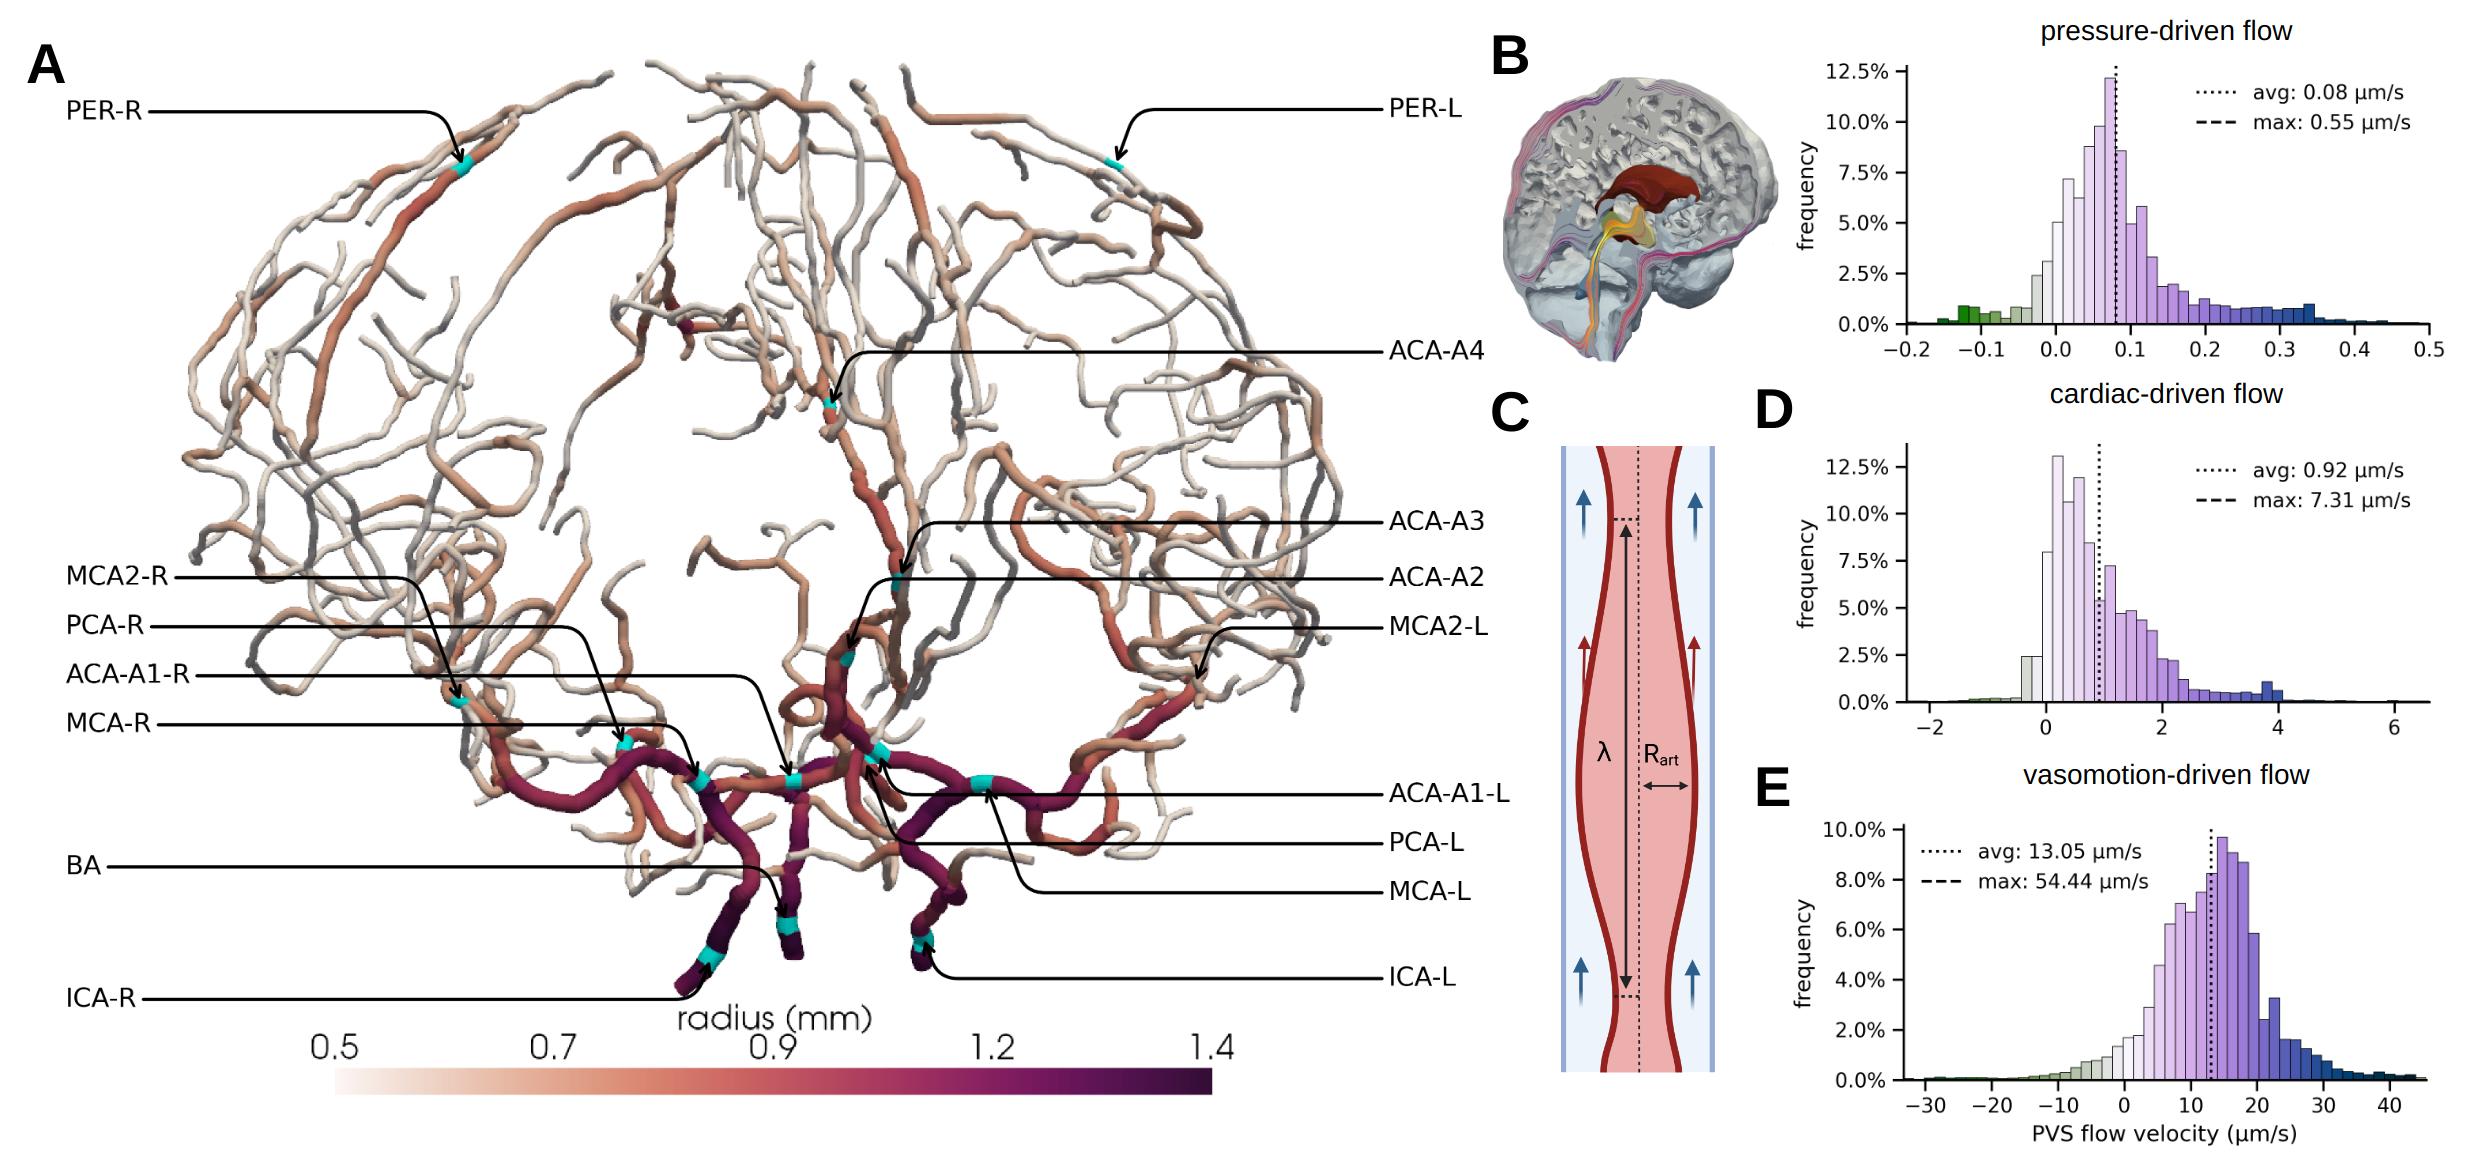
\includegraphics[width=0.95\textwidth]{figures/figure3a.png}
    \caption{\textbf{A static pressure gradient and peristaltic pumping are potential drivers of perivascular flow.}
    A) Surface arterial network colored by arterial radius with vessel locations labeled;
    B) Net PVS flow induced by CSF production alone (see also~\Cref{fig:csf}D).
    Histograms show the relative frequencies of local periarterial velocities. Positive values indicate antegrade PVS flow, while negative values indicate retrograde PVS flow;
    C) Illustration of the concept of peristaltic pumping;
    D) histograms of estimated net PVS flow induced by pulse wave or vasomotion peristaltic pumping;
    E) Estimated net PVS flow induced by pulse wave peristaltic pumping alone.
    F) Estimated net PVS flow induced by vasomotion/slow wave peristaltic pumping alone.}
    \label{fig:pvs_a}
\end{figure}
    
\begin{figure}
    \centering
    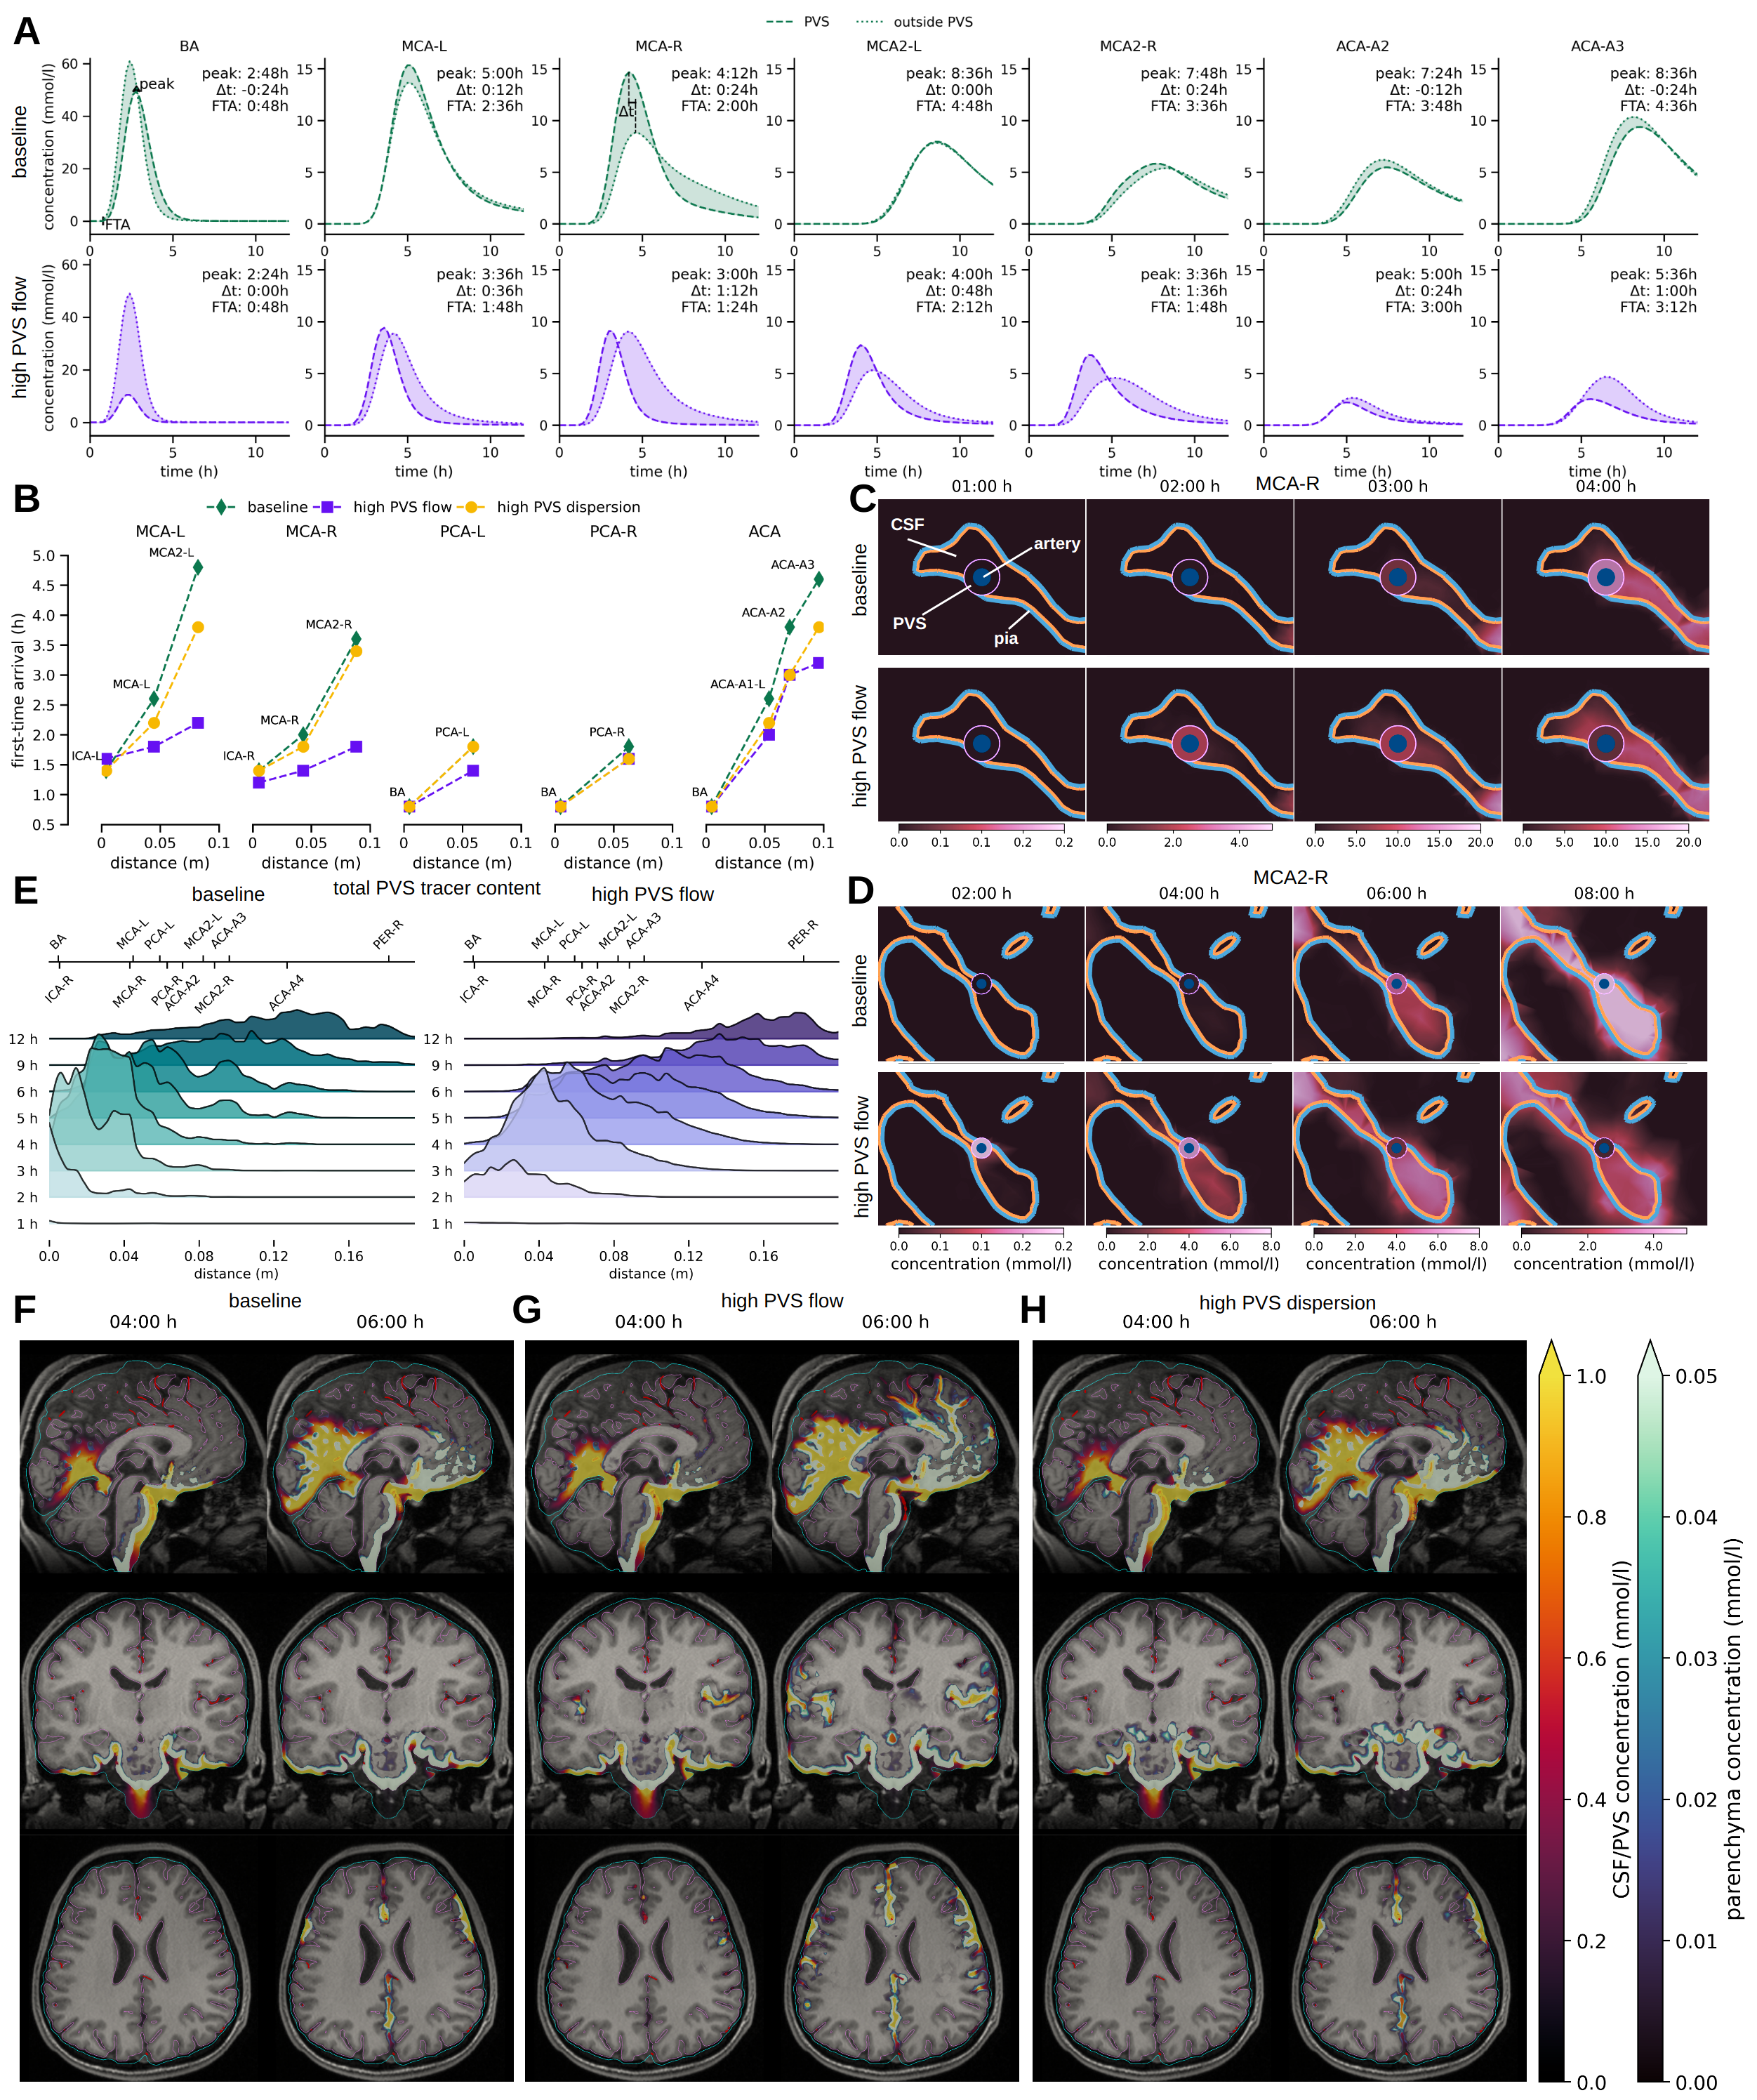
\includegraphics[width=0.99\textwidth]{figures/figure3b.png}
    \caption{\textbf{Perivascular flow shapes and accelerates molecular transport.}
    A) Comparison of mean tracer concentration in the PVS and over the outer PVS surface at key locations of the arterial tree, for the baseline (lower) and high PVS flow (upper) models, with labels: ``peak'': time-to-peak (h), ``$\Delta t$'': time difference between peaks (h), and ``FTA'': first-time tracer arrival (h).
    B) first-time arrival for the main trunks of the periarterial network over the distance from the closest network root node (BA, ICA-R or ICA-L for the baseline, the high PVS flow and the high PVS dispersion models);}
    \label{fig:pvs_b}
\end{figure}
\begin{figure}
\ContinuedFloat
\caption{(\textbf{cont.})
    C, D) 2D slices showing zoom-in on the region surrounding the MCA-R and MCA2-R for the baseline (upper) and high PVS flow (lower) models. Innermost circle indicates the artery (blue), the surrounding annulus is the PVS (color represents concentration value), the surroundings are parenchyma and/or CSF spaces, separated by the pia (blue: towards the parenchyma, pink: towards the CSF));  
    E) Total amount of tracer in the periarterial spaces as a function of the distance to the nearest network root over time for the baseline (left) and the high PVS flow (right) models;
    F--H) sagittal (upper) and coronal (lower) views of the simulated tracer concentrations overlayed on the T1-weighted MR image after 4 and 6h for the baseline (K), high PVS flow (L) and high PVS dispersion (M) models (concentration opacity linearly increasing with concentration value, pial surface outlined in pink, arachnoid membrane in cyan, and arteries in dark red). An interactive visualization of the baseline and the high PVS flow model can be found \href{https://baseline-pvs-flow.surge.sh/}{here}, and \href{https://high-pvs-flow.surge.sh/}{here}.}
\end{figure}  

\subsection*{Structural versus functional compartmentalization of perivascular spaces}

Human and rodent observations indicate that tracers concentrate in perivascular spaces surrounding the pial and subarachnoid vasculature \cite{zhang1990interrelationships,zhang1992directional, bedussi2017paravascular, mestre2018flow, bedussi2018paravascular, eide2024functional}. However, it remains unclear whether such enrichment patterns necessitate a structural barrier, such as a membrane with limited permeability, or if the patterns could result from enhanced flow or mixing in these areas alone. We therefore next investigate how the permeability of the interface between the PVS and the surrounding CSF affects tracer enrichment around the major arterial trunks (\Cref{fig:compartmentalization}A--B). To this end, we compare models with high and low  permeabilities, representing a highly permeable PVS-CSF interface (functional compartmentalization) and a less permeable interface (structural compartmentalization), respectively. For the low permeability model, we set the permeability to $3.8 \cdot 10^{-7}\,$m/s, consistent with previous estimates for the endfoot sheath surrounding penetrating arterioles \cite{koch2023estimates}, which we consider to be a lower bound for the surface PVS-CSF permeability. For the high permeability model, we increase this permeability by a factor of 100. We emphasize that, for both scenarios, we consider the high PVS flow regime as examined in the previous section. 

At the basal artery (BA), tracer appears within one hour in the surrounding CSF in both models (\Cref{fig:compartmentalization}C, E). With a more permeable PVS-CSF interface, tracer quickly crosses from the CSF into the PVS, resulting in similar peak concentrations of 25\,mmol/l in the PVS and at its outer surface, while values up to 50\,mmol/l are attained in the vicinity. In contrast, the low permeability model exhibits substantially lower perivascular tracer enrichment, with a maximum concentration of 10\,mmol/l after approximately two hours.
%The high permeability model allows for more tracer crossing into the PVS, leading to higher concentrations further downstream. Notably, crossover into the parenchyma is also observed, most clearly at 4 hours.
For the middle cerebral arteries (MCA-R and MCA-L), tracer appears
first in the PVS in both models (\Cref{fig:compartmentalization}D, E),
though with higher concentrations in the high permeability model (up
to 24 mmol/l). We also observe that the higher permeability allows the
tracer to leak out of the PVS and spread within the Sylvian fissure to
a greater extent. With a small delay, more tracer appears via
  the CSF pathway (\Cref{fig:compartmentalization}D). At the anterior cerebral artery (ACA-A2), the first tracer arrival in the PVS occurs after 3 hours, with a peak at 5 hours. The concentration peak in the PVS is tailed by a higher peak in the CSF (\Cref{fig:compartmentalization}E), indicating tracer arrival through a second pathway; i.e., directly through the CSF-filled space outside of the PVS. Similar patterns are observed for ACA-A3.

Summarizing and quantifying these observations
(\Cref{fig:compartmentalization}F), we find that neither the time of
first arrival nor the time-to-peak are substantially affected by the
PVS-CSF permeability at any of the periarterial segments considered
(BA, MCAs, ACAs). However, the concentration difference between the
PVS and its surrounding CSF quickly decreases with higher
permeability, as does the time lag between the concentration peaks in
these domains. Thus, fast transport along the PVS is not contingent
upon a structural compartmentalization of the PVS, whereas a sharp
concentration gradient between PVS and CSF is unlikely without a
restricting barrier.
\begin{figure}
    \centering
    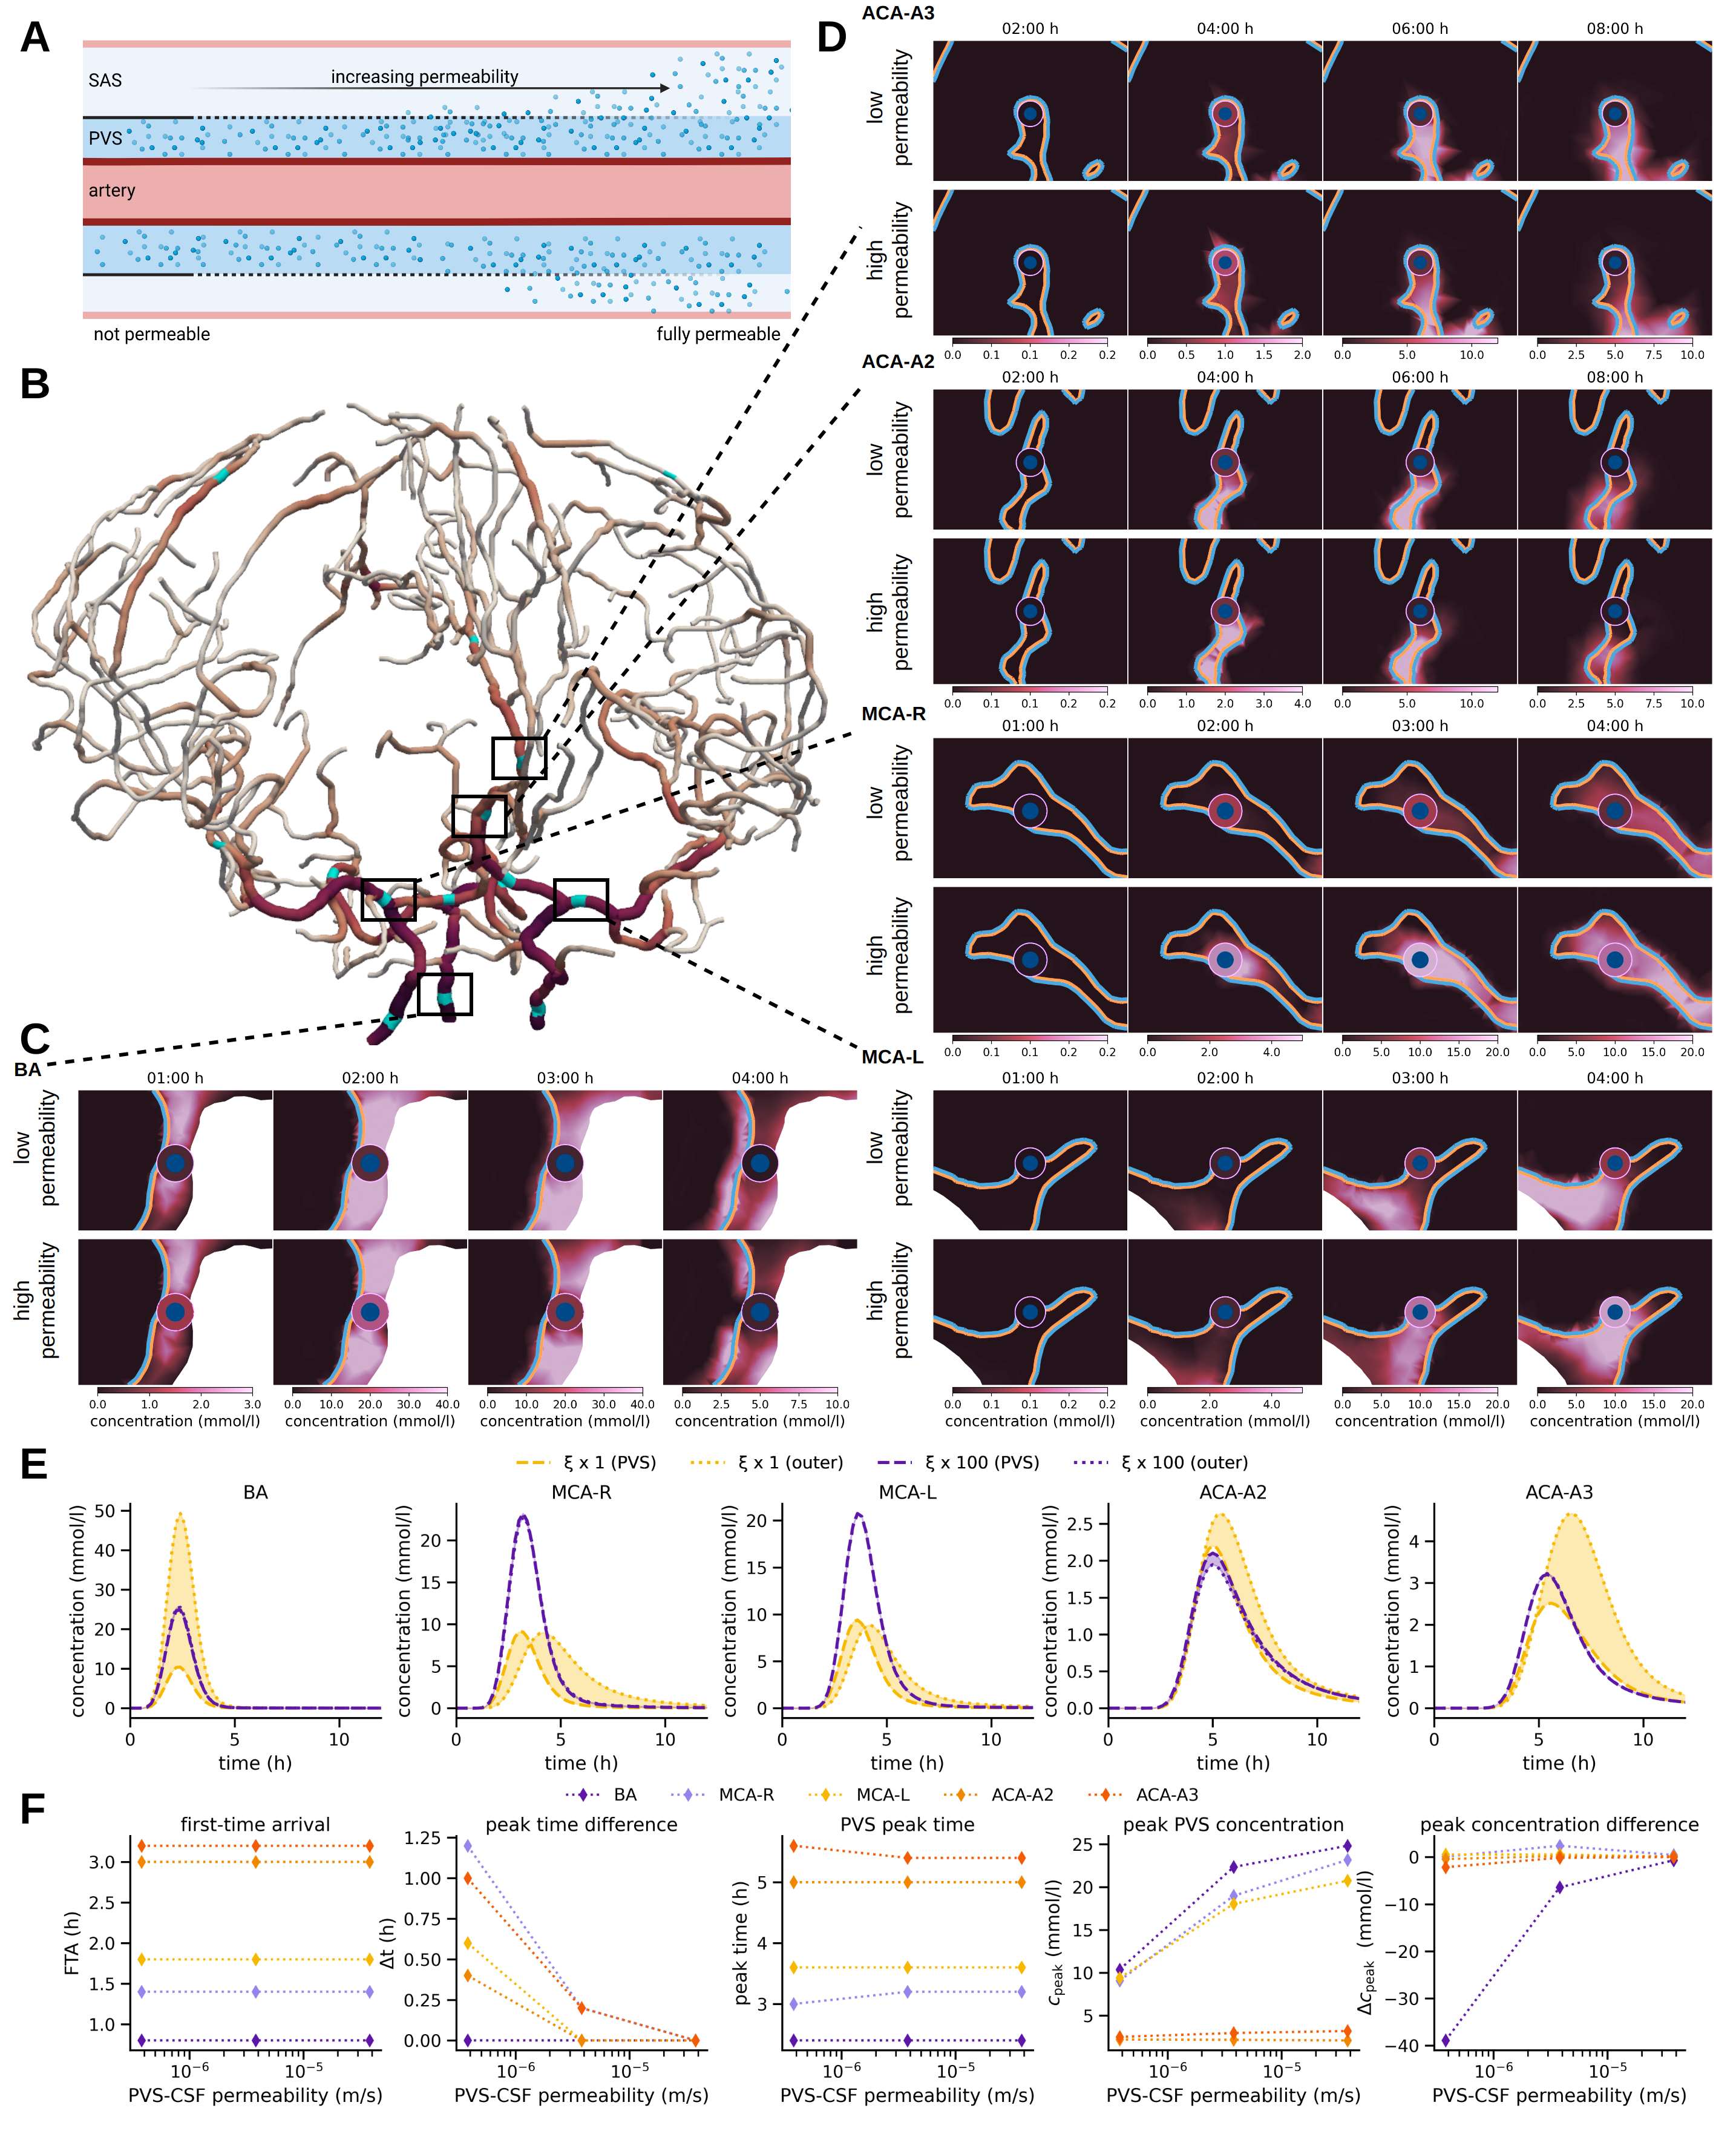
\includegraphics[width=0.95\textwidth]{figures/figure4.png}
    \caption{\textbf{Does early perivascular enrichment rely on a structural compartmentalization of the PVS?}
    A) The PVS-CSF membrane permeability regulates the exchange of solutes between the PVS and surrounding CSF spaces; 
    B) The arterial network with highlighted regions of interest; 
    C) 2D slices showing zoom-in to the region surrounding the basal artery after 1, 2, 3, and 4 hours for a low (above) and high (below) PVS-CSF permeability model. Innermost circle indicates the artery (blue), the surrounding annulus is the PVS (color represents concentration value), the surroundings are parenchyma and/or CSF spaces, separated by the pia (blue: towards the parenchyma, pink: towards the CSF). The cutting planes are normal to the blood vessels;
    D) As in (C) for regions surrounding (from upper to lower) the ACA-A3, ACA-A2, MCA-R and MCA-L segments;}
    \label{fig:compartmentalization}
\end{figure}
\begin{figure}
\ContinuedFloat
\caption{(\textbf{cont.})
E) Comparison of mean tracer concentration in the PVS (dashed) and over the
outer PVS surface (dotted) for the BA, MCA-R, MCA-L, ACA-2, and ACA3 segments over time for the high (purple) and low permeability (yellow) models;
F) Effect of varying the PVS-CSF permeability on first-time-of-arrival (FTA), time difference ($\Delta t$) between concentration peaks in the PVS and surrounding tissue, time of PVS peak concentration, PVS peak concentration and difference in peak concentration between PVS and surrounding tissue.}
\end{figure}
  
\subsection*{Enlarged PVSs in the SAS delay periarterial and intracranial tracer enrichment}

Idiopathic normal pressure hydrocephalus (iNPH), a dementia subtype,
is associated with enlarged PVS in the SAS and impaired periarterial
and parenchymal tracer transport~\cite{eide2024functional}. More
generally, enlarged PVSs are associated with a range of pathophysiogical
conditions and cognitive decline~\cite{bown2022physiology}. A key
question is thus whether enlarged PVSs alone leads to delayed
perivascular and intracranial tracer enrichment. To address this
question from a fluid and transport dynamics perspective, we ask our
in-silico model to predict the integrated effect of perivascular
dilation on PVS flow velocities and tracer enrichment patterns
(\Cref{fig:enlargement}A).

Again we compute CSF production-, cardiac-, and vasomotion-induced net PVS flow velocities, but now in a perivascular geometry with an increased outer radius ($R^{\rm dilated}_2 = 3 R_1$) compared to the previous ($R^{\rm control}_2 = 2 R_1$), which corresponds to a $2.67 \times$ increase in PVS cross-section area.
%% \begin{align*}
%%   A_1 = \pi (R_2^2 - R_1^2) = \pi (2^2 R_1^2 - R_1^2) = 3 \pi R_1^2 \\
%%   A_2 = \pi (\hat{R}_2^2 - R_1^2) = \pi (3^2 R_1^2 - R_1^2) = 8 \pi R_1^2 \\
%%   A_2 / A_1 = 8/3 = 2.76
%% \end{align*}
The enlargement yields notable and non-uniform changes in the flow
dynamics. On the one hand, the pressure-induced flow velocities
increase from a mean of 0.08 \textmu m/s to 0.33 \textmu m/s due to
the reduced effective resistance of the PVS. However, the peristaltic
pumping becomes considerably less effective: the cardiac and
vasomotion-induced net CSF flow velocities drop from a mean of 0.92
\textmu m/s to 0.17 \textmu m/s and from 13.05 \textmu m/s to 2.33
\textmu m/s, respectively (\Cref{fig:enlargement}B--D). In total, the
net CSF velocity reduces, which in turn alters the tracer enrichment
within the dilated PVS. Notably, we observe later tracer arrival in
all MCA segments, with up to 96 min later arrival in the
MCA2s for the high PVS flow scenario (\Cref{fig:enlargement}E, F). For
the baseline model, which omits the vasomotion-induced net PVS flow,
the effect is less pronounced in the MCA but clearly persists and is
evident in the MCA2s (\Cref{fig:enlargement}F). Finally, we note that
the larger volume of the dilated PVS results in a greater total
accumulation of tracer in the PVS from 3--24 hours and reduced
enrichment of the parenchyma at 6 and 12 h, while the mean PVS
concentration is initially lower, but later exceeds the baseline model (\Cref{fig:enlargement}G,H).
\begin{figure}
    \centering
    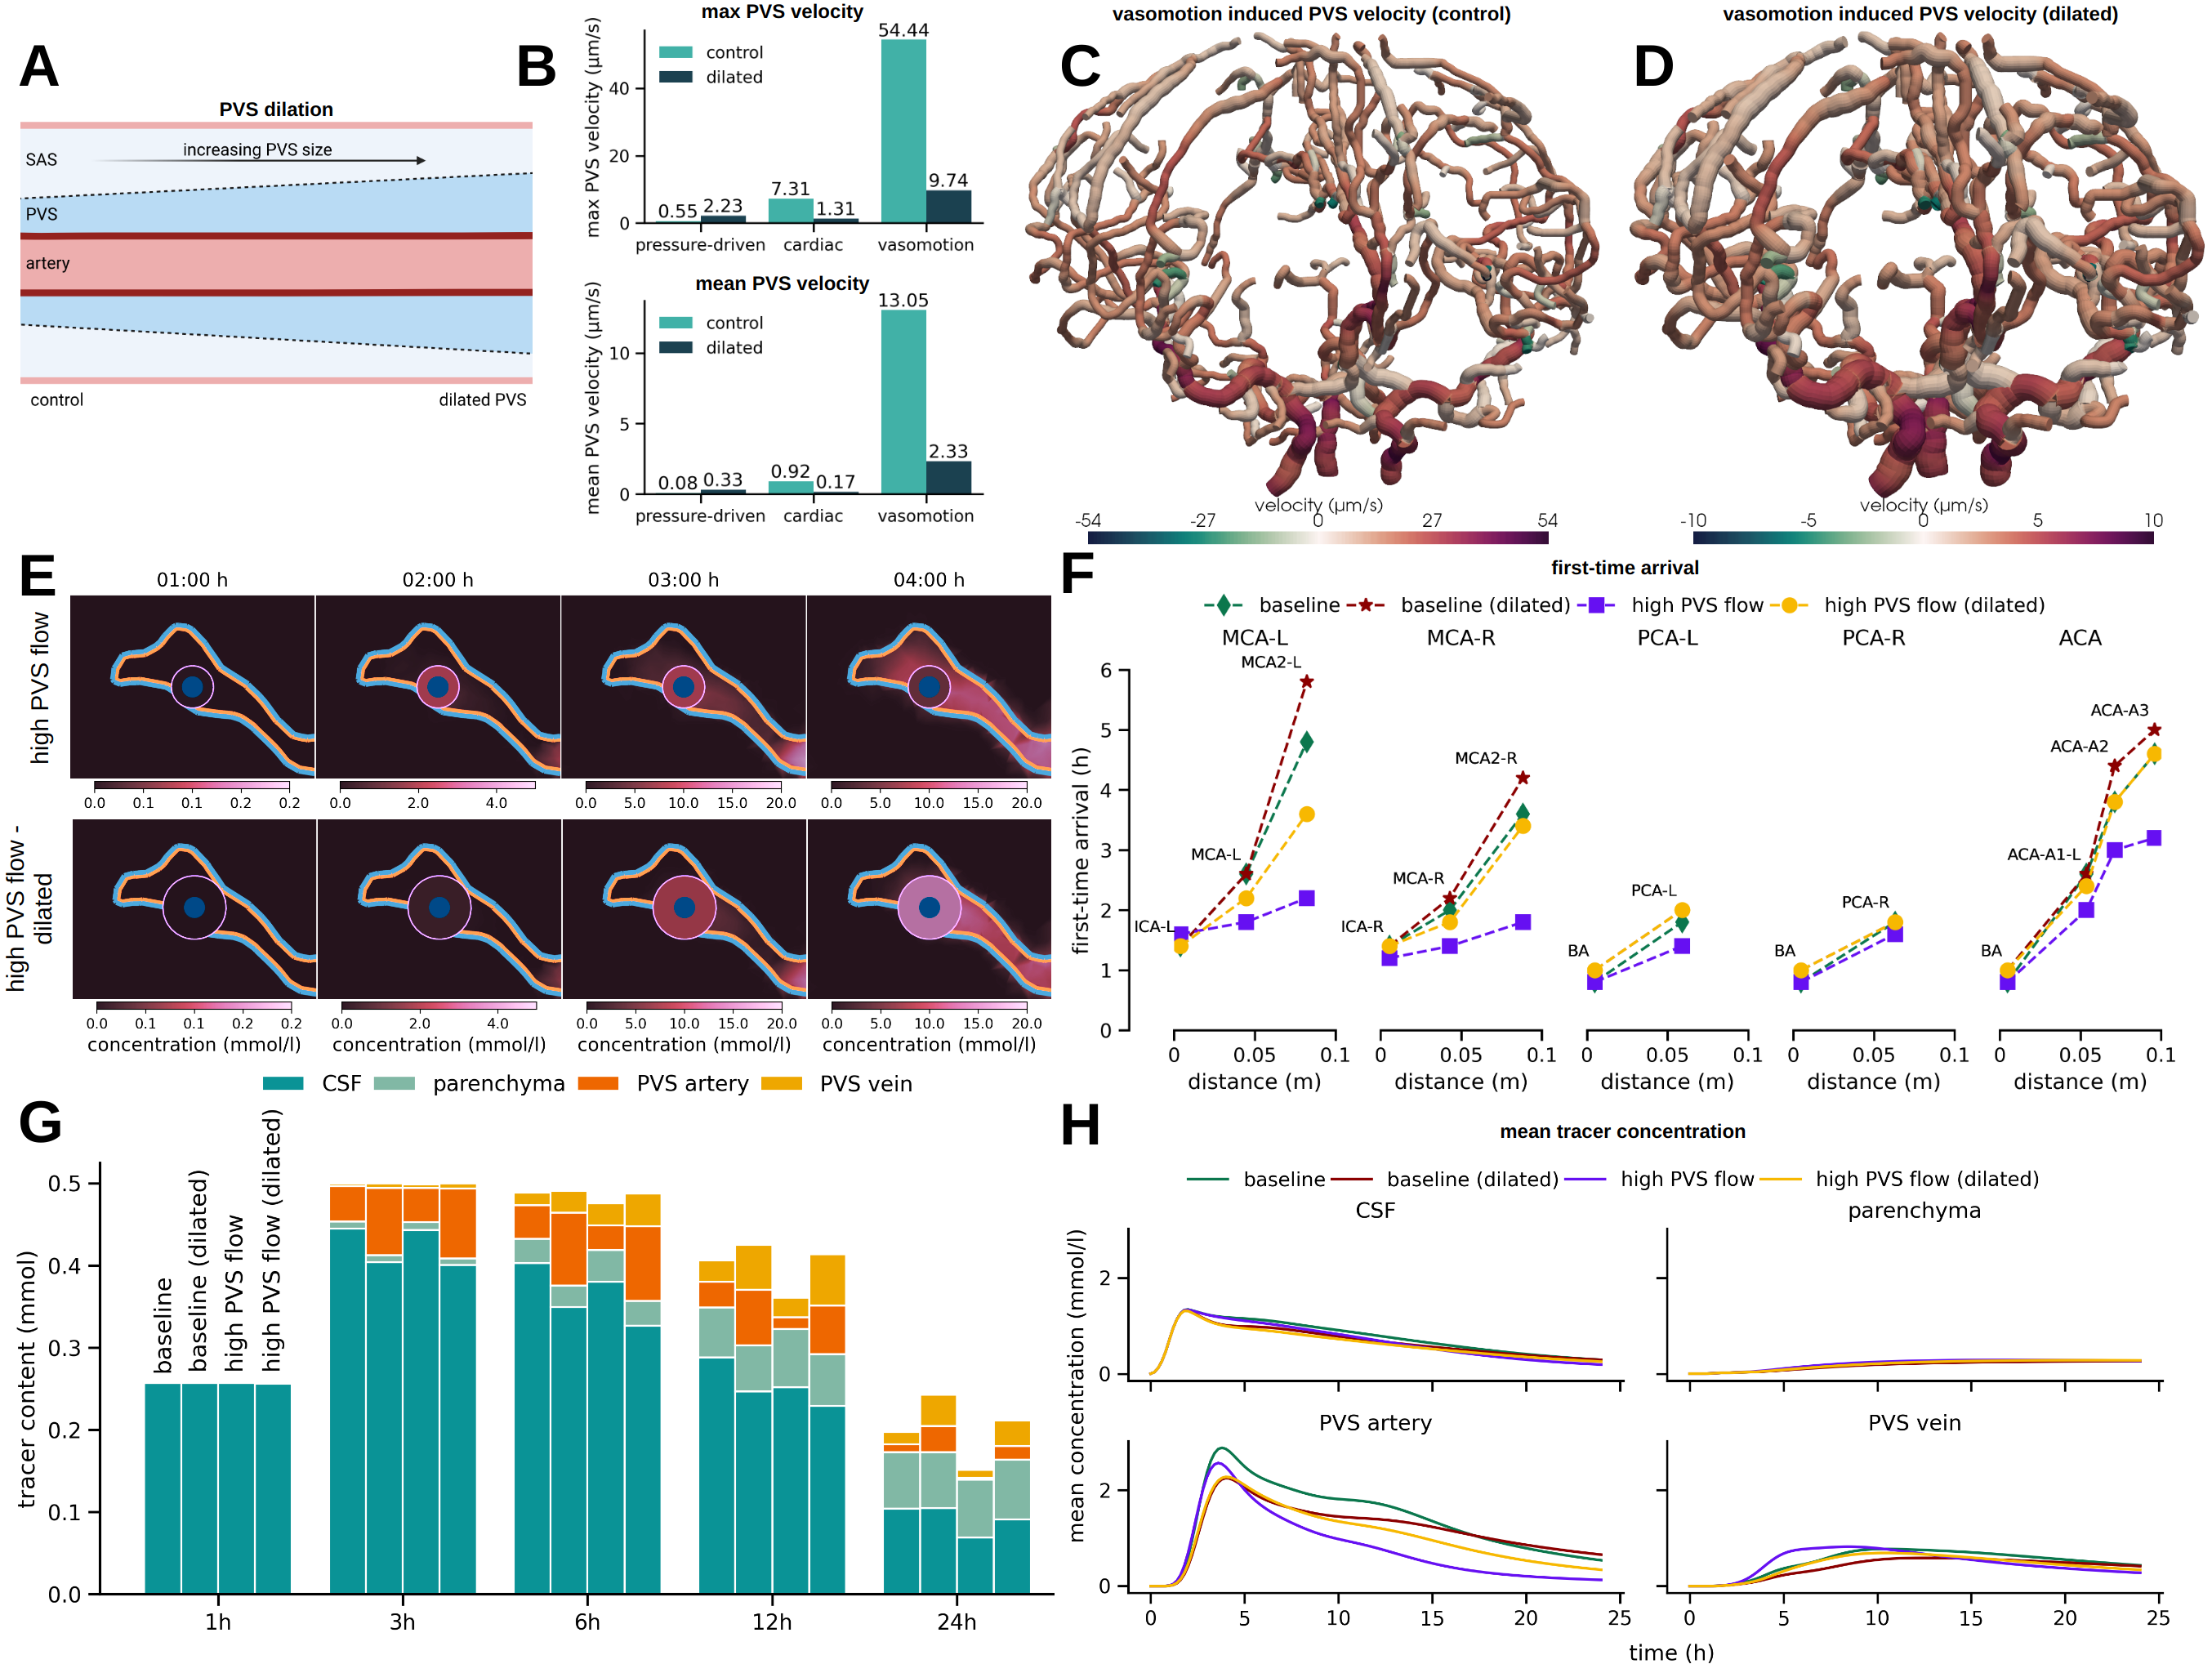
\includegraphics[width=1 \textwidth]{figures/figure5.png}
\caption{\textbf{PVS enlargement in the SAS reduces net PVS flow and delays tracer transport}
A) Modelling dilated PVS in the SAS by extending the outer PVS boundaries;
B) mean and max PVS flow velocities with normal/control and dilated PVS;
C--D) 3D rendering of vasomotion-induced PVS flow in the normal (C) and dilated (D) periarterial networks; 
E) 2D slices showing zoom-in to the region surrounding the MCA-R after 1, 2, 3, and 4\,h with normal (lower) and dilated (upper) PVS. Innermost circle indicates the artery (blue), the surrounding annulus is the PVS (color represents concentration value), the surroundings are parenchyma and/or CSF spaces, separated by the pia (blue: towards the parenchyma, pink: towards the CSF).The cutting plane is normal to the blood vessel; 
F) First-time arrival for different branches of the arterial tree for the baseline model (with pressure-driven and cardiac-induced net PVS flow) and the high PVS flow model (also including vasomotion-induced net PVS flow) for normal and dilated PVS;
G) total tracer content in the CSF, parenchyma and arterial and venous PVS at 1,3,6,12 and 24\,h for the four models from F;
H) mean concentration in the CSF, parenchyma and arterial and venous PVS over time for the four models from F.
}
    \label{fig:enlargement}
\end{figure}

\section*{Discussion}

%% Summary of findings
We have presented a high-fidelity in-silico model of molecular
enrichment and clearance in human intracranial spaces, enabling
tailored predictions of the influence of CSF space and (peri)vascular
morphology, physiological factors such as cardiac and respiratory
pulsatility, as well as of pathological conditions such as enlarged
PVSs in the SAS. A key observation is that the balance between CSF
production and intracranial pulsatility significantly shapes the
large-scale features of tracer enrichment, with e.g.~ventricular
tracer reflux after intrathecal injection in the absence of CSF
production, and preference towards anterior brain regions with reduced
pulsatility. Indeed, the simulated distribution patterns cover a
substantial range of the individual variations observed clinically
\cite{ringstad2018brain}. In terms of perivascular pathways, we find
that even moderate CSF flow on the order of 0.1--1.0 \textmu m/s in
the surface PVSs results in earlier tracer enrichment around major
cerebral arteries. This effect is more pronounced -- with up to a
three-hour difference in time of arrival -- with mean PVS flow rates
of approximately 10 \textmu m/s. Our models of CSF flow in
perivascular networks, based on first principles and asymptotic
analysis, predict net flow of such magnitudes and both antegrade and
retrograde flow within the perivascular network. The PVS may thus
function as highways facilitating rapid transport, even in the absence
of structural barriers, though a sharp concentration difference
between the PVS and surrounding tissues is unlikely without such
barriers. Finally, dilated PVS in the SAS will cause a substantial reduction in
cardiac- and vasomotion-driven flow velocities, which in turn impedes
perivascular transport.

%% Comparison with others

% Tracer enrichment predictions
While tracer enrichment of the brain and surrounding CSF spaces
have been extensively studied in animal models, especially in murine
models in connection with studies of the glymphatic system, there are
fewer reports of contrast enrichment in human subjects over 0--24h. We
therefore mainly compare our in-silico predictions with the series of
papers by Eide and colleagues~\cite{ringstad2017glymphatic,
  ringstad2018brain, eide2021sleep, eide2024functional} and Watts et
al~\cite{watts2019measuring}. Ringstad et al.~\cite{ringstad2018brain}
report of tracer enrichment in a centripetal pattern, primarily in
regions near large cerebral surface arteries, peaking in the CSF
spaces between 6 and 9 hours, with parenchymal tracer content still
increasing after 24 hours, but with large individual
differences. Watts et al~\cite{watts2019measuring} report of a similar
enrichment pattern and a concentration peak in the SAS of $\approx$0.5
mmol/l (relative to a total amount of 1.0 mmol) occuring after 10 to 15 hours. 
Our in-silico enrichment patterns agree with these observations, though with an earlier rather than later peak in the CSF spaces (2 hours after first tracer appearance at the craniocervical junction). In particular, we note that the substantial individual variation observed clinically is comparable to the variation in in-silico enrichment patterns associated with reduced CSF production or reduced intracranial pulsatility. We find that about 20\% of the tracer reaching the cranium enters the parenchyma, which aligns with the reported peak concentration values of $0.5\,$mmol/l in the SAS and $0.1\,$mmol/l in the parenchyma reported by Watts et al~\cite{watts2019measuring}.

Importantly, our simulation results indicate that the tracer
enrichment observed clinically relies on the presence of one or more
flow drivers in addition to CSF production and cardiac
peristalsis. Dispersion due to cardiac and respiratory pulsations has
been hypothesized to enhance transport in the perivascular spaces as
well as in the CSF spaces. However, recent estimates indicate that the
effect of dispersion in the PVS does not exceed a factor of 2 compared
to diffusion alone
\cite{asgari2016glymphatic,sharp2019dispersion,bojarskaite2023sleep,asgari2016glymphatic,troyetsky2021dispersion}. Our
model demonstrates that not even a 100-fold increase in the PVS
dispersion coefficient accelerates transport substantially
(\Cref{fig:pvs_b}H). To illustrate the need for a stronger advective
driver, we compared our findings to tracer arrival times reported by
Eide and Ringstad~\cite{eide2024functional}, who observed a delay of
just 15.3 min between the M1 and M2 segments of the MCA. First, we
note that the spaces studied by Eide and
Ringstad~\cite{eide2024functional}, labeled therein as the PVSAS, are
naturally compared to the parts of our surface PVS networks embedded
within the SAS. Our baseline model, accounting only for CSF production
and cardiac-driven flow, predicted a physiologically unrealistic delay
of over three hours. In contrast, our high PVS flow scenario, which
incorporates the effects of low-frequency vasomotion, yielded a more
consistent delay of 24 minutes. Furthermore, after adjusting for the
13 min travel time from injection to the craniocervical
junction~\cite{eide2024functional}, the high PVS flow model's FTAs
(84--108 min for M1) aligns well with the upper end of the reported
clinical range (37.8 $\pm$ 47.0), particularly when considering
potentially delayed transport due to the limited caudal extent of our
PVS network. All in all, we interpret these results as strongly
indicative of that PVS flow driven by CSF production and cardiac
peristalsis alone is insufficient to explain the rapid perivascular
transport observed in humans.

% PVS flow predictions. 
The existence, magnitude, and directionality of flow in surface and
parenchymal PVSs have been the subject of active debate for
decades~\cite{rennels1985evidence, bilston2003arterial,
  hadaczek2006perivascular, carare2008solutes, iliff2012paravascular,
  iliff2013cerebral, bakker2016lymphatic, mestre2018flow,
  bedussi2018paravascular, rey2018pulsatile, thomas2019fluid,
  daversin2020mechanisms, kedarasetti2020functional,
  martinac2021phase, vanveluw2020vasomotion, bohr2022glymphatic,
  boster2023artificial, gjerde2023directional,
  nozaleda2024arterial}. In mice, Mestre et al~\cite{mestre2018flow}
observe CSF flow in surface perivascular regions surrounding branches
of the MCA with average flow speeds of 18.7 \textmu m/s and net flow
in the antegrade direction, but also regions with retrograde
flow. Similarly, Bedussi et al.~\cite{bedussi2018paravascular} report
of oscillatory flow, with an average (net) CSF velocity of 17 $\pm$ 2
\textmu m/s in the antegrade direction. Using physics-informed neural
networks, Boster et al~\cite{boster2023artificial} estimate PVS
velocities of $12.75 \pm 6.25$ \textmu m/s. Less is known about the
magnitude and directionality of CSF flow in surface PVSs in
humans. Here, assuming that human surface PVS follow the major surface
vessels and are CSF-filled but otherwise open regions of width
proportional to the vessel radius, our estimates indicate that the CSF
pressure differences due to CSF production, cardiac peristaltic
pumping and low-frequency vasomotion all yield spatially-varying net
CSF flow with both antegrade and retrograde PVS segments. This
observation is thus in agreement with the experimental
observations~\cite{mestre2018flow, bedussi2018paravascular}, and
inherently supports the original notion that antegrade and retrograde
solute transport along PVSs may coexist~\cite{rennels1985evidence}. In
terms of magnitude, the contribution from CSF production and cardiac
wall motion are small (0.08 \textmu m/s and 0.92 \textmu m/s on
average), but intriguingly, our estimates of the contribution from
vasomotion (13.05 \textmu m/s) are comparable to the experimental
reports. We do note that this estimate is based on the presence of
rhythmic waves of vasomotion at a frequency of 0.1Hz, a wavelength of
20 mm, and a wall displacement of 10\% -- in the antegrade direction,
all values currently associated with major
uncertainty~\cite{gokina1996electrical, vanveluw2020vasomotion,
  munting2023spontaneous, broggini2024long}. In particular, Broggini
et al\cite{broggini2024long} report of near-0.1Hz vasomotion waves
traveling both antegrade and retrograde along pial arterioles in
mice, while Munting et al\cite{munting2023spontaneous} report of
vessel diameter changes at similar frequencies mainly (but not
entirely) in the retrograde direction. To the best of our knowledge,
less is known about vasomotion wave characteristics in the human
cerebral vasculature, though Gokina et al\cite{gokina1996electrical}
report of spontaneous vasomotion also in human pial arteries ex-vivo.


% Compartmentalization of the PVS
To what extent are surface PVSs in communication with the surrounding
SAS and to what extent are these structurally separated compartments?
Originally, Weller and coauthors~\cite{zhang1990interrelationships,
  zhang1992directional, weller2005microscopic} identified thin sheaths
of pial cells surrounding human surface arteries and penetrating
arterioles (but not veins or venules). On the other hand, Bakker and
coauthors report that the subarachnoid space, the cisterns, ventricles
and penetrating periarteriolar spaces form a continuous CSF
space~\cite{bedussi2017paravascular}. Thorne and colleagues study the
architectures of rat perivascular spaces in detail, emphasizing the
presence of openings (stomata) on the interface between the
vasculature and the CSF within the SAS~\cite{pizzo2018intrathecal,
  hannocks2018molecular}. Further, Mestre et
al~\cite{mestre2022periarteriolar} study the properties of pial
perivascular spaces in mice, and report of pial cells forming sheaths
for larger surface arteries and partially cover smaller surface
arteries, with higher coverage in ventral SAS regions. Our results
demonstrate that the PVSs may act as rapid transport pathways even
with only a partial barrier between the PVS and surrounding CSF, thus
contributing to quantifying the properties of the human PVS-CSF
interface~\cite{eide2024functional}. In this regard, we emphasize that
we report on the isolated effect of variations in permeability on
molecular transport, separated from any effects on fluid flow in the
PVS. Clearly, one may expect that the presence and/or properties of
such a barrier would affect also PVS flow. However, considering the
uncertainty associated with PVS flow characteristics in the human SAS
in general and the lack of computational models describing net PVS
flow in the presence of fluid exchange, this remains challenging to
quantify.

% Variations with sleep, exercise
Lifestyle factors such as sleep~\cite{xie2013sleep, miao2024brain,
  bojarskaite2023sleep, eide2021sleep, vinje2023human,
  hauglund2025norepinephrine, larsen2024sleep},
exercise~\cite{holstein2018voluntary, yildiz2022immediate}, and
alcohol intake~\cite{lundgaard2018beneficial} affect molecular
enrichment and clearance of the brain. In particular, pial arteries
display higher-amplitude low-frequency vasomotion during NREM and
intermediate sleep states, while REM sleep is associated with reduced
PVS width~\cite{bojarskaite2023sleep}. Peristaltic pumping is more
effective under both of these configurations, resulting in higher
estimated net PVS flow velocities~\cite{gjerde2023directional}. Even
higher PVS velocities would amplify the PVS flow effects simulated
here, with earlier arrival times along the PVSs, clear enrichment in
adjacent spaces, and accelerated tracer enrichment
overall. Moreover, sleep is linked with low-frequency oscillations in
human CSF flow~\cite{fultz2019coupled}. As we have shown here, the
level of dispersion in the CSF spaces strongly shapes molecular
enrichment patterns. While we, at baseline, account for the dispersion
induced by cardiac and respiratory pulsatility, the high dispersion
scenarios considered can be viewed as representative of additional
pulsatility induced by e.g.~neural waves~\cite{fultz2019coupled,
  williams2023neural} or other respiration patterns depending on
activity level. More broadly, we consider this as a key strength of
the current in-silico framework: allowing for integrating and
exploring the mechanistic macroscale implications of changes in
pulsatility at smaller spatial or temporal scales.
This approach of modeling pulsatility through an effective dispersion 
factor is a simplification that does not capture the full complexity
of transient fluid dynamics, such as non-uniform wall motion and ependymal
cilia within the ventricular system~\cite{siyahhan2014flow}, dynamic CSF
flow at the craniocervical junction, or the effect of microanatomical
features such as subarachnoid trabeculae on flow resistance and dispersion
in the SAS. However, our approach is supported by recent clinical 
observations. High-resolution MRI measurements by Hirschler et
al.~\cite{hirschler2024region} revealed that CSF mobility in regions
with high pulsatility is approximately tenfold greater than the 
self-diffusion of water, an enhancement factor consistent with 
the values computed in our model. 

% Not discussed variations with disease states

% Limitations
In terms of limitations, our primary constraint modelling-wise is the
geometric representation of the vascular (and therefore also
perivascular) networks. Concretely, we account for no vessels below
the original MRI resolution limits, and thus only a part of the
cerebral surface vasculature and effectively not the cortical
vessels. In addition, and again due to lack of resolution, there is
uncertainty associated with the location of the vessel segments
relative to the CSF spaces and parenchyma, with some vessels
surrounded by both domains and some vessels completely entering the
parenchyma before returning to the SAS. Higher resolution MRI data
(T1w and e.g. time-of-flight, QSM or other modalities) in more
subjects would immediately allow for more detailed studies of this
aspect. As a result of the lack of an accurate representation of the
cortical and subcortical white matter vasculature, we have considered
a basic transport model within the parenchyma, modelling extracellular
diffusion alone and no bulk interstitial fluid flow. To compensate, we
have focused on reporting detailed predictions in the CSF spaces and
surface PVS after not more than 24 hours. In particular, we note that,
we observe tracer accumulation at the perivascular network ends after
12 hours, similar to that previously observed for
microspheres~\cite{bedussi2018paravascular, mestre2018flow}, which
here can be interpreted as an artifact of the incomplete network
creating a barrier for tracer movement. Previously, by inferring
transport parameters within the human brain from glymphatic MRI data,
we have found that molecular transport within the parenchyma is
well-represented by $\approx 3\times$ enhanced diffusion augmented by
local clearance e.g.~across the blood-brain barrier, or by
diffusion-convection with a complex pattern of spatially-varying
interstitial fluid flow on the order of 1-10 \textmu
m/min~\cite{vinje2023human}. We will incorporate such transport
mechanisms within the parenchyma in future work. Finally, we also note
that we simulate the intracranial distribution of a tracer
concentration appearing at the craniocervical junction rather than as
an intrathecal injection. We thus neglect absorption of both CSF and
tracer in the spinal compartment, and therefore overestimate the
amount of tracer entering into the intracranial spaces; however, due
to the linearity of the mathematical model, it is valid to directly
interpret the in-silico concentrations relative to the total amount of
tracer.

% Outlook
In conclusion, our findings transfer insights from experimental
studies and theoretical analysis to the in-silico human setting,
reconcile seemingly conflicting observations in particular relating to
directionality of perivascular flow, and integrate different physical
mechanisms across spatial and temporal scales. The complete simulation
pipeline is openly available, including interactive visualization of
simulation results for all model variations~\cite{ZENODO}. Future work
will focus on further model validation including comparisons between
in-silico predictions and glymphatic MRI for a number of subjects
across several patient cohorts. Looking ahead, this platform
establishes a foundation for in-silico studies of molecular movement
within the human brain environment, such as tailored predictions of
intrathecal chemotherapy delivery or personalized diagnostics of brain
clearance capacity.


\section*{Methods}

This section gives a condensed summary of the in-silico modelling
framework. For a complete description of the mathematical models and
simulation scenarios, we refer to the Supplementary information S1.

\subsection*{Intracranial compartments: ventricular system, SAS, and brain parenchyma}

From T1-weighted MR images of a 26-year-old, healthy male volunteer~\cite{hodneland2019new},
we first automatically segment the brain parenchyma and CSF spaces,
including the ventricular system and SAS, using
Synthseg~\cite{billot2023robust,billot2023synthseg}
(\Cref{fig:results1}A--B). We next manually adjust the segmentation to
accurately represent the connections and barriers between CSF spaces (aqueduct,
median aperture, tentorium cerebelli), smoothen, and finally extract
surface representations of the outer (arachnoid) boundary, the pial
membrane and other interfaces. Conforming to these surface and
interface representations, we generate a tetrahedral mesh $\Omega$
representing the complete intracranial volume as the union of the
parenchyma $\Omega_{\rm PAR}$ and CSF spaces $\Omega_{\rm CSF}$, using
fTetWild~\cite{hu2020fast} (\Cref{fig:csf}A--B). The resulting
computational mesh consists of $233\,592$ vertices and $1\,290\,131$
mesh cells, which vary between $0.22$ mm and $8.9$ mm in mesh cell
diameter. The parenchyma has a total volume of $1318$ ml, whereas the
ventricles and the outer SAS contribute $32$ ml and $329$ ml,
respectively, to a total CSF volume of $361$ml, in agreement with
recent estimates~\cite{hladky2024regulation}.

\subsection*{Periarterial and perivenous spaces}

To represent surface networks of periarterial and perivenous spaces,
we use Kiminaro~\cite{william_silversmith_2021_5539913} to separately
skeletonize time-of-flight angiography (ToF) and quantitative
susceptibility mapping (QSM) images from the same human
subject~\cite{hodneland2019new}. This technique yields networks of
one-dimensional curves, each curve $\Lambda^i$ indicating the
centerline of a blood vessel segment and labeled with its lumen radius
$R_1^i$ (\Cref{fig:pvs_a}A). We also assign an
outer radius $R_2^i > R_1^i$ to each segment $i$, form the annular
cylinder ensheathing $\Lambda^i$ and define the union of these as the
PVS. The periarterial network graph consists of $12\,708$ edges
connected at $12\,562$ inner nodes and with $147$ end nodes, and the
associated domain is denoted by $\Lambda_a$. We identify three of the
end nodes -- corresponding to the two internal carotid arteries (ICAs)
and the basilar artery (BA) -- as root nodes, and designate the other
ends as leaf nodes. The resulting perivenous network graph consists of
$24\,829$ edges connected at $23\,881$ inner nodes and with $949$ end nodes, and the associated domain is denoted by $\Lambda_v$. Finally, we label the outer surface of the PVSs associated with $\Lambda_a$ and $\Lambda_v$, by $\Gamma_a$ and $\Gamma_v$ respectively.


\subsection*{Steady flow in the CSF spaces induced by CSF production}

We model CSF as an incompressible Newtonian fluid at low Reynolds and
Womersley numbers via the Stokes equations with viscosity $\mu$ (see
\Cref{tab:parameters} for parameter values). To account for steady
flow induced by CSF production, we compute the CSF velocity field $\bm
u_{\rm CSF}$ and associated pressure field $p_{\rm CSF}$ in the SAS
and ventricular system $\Omega_{\rm CSF}$ that result from a steady
CSF production at a rate of $u_{\rm in}$ across the lateral ventricle
walls (\Cref{fig:csf}A--E). We allow for CSF efflux across the upper,
outer (arachnoid) boundary with efflux resistance $R_{\rm CSF, 0}$.

%then set $\bm u = \bm u_{\rm CSF}$ in $\Omega_{\rm CSF}$
%in~\eqref{eq:multi_transport}

%% We do not model bulk flow within the brain parenchyma, except within
%% the perivascular network segments extending below the pial surface,
%% and thus set $\bm u = 0$ in $\Omega_{\rm PAR}$
%% in~\eqref{eq:multi_transport}.

\subsection*{Perivascular fluid flow induced by CSF production}

To estimate the contribution also to perivascular fluid flow from CSF
production, we impose the fluid pressure $p_{\rm CSF}$ induced by CSF
production, computed in the SAS and ventricular system, at the end
nodes of the periarterial network. For the end nodes located within
the SAS ($v \in \Omega_{\rm CSF}$), the value $p_{\rm CSF}(v)$ is used
directly, while for the end nodes located within the parenchyma ($v \in
\Omega_{\rm PAR}$), we compute and apply a harmonic extension
$E(p_{\rm CSF})(v)$. We then numerically solve a system of hydraulic
network equations to compute $\hat{u}^p_a$ defined over $\Lambda_a$;
i.e., the CSF production-induced velocity field in the periarterial
network. We refer to Supplementary information S1.1.4 \emph{Steady
flow in perivascular networks induced by pressure differences} for
details. We repeat this procedure to compute a corresponding velocity
field $\hat{u}^p_v$ in the perivenous network $\Lambda_v$.

\subsection*{Dispersion in the CSF spaces induced by pulsatile CSF flow}

The pulsatile flow of CSF in the SAS and ventricular system,
associated with the cardiac and respiratory cycles, substantially
enhances molecular diffusion through
dispersion~\cite{taylor1953dispersion, watson1983diffusion,
  asgari2016glymphatic, sharp2019dispersion, ray2021quantitative,
  troyetsky2021dispersion}. To account for these dispersive effects,
while bridging from the pulsatile flow time scale of seconds to a
molecular transport time scale of hours, we estimate cardiac- and
respiratory dispersion factors ($R_c$ and $R_r$) in $\Omega_{\rm CSF}$
(\Cref{fig:csf}G, I). To compute these spatially-varying factors, we rely on a simplified model that combines computational estimates of peak CSF pressure gradients
(\Cref{fig:csf}F, H) with theoretical estimates for shear-augmented
(Taylor) dispersion \cite{taylor1953dispersion, watson1983diffusion,
  sharp2019dispersion} (see Supplementary information S1.3 \emph{Estimating
dispersion factors from pulsatile CSF flow} for a complete
description). Combining the cardiac and respiratory effects, we set $R
= R_c + R_r$ in $\Omega_{\rm CSF}$. 


%and define the effective diffusion coefficient $D = (1 + R) D^{\rm
%Gad}$ in $\Omega_{\rm CSF}$ in~\eqref{eq:multi_transport} in the
%baseline model.

\subsection*{Perivascular fluid flow induced by arterial wall motion}

Using the theoretical framework introduced by Gjerde et
al.~\cite{gjerde2023directional}, we also compute analytic estimates
for the time-average perivascular flow rate $\langle Q' \rangle$
induced by peristalsis in the arterial network $\Lambda_a$; i.e.~the
net flow induced by traveling waves of arterial wall motion of
frequency $f$, amplitude $\varepsilon$ and wave lengths $\lambda$
(\Cref{fig:pvs_a}C). The corresponding contribution to the
periarterial flow velocity is defined for each segment $\Lambda_i$ as
$\langle Q'_i \rangle/A_i$ where $A_i = \pi (R_2^i - R_1^i)$ is the
cross-section area of the PVS segment and $\langle Q_i' \rangle$ is
the estimated mean flow rate (see Supplementary information S1.4
\emph{Estimating net perivascular flow induced by peristaltic waves}
for more details). Two wall motion patterns are considered:
\emph{cardiac} pulsations with $f = 1.0$Hz, $\lambda = 2$ m and
$\varepsilon = 1\%$ yielding $\hat{u}_a^c$ (\Cref{fig:pvs_a}D), and
very low-frequency \emph{vasomotion} with $f = 0.1$Hz, $\lambda =
0.02$m, and $\varepsilon = 10\%$ yielding $\hat{u}_a^v$
(\Cref{fig:pvs_a}E). No flow induced by peristalsis is considered for
the perivenous network. In the baseline model, we combine the
contributions from CSF production and cardiac peristalsis to set
$\hat{u}$ as $\hat{u}_a = \hat{u}_a^p + \hat{u}_a^c$ in $\Lambda_a$,
and $\hat{u}_v = \hat{u}_v^p$ in $\Lambda_v$. We remark that none of
these models account for fluid exchange across the lateral outer
interface of the PVSs (over $\Gamma_a, \Gamma_v$), while fluid entry
and exit is allowed at the end nodes of the PVS networks.

\subsection*{Molecular transport equations}

We represent the evolution and distribution of a solute in the CSF
spaces $\Omega_{\rm CSF}$, brain parenchyma $\Omega_{\rm PAR}$, and
periarterial and perivenous networks $\Lambda_a \cup \Lambda_v$ via a
mixed-dimensional transport model~\cite{masri2024modelling} over a timescale
of minutes to hours (\Cref{fig:results1}A--B, \Cref{fig:csf}A--C). The
current model accounts for solute exchange between the CSF spaces,
brain parenchyma, and the PVSs, diffusion within all compartments,
dispersion and convection in the CSF spaces, and convection within the
PVS. Specifically, for $t > 0$, we solve for a concentration field
$c(x, t)$ in the 3D intracranial compartments (for $x \in \Omega_{\rm
  CSF} \cup \Omega_{\rm PAR}$) and for a cross section-averaged
concentration field $\hat{c}(s, t)$ in the perivascular networks (for
$s \in \Lambda_a, \Lambda_v$) satisfying the following equations:
\begin{subequations}
\begin{alignat}{2}
  \partial_t c - \nabla \cdot D (1 + R) \nabla c  + \nabla \cdot (\bm u_{\rm CSF} c ) + \xi (\overline{c} - \hat c ) \delta_\Gamma & = 0 && \quad \quad \mathrm{in} \quad \Omega_{\rm CSF},
  \label{eq:multi_transport_3d_CSF}
  \\ 
  \partial_t (\phi c) - \nabla \cdot D^{\ast} \nabla (\phi c)  + \nabla \cdot (\bm u_{\rm PAR} c ) + \xi (\overline{c} - \hat c ) \delta_\Gamma & = 0 && \quad \quad \mathrm{in} \quad \Omega_{\rm{PAR}},
  \label{eq:multi_transport_3d_PAR}
  \\ 
  \partial_t (A  \hat c) - \partial_s(\hat D A \partial_s ( \hat c)) +\partial_s(A \hat u \hat c )  +  \xi P (\hat c - \overline{c})  &= 0 && \quad \quad \mathrm{in} \quad  \Lambda_a, \Lambda_v .
  \label{eq:multi_transport_1d}
 \end{alignat}%
\label{eq:multi_transport}%
\end{subequations}%
In~\eqref{eq:multi_transport_3d_CSF}, $D$ is the (free) diffusion
coefficient of the solute, $R$ is the dispersion coefficient in the
CSF spaces, $\bm u_{\rm CSF}$ is the steady CSF velocity, $\xi$ is a
permeability allowing for transfer/exchange across the interfaces
$\Gamma_a, \Gamma_v$ between the periarterial and perivenous networks
and their surroundings, the overlined $\overline{c}$ denotes the
average of $c$ over cross-sections of $\Gamma_a, \Gamma_v$, and
$\delta_{\Gamma}$ is a Dirac term concentrated on $\Gamma_a,
\Gamma_v$. Additionally, in \eqref{eq:multi_transport_3d_PAR}, $\phi = \phi_{\rm ECS}$
is the brain extracellular volume fraction, $D^{\ast}$ is the effective
diffusion coefficient in the parenchyma, and $\bm u_{\rm PAR}$ is an
interstitial fluid velocity. In this study, we set $\bm u_{\rm PAR} =
0$. In~\eqref{eq:multi_transport_1d}, $A = \pi (R_2^2 - R_1^2)$ is the
area and $P = 2 \pi R_2$ is the perimeter of the PVS cross-sections,
$\hat{D}$ is the effective diffusion coefficient in the PVSs, and
$\hat{u}$ is the fluid velocity (in the axial direction) in the PVS
defined for the periarterial and perivenous spaces separately
($\hat{u}|_{\Lambda_a} = \hat{u}_a$, $\hat{u}|_{\Lambda_v} =
\hat{u}_v$). Further, we model the membrane between the parenchyma and
the CSF spaces as a semi-permeable membrane with permeability
coefficient $\beta_{\rm pia}$, allowing for a jump in $c$ there. The
initial concentrations in $\Omega$ and networks $\Lambda_a, \Lambda_v$
are all set to zero.

%% \subsection*{Molecular transport equations}

%% We model diffusion, convection, and exchange of a molecular solute in
%% the PVS networks $\Lambda_a$ and $\Lambda_v$, in the CSF spaces
%% $\Omega_{\rm CSF}$ and in the brain parenchyma $\Omega_{\rm PAR}$ via
%% a mixed-dimensional transport model~\cite{masri2024modelling,laurino2019derivation} over a
%% timescale of minutes to hours (\Cref{fig:results1}A--B,
%% \Cref{fig:csf}A--C). Specifically, for $t > 0$, we solve for a
%% concentration $c = c(x, t)$ in the 3D intracranial compartments ($x
%% \in \Omega_{\rm CSF}, x \in \Omega_{\rm PAR}$) and for a cross-section
%% averaged concentration $\hat{c} = \hat{c}(s, t)$ in the periarterial
%% and perivenous networks ($s \in \Lambda_a, s \in \Lambda_v$) such that
%% the following equations hold:
%% \begin{subequations}
%% \begin{alignat}{2}
%%   \partial_t (\phi c) - \nabla \cdot (D \nabla (\phi c) ) + \nabla \cdot (\bm u c ) + \xi (\overline{c} - \hat c ) \delta_\Gamma & = 0 && \quad \quad \mathrm{in} \quad \Omega_{\rm CSF}, \Omega_{\rm{PAR}},
%%   \label{eq:multi_transport_3d}
%%   \\ 
%%   \partial_t (A  \hat c) - \partial_s(\hat D A \partial_s ( \hat c)) +\partial_s(A \hat u \hat c )  +  \xi P (\hat c - \overline{c})  &= 0 && \quad \quad \mathrm{in} \quad  \Lambda_a, \Lambda_v .
%%   \label{eq:multi_transport_1d}
%%  \end{alignat}%
%% \label{eq:multi_transport}%
%% \end{subequations}%
%% In~\eqref{eq:multi_transport}, $0 < \phi \leqslant 1$ is the fluid
%% volume fraction, $D$ and $\hat{D}$ are effective diffusion
%% coefficients, and $\bm u$ and $\hat{u}$ are fluid (CSF/ISF)
%% velocities, all defined in the respective compartments; $P = 2 \pi
%% R_2$ is the perimeter and $A = \pi (R_2^2 - R_1^2)$ the area of the
%% PVS cross-sections, $\delta_{\Gamma}$ is a Dirac term concentrated on
%% the interfaces $\Gamma_a, \Gamma_v$, the overlined $\overline{c}$
%% denotes the average of $c$ over cross-sections of $\Gamma_a,
%% \Gamma_v$, and $\xi$ is a permeability allowing for transfer/exchange
%% over the interfaces $\Gamma_a, \Gamma_v$ between the periarterial and
%% perivenous networks and their surroundings.  Moreover, we model the
%% membrane between the parenchyma and the CSF spaces as a semi-permeable
%% membrane with permeability coefficient $\beta_{\rm pia}$. For a
%% complete description of this mathematical model and simulation
%% scenarios, see the Supplementary information S1. The initial concentrations
%% in the three-dimensional domain $\Omega$ and networks $\Lambda_a,
%% \Lambda_v$ are all set to zero.

\subsection*{Molecular clearance from the intracranial space and perivascular network ends}

We model molecular clearance, into the meningeal lymphatics or other
pathways, across the upper, outer (arachnoid) boundary
(\Cref{fig:results1}A, \Cref{fig:csf}C), proportional to the
concentration in the SAS with a rate constant $\beta_{\rm exit}$. We
set a no-flux condition at the end nodes of the perivascular networks,
not allowing for direct molecular clearance there.

\subsection*{Intracranial influx after intrathecal injection}
To represent molecular influx into the intracranial compartments
following intrathecal injection, without modelling the spinal
compartment explicitly, we prescribe a time-dependent molecular influx
over the interface towards the spinal CSF compartment with the condition
\begin{equation*}
  (D \nabla c - \bm u_{\rm CSF} c ) \cdot \bm{n} = g_{\mathrm{influx}},  \quad \mathrm{on}  \quad \Gamma_{\mathrm{SSAS}}.
\end{equation*}
Here we set
\begin{equation}
  g_\mathrm{influx}(t) = \frac{m_{\rm tot}}{T_{\rm max}^2 |\Gamma_{\rm SSAS}|} \max(0, T_{\rm max} - |t - T_{\rm max}|), 
  \label{eq:g}
\end{equation}
which expresses a hat-shaped influx function with a peak at $T_{\max}$ and a total tracer injection of $m_{\rm tot}$ (\Cref{tab:parameters}). We here consider a fixed $T_{\max} = 1.0$ h in~\eqref{eq:g}, and do not consider the effect of e.g.~reduced pulsatility on spinal transit time.

\subsection*{Model and material parameters}

Model and material parameters are summarized in \Cref{tab:parameters},
and~\Cref{tab:scenarios} gives an overview of the different in-silico
scenarios.
%
%We assume that the porosity equals the extracellular space
%volume fraction $\phi = \phi_{\rm PAR}$ within the parenchyma and
%$\phi = 1$ elsewhere.
%
The effective diffusion coefficient is set equal to that of Gadubutrol
in water in the PVS networks $\hat{D} = D \equiv D^{\rm Gad}$; is 
weighted by the dispersion factor $R$ in the CSF spaces: $(1 + R) D$;
and modulated by the porosity and tortuosity ($\lambda = 1.78$) in the
parenchyma $D^{\ast} = D^{\rm Gad}_{\rm PAR}$. We set $\xi$ depending
on whether the PVS segment is fully embedded within the CSF spaces
($\xi = \xi_{\rm PVS}$) or parenchyma ($\xi = \xi_{\rm EF}$), or
neither (see also Supplementary information S1). To account for the
unresolved continuation of the perivascular network beyond the imaging
resolution limit, we implemented a permeability gradient to avoid
artificial tracer buildup. At the terminal leaf nodes of $\Lambda_a$,
permeability was increased by a factor of 100 to simulate tracer
exchange with the surrounding CSF/tissue, and linearly decreasing to
the baseline value at the adjacent network node.
\begin{table}
  \begin{center}
    \begin{tabular}{ll|ccc}
      \toprule
      Parameter& Symbol & Value & Unit& Reference\\
      \midrule
      %Extracellular space volume fraction & $\phi_{\rm PAR}$ & 0.2 & -- & \cite{nicholson1981ion} \\
      Extracellular space volume fraction & $\phi_{\rm ECS}$ & 0.2 & -- & \cite{nicholson1981ion} \\
      Free diffusion coefficient, Gadubutrol & $D^{\rm Gad}$ & $3.8 \cdot 10^{-4}$& $\text{mm}^2/\text{s}$ & \cite{valnes2020apparent}\\
      Parenchymal diffusion coefficient, Gadubutrol & $D^{\rm Gad}_{\rm PAR}$ & $1.2 \cdot 10^{-4}$ & $\text{mm}^2/\text{s}$  & \cite{hornkjol2022csf} \\
      %Permeability coefficient, endfoot sheath & $\xi_{\rm EF}$ & $3.8\cdot 10^{-7}$  & m/s & \cite{koch2023estimates} \\
      Permeability coefficient, endfoot sheath & $\xi_{\rm EF}$ & $3.8\cdot 10^{-7}$  & m/s & \cite{koch2023estimates} \\
      Permeability coefficient, PVS--CSF & $\xi_{\rm PVS}$ & $3.8\cdot 10^{-7}$  & m/s & \cite{koch2023estimates} \\
      Permeability coefficient, pia & $\beta_{\rm pia}$ & $2.6 \cdot 10^{-8}$ & m/s & \cite{riseth2025twocompartment} \\
      Molecular efflux rate & $\beta_{\rm exit}$ & $8.0 \cdot 10^{-7}$ & m/s & $\ast$ \\
      Total amount of injected tracer & $m_{\rm tot}$ & $0.5$ & mmol & \cite{eide2024functional} \\
      Molecular influx, time-to-peak & $T_{\rm max}$ & $1$ & h & $\ast$ \\
      CSF production rate & $u_{\mathrm{in}}$ & $0.4$  & l / day & \cite{nilsson1992circadian} \\
      CSF viscosity & $\mu$ & $0.7$ & mPa$ \cdot $s & \cite{bloomfield1998effects} \\ 
      CSF outflow resistance & $R_{\rm CSF, 0}$ & $10^{4}$  & Pa$\cdot$s/m & $\ast$ \\ 
      Dispersion factor, CSF spaces & $R$ & $\dagger$ & -- & $\ast$ \\
      \bottomrule
    \end{tabular}
  \end{center}
  \caption{Model parameters. $\dagger$/$\ast$ denotes
    computed/estimated within this work. The diffusion coefficient
    $D^{\rm Gad}$ represent the diffusion coefficient of Gadubutrol in
    CSF (water), and $D^{\rm Gad}_{\rm PAR}$ its effective diffusion
    coefficient in human cortical tissue, both at body
    temperature~\cite{sykova2008diffusion, valnes2020apparent,
      hornkjol2022csf}. We use the astrocytic endfeet permeability
    $\xi_{\rm EF}$ estimated by Koch et al.~\cite{koch2023estimates},
    and we set $\xi_{\rm PVS} = \xi_{\rm EF}$ as a baseline.}
  \label{tab:parameters}
\end{table}
\newcommand{\blue}[1]{\textcolor{blue}{#1}}
\begin{table}
  \begin{center}
  \begin{tabular}{ll|lll|lll}
    \toprule
    No. & Model description & $\bm u_{\rm CSF}$ & $\hat{u}|_{\Lambda_a}$ & $\hat{u}|_{\Lambda_v}$ & $R$ & $\xi_{\rm PVS}$ & $R_2$ \\
    \midrule
    0 & baseline & $\bm u_{\rm CSF}$ & $\hat{u}_a^p + \hat{u}_a^c$ & $\hat{u}_v^p$                & $R_c + R_r$ & $\xi_{\rm EF}$ & $2 R_1$   \\ 
    1 & no CSF production & \blue{$\bm 0$} & \blue{$\hat{u}_a^c$} & \blue{0}                    & $R_c + R_r$ & $\xi_{\rm EF}$ & $2 R_1$   \\ 
    2 & reduced CSF pulsatility & $\bm u_{\rm CSF}$ & $\hat{u}_a^p + \hat{u}_a^c$ & $\hat{u}_v^p$  & \blue{$ R_c^{\rm red} + R_r^{\rm red}$} & $\xi_{\rm EF}$ & $2 R_1$  \\ 
    3 & increased CSF pulsatility & $\bm u_{\rm CSF}$ & $\hat{u}_a^p + \hat{u}_a^c$ & $\hat{u}_v^p$  & \blue{$ R_c^{\rm inc} + R_r^{\rm inc}$} & $\xi_{\rm EF}$ & $2 R_1$  \\ 
    4 & higher PVS flow & $\bm u_{\rm CSF}$ & \blue{$\hat{u}_a^p + \hat{u}_a^c + \hat{u}_a^v$} & $\hat{u}_v^p$  & $R_c + R_r$ & $\xi_{\rm EF}$ & $2 R_1$  \\ 
    5 & higher PVS exchange & $\bm u_{\rm CSF}$ & \blue{$\hat{u}_a^p + \hat{u}_a^c + \hat{u}_a^v$} & $\hat{u}_v^p$ & $R_c + R_r$ & \blue{100 $\xi_{\rm EF}$} & $2 R_1$   \\ 
    6 & dilated PVS in the SAS & $\bm u_{\rm CSF}$ & \blue{$\tilde{u}_a^p + \tilde{u}_a^c + \tilde{u}_a^v$} & \blue{$\tilde{u}_v^p$} & $R_c + R_r$ & $\xi_{\rm EF}$ & \blue{$3 R_1$}\\ 
    \bottomrule
    \end{tabular}
    \end{center}
  \caption{Overview of model variations, with color highlighting
    changes from the baseline model. $\bm u_{\rm CSF}$ is the CSF
    velocity field induced by CSF production in $\Omega_{\rm CSF}$,
    and $\hat{u}_a^p$ and $\hat{u}_v^p$ are the axial velocities
    induced in the periarterial and perivenous networks, respectively,
    by the corresponding CSF pressure $p_{\rm CSF}$. Moreover,
    $\hat{u}_a^c$ and $\hat{u}_a^v$ are the periarterial velocities
    induced by arterial pulse wave wall motion and slow vasomotion,
    respectively. In the model variation with no CSF production, $\bm
    u_{\rm CSF} = 0$, $p_{\rm CSF} = 0$, and thus $\hat{u}_a^p =
    \hat{u}_v^p = 0$. $R_c + R_r$ is the combined cardiac and
    respiratory dispersion factor in the CSF spaces, with model
    variations $R_{r/c}^{\rm red}$ and $R_{r/c}^{\rm inc}$ corresponding to
    reduced pulsatility and increased pulsatility, respectively.  Each
    PVS cross-section is modelled as a concentric annulus with inner
    radius $R_1$ and outer radius $R_2 > R_1$. Finally,
    $\tilde{u}_a^p$, $\tilde{u}_v^p$, $\tilde{u}_a^c$ and
    $\tilde{u}_a^v$ are as $\hat{u}_a^p$, $\hat{u}_v^p$, $\hat{u}_a^c$
    and $\hat{u}_a^v$, respectively, but with a dilated PVS ($R_2 = 3
    R_1$).}
\label{tab:scenarios}
\end{table}


\subsection*{Numerical approximation, implementation, and verification}

We give a concise summary of the numerical approach here (see
Supplementary methods for a comprehensive description). To
solve~\eqref{eq:multi_transport} numerically, we use the interior
penalty discontinuous Galerkin (DG) method with weighted averages and
upwinding for the convection term in the 3D
domains~\cite{ern2009discontinuous} -- to ensure numerical stability
and minimize the artificial presence of negative concentration
values. For the 1D domain, we use continuous finite element spaces
defined over each of the networks and stabilized with numerical
diffusion when $\hat{u}$ is non--zero. Note that the 3D--1D coupling
in~\eqref{eq:multi_transport} leads to a 3D solution $c$ with low
regularity properties. Thus, one can only expect lower-order error
convergence near $\Lambda_a$ and $\Lambda_v$, see the references
\cite{masri2024discontinuous} and \cite{laurino2019derivation} for the
numerical analysis of DG and continuous Galerkin schemes,
respectively. However, away from these 1D networks, almost optimal
approximation is
expected~\cite{masri2023discontinuous,koppl2016local}. To numerically
solve the Stokes equations to compute the CSF flow velocity and
pressure in the ventricular system and SAS, we use finite element
spaces that preserve the incompressibility condition on the discrete
level~\cite{hong2016robust}. This requirement is important for
numerical stability when subsequently
solving~\eqref{eq:multi_transport}\cite{cesmelioglu2022compatible}.
The spaces we used for the velocity are continuous along the normal
direction; continuity of the tangential component is enforced via
interior penalty approaches~\cite{hong2016robust}. Optimal
approximation properties are expected for this scheme. These numerical
methods were implemented using the FEniCS finite element
framework~\cite{alnaes2015fenics}, and the 3D-1D coupling is handled
by the extension FEniCS\textsubscript{ii}~\cite{kuchta2020assembly}.
The correctness and accuracy of the numerical solutions were verified
by a series of numerical verification experiments (see Supplementary
information S1.5).

The majority of the simulation time was spent on the Stokes flow and transport model simulations. Each Stokes flow simulation utilizes a hybrid parallel approach with 16 MPI processes and 4 threads each, requiring approximately 300 GB of RAM and completing in 23 minutes. The transport model is limited to serial execution by FEniCS\textsubscript{ii}, but employs 16 threads for the linear system factorization, taking 22 minutes and consuming about 50 GB of memory on a AMD EPYC 9684X machine.

\subsection*{Comparison with literature results}

As the primary means of model validation, we compare the in-silico
predictions of tracer enrichment and clearance against glymphatic MRI
studies (Discussion). In addition, we compare auxiliary model
quantities (CSF flow rates and pressure differences, dispersion factor
estimates, and the shapes and sizes of PVSs) with the current
literature (see Supplementary information S2.1).

\section*{Data availability}

Numerical simulation results generated as part of this study are
openly available on Zenodo with the identifier doi:
10.5281/zenodo.14749163. This archive includes surface triangulations
used for geometry representation, computational meshes (3D meshes and
1D networks), segmentations, sample simulation outputs from the
baseline and high PVS flow models, and animations.

\section*{Code availability}

The software developed to generate and analyze the numerical results
of this study is openly available on Zenodo with the identifier doi:
10.5281/zenodo.14749163. In addition to simulation and analysis
software, this archive also includes surface triangulations used for
geometry representation, computational meshes (3D meshes and 1D
networks), segmentations, sample simulation outputs from the baseline
and high PVS flow models, and animations. 

\bibliography{references}

\section*{Acknowledgments}

All authors express their gratitude to Prof.~Jürgen Reichenbach for
generously sharing the multi-modal human MR data, and to Prof. Erlend
Hodneland for facilitating this data exchange. The authors also thank
Profs.~Per Kristian Eide, Geir Ringstad and Rune Enger for valuable
input and discussions. M.E.R.~acknowledges support from Stiftelsen
Kristian Gerhard Jebsen via the K.~G.~Jebsen Centre for Brain Fluid
Research. M.C., R.M., and M.E.R.~acknowledge support from the Research
Council of Norway (RCN) via grant \#324239 (EMIx). Simulations were
performed on the Experimental Infrastructure for Exploration of
Exascale Computing (eX3), which is financially supported by the RCN
under contract 270053. M.K.~acknowledges support from the RCN grant
\#303362. The figures 1A, 1D, 2C, 3C, 5A and 6A were created in
Biorender.

\section*{Author contributions statement}

M.C., M.K, R.M., and M.E.R. conceived and designed the project.
M.C., M.K, R.M., and M.E.R. contributed to software development. 
M.C., M.K, and R.M. conducted the experiments.
M.C. analyzed the results and prepared the figures.
M.C., M.K., R.M and M.E.R wrote the manuscript. 
All authors edited and reviewed the manuscript.

\section*{Competing interests}

The authors declare no competing interests.



%% \newpage
%% \FloatBarrier
%% \appendix
%% \section{Supplementary methods}

These sections provide more detailed descriptions of the mathematical models and numerical approximations considered.

\subsection{Mixed-dimensional transport and flow equations}
\label{sec:app:more_maths}

\subsubsection{Notation}

In terms of geometrical domains, we consider the parenchyma
$\Omega_{\rm PAR} \subset \R^3$ and CSF spaces $\Omega_{\rm CSF}
\subset \R^3$ with $\Omega = \Omega_{\rm PAR} \cup \Omega_{\rm CSF}$
(\Cref{fig:results1}A, \Cref{fig:csf}A--C). The coordinates in these
3D domains is denoted by $x$. The interface between the parenchyma and
CSF spaces is given by $\partial \Omega_{\rm PAR} \cap \partial
\Omega_{\rm CSF}$ and we separate it as two parts: the surface of the
lateral ventricles $\Gamma_{\rm LV}$ and the remaining pial interface
$\Gamma_{\rm pia}$ (thus $\partial \Omega_{\rm CSF} \bigcap \partial
\Omega_{\rm PAR} = \Gamma_{\rm LV} \cup \Gamma_{\rm pia}$). The
remaining, outer, boundary of $\Omega_{\rm CSF}$ is again separated
into two parts: $\Gamma_{\rm SSAS}$ represents the lower interface
towards the spinal subarachnoid space (SSAS), while $\Gamma_{\rm AM}$
is the outer interface towards the arachnoid and dura
membranes. $\Gamma_{\rm AM}$ is further subdivided into its lower and
upper parts: $\Gamma_{\rm AM-L}$ and $\Gamma_{\rm AM-U}$. The boundary
towards the spinal cord is denoted by $\Gamma_{\rm{SC}}$ and given by
$\Gamma_{\rm{SC}} = \partial \Omega_{\rm PAR} \setminus \partial
\Omega_{\rm CSF}$.

In addition, we consider two sets of perivascular networks: a
periarterial network $\Lambda_a$ represented by the (connected)
centerlines $\Lambda^i_{a}$ of the arterial tree, and a perivenous
network $\Lambda_v$ associated with the centerlines $\Lambda^i_{v}$
of the veins. Recall that we represent the vascular domains as the
union of cylindrical vessels of radius $R_1^i$ surrounding the
centerlines $\Lambda^i$. Moreover, we consider the surrounding
perivascular spaces as the union of annular cylinders $\Omega^i$ of
inner radius $R_1^i$ and outer radius $R_2^i > R_1^i$ and thus of
width $R_2^i - R_1^i$, and remark that we interpret $R^i_2$ and $R^i_1$ as temporal averages (fixed in time), as the pulsations considered in \Cref{sec:app:peristalsis} are beyond the temporal resolution of our model. We denote the outer lateral surface of the
periarterial and perivenous spaces by $\Gamma_a$ and $\Gamma_v$,
respectively. We omit the subscript $a$ or $v$ when referring to any
such network, vessel segment or perivascular outer surface. We assume
that $\Lambda$ is parametrized by the coordinate $s$, and with a minor
abuse of notation, simply write $s \in \Lambda$ to represent the point
${\bm \lambda}(s)$ on $\Lambda$ corresponding to $s$. Finally, we view
each perivascular network both as a geometric domain and as a directed
graph with the centerlines $\{ \Lambda^i \}$ as oriented edges and the
connections as nodes $\mathcal{V}$.

\subsubsection{Solute transport and exchange in intracranial domains (3D) and perivascular networks (1D)}
\label{sec:app:transport_eqs}

In this section, we describe the mathematical
model~\eqref{eq:multi_transport}, the associated definitions,
interface and boundary conditions in further detail. We refer to the
main text for explicit parameter values while giving the general,
abstract form here, and to the reference~\cite{masri2024modelling, laurino2019derivation} for
the derivation and analysis of this 3D-1D model. Recall that we model
a concentration field $c = c(x, t)$ for $x \in \Omega$ and $t > 0$
defined in $\Omega_{\rm PAR}$ and $\Omega_{\rm CSF}$ separately. In
each of these domains, $c$ satisfies
%\mer{MER: Rami asks if it should be a $\phi$ in the advective term here. We can include it, or drop it, but in the latter case, perhaps we should clarify that u is an average/superficial/Darcy velocity.}
\begin{equation}
  \partial_t (\phi c) - \nabla \cdot (D \nabla (\phi c) ) + \nabla \cdot (\bm u c ) + \xi (\overline{c} - \hat c ) \delta_\Gamma
  %= f
   = 0
  \quad \quad \mathrm{in} \quad \Omega_{\rm CSF}, \Omega_{\rm{PAR}}.
  \label{eq:3d_pde}
\end{equation}
In~\eqref{eq:3d_pde}, $\phi$ is the fluid volume fraction (also known as the porosity) defined in the parenchyma ($\phi \ll 1$ in $\Omega_{\rm PAR}$) and in the CSF spaces ($\phi = 1$ in $\Omega_{\rm CSF}$). In the parenchyma, $\phi$ represents the extracellular space volume fraction, and thus $c$ here generally represents the intrinsic (in contrast to the superficial) concentration~\cite{sykova2008diffusion}. Moreover, $D$ is the effective diffusion coefficient of the relevant solute in the respective media which takes different values over the CSF spaces and the parenchyma, depending on tortuosity~\cite{sykova2008diffusion} and dispersive effects; and $\bm u$ is a convective velocity field representing the flow of CSF in $\Omega_{\rm CSF}$ and the flow of ISF in $\Omega_{\rm PAR}$. $\xi$ models a transfer or exchange parameter between the 3D domain ($\Omega_{\rm PAR}$ or $\Omega_{\rm CSF}$) and the perivascular networks $\Lambda_a, \Lambda_v$. To summarize,
\begin{equation*}
\phi =  \begin{cases}
  1  & \mathrm{in} \;  \Omega_{\rm{CSF}} \\ 
  \phi_{\rm{PAR}} & \mathrm{in} \; \Omega_{\rm{PAR}} 
  \end{cases}, \; 
D = \begin{cases}
  D_{\rm{CSF}} & \mathrm{in} \;  \Omega_{\rm{CSF}} \\ 
  D_{\rm{PAR}} & \mathrm{in} \; \Omega_{\rm{PAR}} \end{cases}, \; 
  \quad \bm u  = \begin{cases}
  \bm{u}_{\rm{CSF}} & \mathrm{in} \; \Omega_{\rm{CSF}} \\ 
  \bm{u}_{\rm{PAR}} & \mathrm{in} \; \Omega_{\rm{PAR}} 
\end{cases}, \; 
\xi = \begin{cases}
  \xi_{\rm{CSF}} & \mathrm{if} |\Omega^i \cap \Omega_{\rm{CSF}}| \neq 0 \\
  \xi_{\rm{EF}} & \mathrm{if} |\Omega^i \cap \Omega_{\rm{PAR}}| \neq 0  
\end{cases} . 
\end{equation*}
In the above, $\xi$ is defined segment-wise: for each centerline $\Lambda^i$ with surrounding PVS $\Omega^i$, $|\Omega^i \cap \Omega_{\rm{PAR}}|$ (resp. $|\Omega^i \cap \Omega_{\rm{CSF}}|$) is nonzero whenever $\Omega^i$ intersects $\Omega_{\rm{PAR}}$ (resp. $\Omega_{\rm{CSF}}$). If the surrounding PVS intersects both, then we set $\xi = \xi_{\rm EF}$ if $\Omega^i$ mainly ($80$ percent) intersects $\Omega_{\rm{PAR}}$, in which case the interaction with $\Omega_{\rm{CSF}}$ is ignored; otherwise, we set $\xi = \xi_{\rm CSF}$. 
 
Also in~\eqref{eq:3d_pde}, the notation $\overline{c}$ denotes a lateral average of the concentration over the outer perivascular surfaces, defined for each centerline $\Lambda^i$ and each point $s \in \Lambda^i$ by
\begin{equation*}
  \overline{c}(s) = \frac{1}{P(s)} \int_{\partial \Theta_2^i(s)} c 
\end{equation*}
where $\partial \Theta_2^i(s)$ is the outer boundary of the cross-section $\Theta(s)$ of the PVS $\Omega^i$ at $s$ and $P(s)$ is the perimeter of $\Theta(s)$. Moreover, for both the periarterial and perivenous networks ($\Lambda_a, \Lambda_v$ with outer PVS boundaries $\Gamma_a, \Gamma_v$), the term $\delta_\Gamma$ is concentrated on the outer lateral surfaces of the PVSs, and defined in terms of its action on any sufficiently smooth function $v : \Omega \rightarrow \R$
%and for each $\Lambda^i \subseteq \Lambda$ with PVS $\Omega^i$ and outer lateral surface $\Gamma^i = \partial \Omega^i_2$
such that
\begin{equation*}
  \langle \xi (\overline{c} - \hat c ) \delta_\Gamma, v \rangle =
  \int_{\Lambda} P \xi (\overline{c} - \hat c ) \overline{v}, 
\end{equation*}
under the assumption that $\xi$ is constant on each $\partial
\Theta_2^i$.
%% , since:
%% \begin{multline}
%%   \int_{\Omega} \xi (\overline{c} - \hat c ) \delta_\Gamma (v) =
%%   \int_{\Gamma} \xi (\overline{c} - \hat c ) \delta_\Gamma (v) =
%%   \sum_i \int_{\Gamma^i} \xi (\overline{c} - \hat c ) \delta_\Gamma (v) = 
%%   \sum_i \int_{\Lambda^i} \int_{\partial \Theta_2^i} \xi (\overline{c} - \hat c ) \delta_\Gamma (v) = \\
%%   \sum_i \int_{\Lambda^i} \left (  \xi (\overline{c} - \hat c ) \int_{\partial \Theta_2^i} \delta_\Gamma (v) \right ) =
%%   \sum_i \int_{\Lambda^i} P \xi (\overline{c} - \hat c ) \overline{v} =
%%   \int_{\Lambda} P \xi (\overline{c} - \hat c ) \overline{v} .
%% \end{multline}
%% \mer{MER: The previous was:
%% \begin{equation}
%%   \xi (\overline{c} - \hat c ) \delta_\Gamma (v) = \int_{\Lambda} P \xi ( \overline{c} - \hat c ) \overline{v} .
%% \end{equation}
%% }

On the interface between the brain and the CSF spaces
$\Gamma_{\mathrm{pia}} \cup \Gamma_{\rm LV}$, we prescribe the
following interface conditions, which represent a semi--permeable
interface, writing $c|_{\Omega_{\rm PAR}} = c_{\rm PAR}$ and
$c|_{\Omega_{\rm CSF}} = c_{\rm CSF}$:
%% \begin{subequations}
%% \begin{alignat}{2}
%% (-D \nabla (\phi c_{\rm{PAR}}) + \bm u_{\rm{PAR}} c_{\rm{PAR} }) \cdot \bm{n} &= - (- D (\phi \nabla c_{\rm{CSF}}) + \bm u_{\rm{CSF}} c_{\rm{CSF}} ) \cdot \bm{n} &&  \quad  \mathrm{on} \quad \Gamma_{\rm pia} \cup \Gamma_{\mathrm{LV}} ,  \\  
%% (-D \nabla ( c_{\rm{PAR}}) + \bm u_{\rm{PAR}} c_{\rm{PAR} }) \cdot \bm{n} & = \beta_{\rm{pia}} (c_{\rm PAR} - c_{\mathrm{CSF}}) &&  \quad  \mathrm{on} \quad \Gamma_{\rm pia} \cup \Gamma_{\mathrm{LV}} ,  
%% \end{alignat} 
%% \end{subequations}
\begin{subequations}
  \begin{alignat}{2}
  (-D \nabla (\phi c) + \bm u c)|_{\Omega_{\rm PAR}} \cdot \bm{n}
  &= - (-D \nabla (\phi c) + \bm u c)|_{\Omega_{\rm CSF}} \cdot \bm{n}
  &&  \quad  \mathrm{on} \quad \Gamma_{\rm pia} \cup \Gamma_{\mathrm{LV}} ,  \\  
  (- D \nabla (\phi  c) + \bm u c)|_{\Omega_{\rm PAR}} \cdot \bm{n} & = \beta_{\rm{pia}} (c_{\rm PAR} - c_{\mathrm{CSF}}) &&  \quad  \mathrm{on} \quad \Gamma_{\rm pia} \cup \Gamma_{\mathrm{LV}} ,  
\end{alignat} 
  \label{eq:3d_interface}%
\end{subequations}%
where $\bm{n} = \bm{n}_{\rm PAR}$ is the normal vector field defined
over the interface, outward-pointing when viewed from $\Omega_{\rm
  PAR}$, and $\beta_{\mathrm{pia}} \geqslant 0$ is a permeability
constant.

We supplement~\eqref{eq:3d_pde} and~\eqref{eq:3d_interface} with the following boundary conditions representing a given molecular influx at $\Gamma_{\rm SSAS}$, molecular efflux at a constant update rate $\beta_{\rm exit}$ at $\Gamma_{\rm AM-U}$, and no influx or efflux elsewhere from the CSF spaces.
\begin{subequations}
\begin{alignat}{2}
(D \nabla (\phi c) - \bm u c ) \cdot \bm{n} &= g_{\mathrm{influx}} &&  \quad  \mathrm{on} \quad \Gamma_{\rm SSAS},  \\ 
% (-D \nabla (\phi c) + \bm u c ) \cdot \bm{n}_{\Gamma_{\rm SAS}} &= 0 &&  \quad  \mathrm{on} \quad \Gamma_{\rm SAS}^{\mathrm{out}}  \\ 
(-D \nabla (\phi c) + \bm u c ) \cdot \bm{n} & = \beta_{\rm exit} c  &&  \quad  \mathrm{on} \quad \Gamma_{\rm AM-U},  \\ 
(-D \nabla (\phi c) + \bm u c ) \cdot \bm{n} & = 0  &&  \quad  \mathrm{on} \quad \Gamma_{\rm AM-L} \cup \Gamma_{\rm SC}  .
\end{alignat} 
\label{eq:3d_bcs}
\end{subequations}
where again $\bm n$ denotes the outward-pointing boundary normal.

The concentration $\hat{c} = \hat{c}(s, t)$ in the periarterial and
perivenous networks ($s \in \Lambda_a, s \in \Lambda_v$), entering
in~\eqref{eq:3d_pde}, represents the concentration in the perivascular
space averaged over each perivascular cross-section and is governed by 
\begin{equation}
  \partial_t (A  \hat c) - \partial_s( \hat D A \partial_s \hat c  ) + \partial_s(A \hat u \hat c )  +  \xi P (\hat c - \overline{c}) = 0
  \qquad \text{in} \quad \Lambda_a, \Lambda_v ,
\label{eq:1d_pde}
\end{equation}
where in $\Lambda_a, \Lambda_v$ refers to in each $\Lambda^i$ in each
of these networks. In~\eqref{eq:1d_pde}, $A = A(s)$ is defined as the
PVS cross-sectional area; i.e.,~for each $s \in \Lambda^i$ with
associated PVS $\Omega^i$, the area of the cross-section
$\Theta^i(s)$. Also, $\hat{D}$ is the effective diffusion coefficient,
and $\hat{u}$ is a convective velocity representing an (average) CSF
flow velocity in the axial direction of the perivascular spaces.

To complete~\eqref{eq:1d_pde}, we prescribe bifurcation conditions at
internal nodes of the perivascular networks $\Lambda_a, \Lambda_v$ and
boundary conditions at the end nodes. To this end, define the set of
internal nodes $\mathcal{B} \subset \mathcal{V}$ as the set of nodes
that are connected to two or more edges and the set of end nodes as
$\mathcal{N} \subset \mathcal{V}$, write $\hat{c}^i =
\hat{c}|_{\Lambda^i}$, and for $y\in\mathcal{B}$ let $\mathcal{E}(y)$ denote the set of
(two or three) edges in $\{\Lambda^i\}$ sharing the node $y$. To
impose continuity of the concentrations, we set that the
concentrations when viewed from each edge must match at nodes:
\begin{equation}
  \hat{c}^i (y) = \hat{c}^j(y)
  \qquad \foralls \Lambda^i, \Lambda^j \in \mathcal{E}(y)
  \qquad \foralls y \in \mathcal{B} .
  \label{eq:conc_continuity}
\end{equation}
Moreover, to ensure mass conservation, we set that the flux
going in and out at nodes should add to zero, or more precisely, that
for each $y \in \mathcal{B}$:
\begin{equation}
  \sum_{\Lambda^i \in \mathcal{E}(y)}
  \left (\hat{D}^i A^i \partial_s \hat{c}^i (y) - A^i \hat u^i(y) \hat{c}^i(y) \right ) n^i(y)
  = 0.
  \label{eq:flux_conservation}
\end{equation}
Here the (normal ``vector") function $n^i$ takes the values in $\left\{-1, 1\right\}$ and 
defines an orientation of vertices of edge $\Lambda^i$. Specifically, for an edge $\Lambda^i$ oriented from $y_{\rm in}$ to $y_{\rm out}$ we set 
\begin{equation}
  n^i(y_{\rm in}) = 1,\quad
  n^i(y_{\rm{out}}) = -1. %\quad
  %\mk{n^i(y) = 0 \quad \foralls y \in 
  %\mathcal{V} \backslash \{ y_{\rm in}, y_{\rm out} \} }.  
\label{eq:def:sign}
\end{equation}
%\mk{Why do we need the normal on non-IO vertices?}

Finally, we impose a homogeneous Neumann condition at all network end
nodes to augment~\eqref{eq:1d_pde}:
\begin{equation}
    \hat D A \partial_s (\phi \hat c) - A \hat u \hat c  = 0 \quad \mathrm{on} \quad \mathcal{N}.
    \label{eq:1d_bcs}
\end{equation}
This no-flux condition states that the network end nodes represent
barriers for molecular efflux into or out of the perivascular network,
and thus that all solute exchange between the PVSs and their
surroundings takes place via the lateral outer PVS surface and is
regulated by the exchange parameter $\xi$ cf.~\eqref{eq:3d_pde}
and~\eqref{eq:1d_pde}. Larger particles have been observed to
accumulate within the PVS as the surface arteries penetrate into the
brain parenchyma~\cite{mestre2018flow, bedussi2018paravascular},
and~\eqref{eq:1d_bcs} is appropriate to represent such
behavior. However, to represent a continuously extending PVSs also
along penetrating vessels, this condition should be revisited.

\subsubsection{Modelling CSF flow via the incompressible Stokes equations}
\label{sec:app:csf_flow}
The time-independent, incompressible Stokes equations model the flow
of an incompressible Newtonian fluid at low Reynolds numbers, and read
as follows: over the domain $\Omega_{\rm CSF} \subset \R^3$, find the
velocity vector field $\bm u : \Omega_{\rm CSF} \rightarrow \R^3$ and
the pressure field $p : \Omega_{\rm CSF} \rightarrow \R$ such that
\begin{subequations}
  \begin{alignat}{2}
    - \mu \Delta \bm u  + \nabla p &=  0 \quad && \text{ in } \Omega_{\rm CSF},
    \label{eq:momentum_equation} \\ 
    \nabla \cdot \bm u &= 0 \quad && \text{ in } \Omega_{\rm CSF}
    \label{eq:divergence_equation} .
  \end{alignat}
  \label{eq:stokes}%
\end{subequations}%
In addition, we impose the following boundary conditions to model flow
induced by CSF production in the choroid plexus with $\Gamma_{\rm AM-U}$ as the main efflux site:
\begin{subequations}
  \begin{alignat}{2}
( \mu \nabla \bm u \cdot \bm{n} - p \bm n) \cdot \bm n  &= -R_0 ( \bm u \cdot \bm n ), \quad \bm u \cdot \bm t = 0
    && \text{ on } \Gamma_{\mathrm{AM-U}}, \\
    \bm u &= 0 && \text{ on } \Gamma_{\mathrm{AM-L}}\cup\Gamma_{\rm{pia}}\cup\Gamma_{\rm{SSAS}}, \\
    %\bm u &= 0 && \text{ on } \Gamma_{\rm{pia}}, \\
    %\bm u &= 0 && \text{ on } \Gamma_{\rm{SSAS}}, \\
    \bm u \cdot \bm n & = \frac{1}{ |\Gamma_{\rm LV}|}  u_{\rm in}, \quad \bm u \cdot \bm t = 0 \quad && \text{ on } \Gamma_{\rm{LV}} ,  
  \end{alignat}
  \label{eq:stokes_bcs}%
\end{subequations}%
where $\bm n$ and $\bm t$ denote the unit outward normal and tangent vectors to the boundary respectively,  $\mu$ is the (dynamic) CSF viscosity, $R_0 > 0$ is a resistance parameter for CSF efflux, and $u_{\rm in}$ is a given fluid influx, here across the lateral ventricle wall $\Gamma_{\rm LV}$. We consider alternative variations of these boundary conditions in connection with estimating dispersion effects induced by CSF pulsatility, see~\Cref{sec:app:dispersion}.

%% We consider non-zero convection in the CSF space $u_{\rm CSF} \not = 0$ in \eqref{eq:multi_transport_3d} resulting from steady state CSF production.  Recall that $\Omega_{\mathrm{CSF}}$ represents the CSF space and that $\Gamma_{\mathrm{skull^{u/l}}}$ and $\Gamma_{\mathrm{pia}}$, $\Gamma_{\mathrm{LV}}$ represent the boundaries facing the upper and lower parts of the dura, the pia and the lateral ventricles, respectively.  Assuming CSF production in the choroid plexus located at the lateral ventricle wall, we solve the  steady state Stokes equations for the velocity and the pressure $(\bm u_{\mathrm{CSF}}, p_{\mathrm{CSF}})$ in the CSF domain: 

\subsubsection{Steady flow in perivascular networks induced by pressure differences}
\label{sec:app:hydraulic_network}

To model steady flow induced by pressure differences between end nodes
in a perivascular network $\Lambda$, with edges $\{\Lambda^i\}_i$,
internal nodes $\mathcal{B}$ and end nodes $\mathcal{N}$, we consider
the following system of hydraulic network
equations~\cite{tithof2022network, daversin2022geometrically,
  gjerde2024directional}. The unknowns are the PVS flux $\hat{q} :
\Lambda \rightarrow \R$ and pressure $\hat{p} : \Lambda
\rightarrow \R$, which represent the fluid flux and the average
pressure across cross-sections of the PVSs, respectively. These are
defined for each $\Lambda^i$ by solving:
\begin{subequations}
\begin{alignat}{2}
  \hat{q} + \frac{A \kappa}{\mu} \partial_{s} \hat{p} & = 0 &&
  \quad \text{ in } \Lambda^i , \\ 
  - \partial_s \hat{q} & = 0 &&
  \quad \text{ in } \Lambda^i ,  
\end{alignat} 
\label{eq:1d_flow}%
\end{subequations}%
where $A$ is the area of the PVS cross-sections, $\mu$ is the CSF viscosity as before, and $\kappa$ is derived from an assumption of Poiseuille flow in the annular cross-section of the PVS as~\cite{tithof2022network}: 
\begin{equation}
\kappa = \frac18 \left( R_2^2 + R_1^2 - \frac{1}{\ln(R_2/R_1)} (R_2^2- R_1^2) \right). 
\end{equation}
The PVS flux $\hat{q}$ and the associated average PVS velocity in the
axial direction $\hat{u}$ are directly related by the cross-sectional area
\begin{equation}
  \hat{q}^i = A^i \hat{u}^i \qquad \foralls \Lambda^i.
\end{equation}

In addition, to complete~\eqref{eq:1d_flow}, we impose continuity of
the fluid pressure and conservation of flux at each internal node. Write
$\hat{p}^i = \hat{p}|_{\Lambda^i}$. These conditions then read as: for
each $y \in \mathcal{B}$ with connected edges $\mathcal{E}(y)$:
\begin{subequations}
\begin{align}
  \hat{p}^i(y) &= \hat{p}^j(y) \qquad \foralls \Lambda^i, \Lambda^j \in \mathcal{E}(y), \\
  \sum_{\Lambda^i \in \mathcal{E}(y)} \hat{q}^i n^i(y) &= 0  .
\end{align}
\label{eq:1d_flow:bifurcations}
\end{subequations}
where $n^i$ is as defined by~\eqref{eq:def:sign}. Finally, to drive this flow, we impose given fluid pressures $p_0$ at the
network end nodes:
\begin{equation}
  \hat{p}(y) = p_0(y) \qquad y \in \mathcal{N} .
  \label{eq:1d_flow:bcs}
\end{equation}
In the case where modelling flow in the perivascular networks
$\Lambda_a, \Lambda_v$ induced by CSF production, we impose the fluid
pressure $p_{\rm CSF}$ computed in the CSF spaces $\Omega_{\rm CSF}$
(and its harmonic extensions into $\Omega_{\rm PAR}$) as the given
fluid pressures $p_0$. Note that we here consider steady PVS flow in a
non-moving domain; the effect of domain motion is addressed
in~\Cref{sec:app:peristalsis}.

\subsection{Numerical solution of the transport and flow equations}
\label{sec:app:details_numerical_method}

We solve the models presented in~\Cref{sec:app:more_maths} numerically
using finite element methods. The following subsections provide more
details, model-by-model.

\subsubsection{Computational mesh entities: definitions and common notation}

We consider a mesh $\mathcal{T} = \{ E \}$ of $\Omega = \Omega_{\rm
  PAR} \cup \Omega_{\rm CSF}$, consisting of tetrahedral mesh cells
$E$, and conforming to the domains $\Omega_{\rm PAR}$ and $\Omega_{\rm
  CSF}$ and to the CSF-brain interface $\Gamma_{\rm pia} \cup
\Gamma_{\rm LV}$. We denote the restriction of $\mathcal{T}$ to
$\Omega_{\rm PAR}$ and $\Omega_{\rm CSF}$ by $\mathcal{T}_{\rm PAR}$
and $\mathcal{T}_{\rm CSF}$, respectively. The collection of all
interior facets (i.e.~triangular faces of the tetrahedral mesh cells)
in $\mathcal{T}_{\rm PAR}$ and $\mathcal{T}_{\rm CSF}$ are denoted by
$\mathcal{F}_{i, \rm PAR}$ and $\mathcal{F}_{i, \rm CSF}$,
respectively. We define the union of facets interior both to
$\mathcal{T}_{ \rm PAR}$ and $\mathcal{T}_{ \rm CSF}$ as
$\mathcal{F}_i = \mathcal{F}_{i, \rm PAR} \cup \mathcal{F}_{i, \rm
  CSF}$. 

%Note in particular that $\mathcal{F}_i \cap \mathcal{F}_{pia}} =
%  \emptyset$.

%The restriction of $\mathcal{T}_h $ to $\Omega_{\mathrm{CSF}}$ is
%denoted by $\mathcal{E}_{h}$.

\subsubsection{Finite element solution of coupled 3D-1D solute transport equations }

We consider the system of coupled 3D-1D solute transport equations
given by~\eqref{eq:3d_pde} and~\eqref{eq:1d_pde} with the interface
conditions~\eqref{eq:3d_interface}, the bifurcation
conditions~\eqref{eq:conc_continuity}
and~\eqref{eq:flux_conservation}, and the boundary
conditions~\eqref{eq:3d_bcs} and~\eqref{eq:1d_bcs}. We discretize
these equations using an implicit finite difference scheme in time, 
a discontinuous Galerkin (DG) finite element method with upwinding in space for the 3D domain to accurately capture sharp boundary layers, and a continuous Galerkin method for the 1D networks. We remark that the transport in the CSF spaces is highly convection dominated, with an average Péclet number of 402 and maximum of 9542 (assuming a characteristic length of $10\,$cm, and accounting for the increased diffusivity due to dispersion).

We first consider the discretization of~\eqref{eq:3d_pde} and
introduce the discrete space
\begin{equation}
  %V_h^k = \{c_h \in L^2(\Omega): \;  v_h \vert_E \in \mathbb{P}^k(E), \; E \in \mathcal{T}_h\}.
  V_h = \{c \in L^2(\Omega): \;  c \vert_E \in \mathrm{P}^1(E), \; E \in \mathcal{T}\} ,
\end{equation}
where $L^2(\Omega)$ is the space of square-integrable functions
defined over $\Omega$ and $\mathrm{P}^1(E)$ denotes the space of
polynomials of total degree $\leqslant 1$ defined over the tetrahedra
$E$. To discretize the diffusion term in~\eqref{eq:3d_pde}, we use a
symmetric weighted interior penalty DG formulation, referring
to~\cite{ern2009discontinuous} and \cite[Section
  4.5.2.3]{di2011mathematical} for details on this
method. Recall that $\phi$ is constant in each domain
  $\Omega_{\rm PAR}$ and $\Omega_{\rm CSF}$, and thus in particular
  that $\nabla (\phi c) = \phi \nabla c$ on each $E \in \mathcal{T}$.
Define for $c, v \in V_h^k$:
\begin{equation}
  a_h (c, v)
  =
  \sum_{E \in \mathcal{T}} \int_{E} D\phi \nabla c \cdot \nabla v
  - \sum_{F \in \mathcal{F}_i} \int_{F} \left( \{D \phi \nabla c \}_w \cdot \bm n_F [v]
  + \{D \phi \nabla v \}_w \cdot \bm n_F [c] \right) 
   + \sum_{F \in \mathcal{F}_i} \eta \frac{\gamma_{D,F}}{h_F} \int_{F} [c][v] 
  .
  \label{eq:dg_sip}
\end{equation}
In~\eqref{eq:dg_sip}, for each facet $F \in \mathcal{F}^i$ shared
between cells $E^1$ and $E^2$, we associate a  facet normal vector $\bm n_F$
pointing from $E^1$ to $E^2$. The facet diameter is denoted by $h_F$,
the jump $[\cdot]$ is given by $[v] = v|_{E^1} - v|_{E^2}$, and the
unweighted average $\{ \cdot \}$ and weighed average $\{ \cdot \}_w$
are defined as:
\begin{equation}
  \{v\} = \frac12 v |_{E^1} + \frac12 v |_{E^2}, \qquad
  \{v\}_{w} = \frac{\kappa_2}{\kappa_1 + \kappa_2} v |_{E^1} + \frac{\kappa_1}{\kappa_1 + \kappa_2} v |_{E^2}
  \quad \text{where} \quad \kappa_i = (D \phi) |_{E^i}.  
\end{equation}
The parameter $\gamma_{D,F}$ is the harmonic mean of the
porosity-weighted diffusion coefficient given by
\begin{equation}
  \gamma_{D,F} = \frac{2\kappa_1\kappa_2}{\kappa_1 + \kappa_2},
\end{equation}
and $\eta$ is a user-specified penalty parameter (we set $\eta=1000$). To discretize the convection term in~\eqref{eq:3d_pde}, we use
upwinding, see \cite[Section 2.3.1]{di2011mathematical} and the
references therein. For $c, v \in V_h^k$, define
\begin{equation}
  a_h^{\mathrm{up}}(c, v)
  = - \sum_{E \in \mathcal{T}} \int_E c\bm{u} \cdot \nabla v
  + \sum_{F \in \mathcal{F}_i } \int_F \{ \bm u  c\} \cdot \bm{n}_F [v] +
  \sum_{F \in \mathcal{F}_i} \int_F \frac{|\bm u \cdot \bm n_F|}{2} [c] [v] .
\end{equation}
Our discrete formulation for \eqref{eq:3d_pde} with the interface conditions~\eqref{eq:3d_interface} and boundary conditions~\eqref{eq:3d_bcs} and given initial conditions $c_h^0$ then reads: for $n = 1, 2, \dots$, with $t^n - t^{n-1} = \tau$, find $c_h^n \in V_h$ such that for all $v \in V_h$:
\begin{equation} \label{eq:3d_dg_disc}
  \int_{\Omega} \frac{1}{\tau} (\phi c_h^n - \phi c_h^{n-1}) v
  + a_h(c_h^n, v) + a_h^{\mathrm{up}}(c_h^n,v)
  + \int_{\Gamma_{\rm pia} \cup \Gamma_{\rm LV}} \beta_{\rm pia}[c_h^n][v] 
  + \int_{\Gamma_{\rm AM-U}} \beta_{\rm exit} c_h^n v 
  + \int_{\Lambda} \xi  P \left (\overline{c_h^n} - \hat c_h^n \right) \overline{v} 
  = 
  %\int_{\Omega} f^n v +
  \int_{\Gamma_{\rm SSAS}} g_{\rm influx} v
  %, \quad \forall v \in V_h^k
  .
\end{equation}

To discretize~\eqref{eq:1d_pde} with the bifurcation
conditions~\eqref{eq:conc_continuity}
and~\eqref{eq:flux_conservation}, and the boundary
conditions~\eqref{eq:1d_bcs}, we use the space of continuous piecewise
linear polynomials defined over $\Lambda$:
\begin{equation}
  \hat V_h
  = \{ v \in C^0(\Lambda), \; v \vert_{\Lambda^i} \in \mathrm{P}^1(\Lambda^i) \}, 
\end{equation}
where $\mathrm{P}^1(\Lambda^i)$ is the space of linear polynomials on each $\Lambda^i$. The discrete formulation then reads: for $n = 1,2,\ldots, $ find $\hat c_h^n \in \hat V_h$ such that for all $\hat v \in \hat V_h^k$: 
\begin{align}\label{eq:1d_dg_disc}
\int_{\Lambda}  \frac{1}{\tau}(A  \hat c_h^n - A \hat c_h^{n-1}) \hat v  + \int_{\Lambda} \hat D A \partial_s \hat c_h^n  \partial_s \hat v^n - \int_{\Lambda} A \hat u \hat c_h^n \partial_s \hat v   +  \int_{\Lambda} \xi P (\hat c_h^n - \overline{c_h^n}) \hat v +a_h^{\mathrm{stab}}(\hat u; \hat c, \hat v) = 0.  
\end{align}
 In the above, if $\hat u$ is non--zero on $\Lambda^i$, then the artificial diffusion $a_h^{\mathrm{stab}}$ stabilization term is nonzero  and is given below, for more details see for  \cite[Section 12.6]{quarteroni2009numerical}. 
 \begin{align}
    a_h^{\mathrm{stab}}(\hat u; \hat c, \hat v) =  \frac{1}{\|\hat u\|_{L^2(\Lambda^i)}} 
 h_{\Lambda^i} \int_{\Lambda^i} A (\hat u \partial_s \hat c_h  ) (\hat u \partial_s \hat v),  
 \end{align}
 where $h_{\Lambda^i}$ is the mesh--size of $\Lambda^i$.
Note that the condition \eqref{eq:flux_conservation} is enforced weakly in the above formulation.

 \textit{Summary.} The discretization for \eqref{eq:3d_pde} and \eqref{eq:1d_pde} complemented with boundary conditions (\eqref{eq:3d_bcs} and \eqref{eq:1d_bcs}), interface and bifurcation  conditions (\eqref{eq:3d_interface}, \eqref{eq:1d_flow:bifurcations}, and \eqref{eq:conc_continuity}), and intial conditions $c_h^0 =0 $ and $\hat c_h^0 = 0 $ is the following: 

 For $n = 1,2, \ldots $, find  $c_h^n \in V_h$ and $\hat c^n_h \in \hat V_h$ such that the coupled equations \eqref{eq:3d_dg_disc} and \eqref{eq:1d_dg_disc} hold for all $v \in V_h$ and for all $\hat v \in \hat V_h$. 
\subsubsection{Finite element solution of the incompressible Stokes equations}

We consider an H(div)-based finite element approximation of the incompressible Stokes equations~\eqref{eq:stokes} defined over $\Omega_{\rm CSF}$ with the boundary conditions~\eqref{eq:stokes_bcs}. Following\cite{hong2016robust}, we approximate the velocity field $\bm u$ and the pressure field $p$ with the following finite element spaces:
\begin{align*}
  \bm V_{h,g} &= \{ \bm v  \in H(\mathrm{div}, \Omega_{\mathrm{CSF}}): \;
  \bm v \vert_{E} \in \mathrm{BDM}^2(E), \; E \in \mathcal{T}_{\rm CSF}; \;
  \bm v \cdot \bm n = 0
  \text{ on } \Gamma_{\rm{pia}} \cup \Gamma_{\rm AM-L} \cup \Gamma_{\rm{SSAS}}, \;\; \bm v \cdot \bm n =  g %\frac{1}{|\Gamma_{\mathrm{LV}}|} u_{\mathrm{in}} 
  \text{ on } \Gamma_{\mathrm{LV}} \}  \\ 
  Q_h  &= \{q \in L^2(\Omega_{\rm CSF}): \; q \vert_E \in \mathrm{P}^1(E),
  \; E \in \mathcal{T}_{\rm CSF} \}. 
\end{align*}
Here, $H(\mathrm{div}, \Omega_{\rm{CSF}})$ is the space of $L^2(\Omega_{\rm{CSF}})$ vector fields with $L^2(\Omega_{\rm{CSF}})$ divergence, $\mathrm{BDM}^2$ is the Brezzi-Douglas--Marini element~\cite{brezzi1987mixed} of degree 2, $g$ is a given constant, and $\bm n$ is the unit outward normal vector to each facet. Given any vector $\bm v$, the normal and tangential components on each facet are denoted and given by 
$$ \bm v_n = (\bm v \cdot \bm n) \bm n, \quad \bm v_t = \bm v - \bm v_n. 
$$ 
Since $\bm V_{h,g} \subset H(\mathrm{div}, \Omega_{\rm CSF})$, then $[\bm
  v_n] = 0 $ on $\mathcal{F}_{i, \rm CSF}$, the interior facets to $\Omega_{\mathrm{CSF}}$. Continuity in the
tangential component is enforced weakly via interior penalization. For
convenience, we collect all facets exterior to the CSF space  $\Gamma_{\rm AM-U}$ in the set
$$\mathcal{F}_{e} = \mathcal{F}_{\rm pia} \cup \mathcal{F}_{\rm LV}
\cup \mathcal{F}_{\rm AM-L}\cup \mathcal{F}_{\rm AM-U}  \cup \mathcal{F}_{\rm SSAS}, $$ 
where facets
lying on the pial interface $\Gamma_{\rm pia}$ are denoted by
$\mathcal{F}_{\rm pia}$, on the lower and upper outer (arachnoid) boundary
$\Gamma_{\rm AM-L}$ and $\Gamma_{\rm AM-U}$ by $\mathcal{F}_{\rm AM-L}$ and $\mathcal{F}_{\rm AM-U}$ respectivley, 
%on the boundary toward the spinal cord $\Gamma_{\rm SC}$ by $\mathcal{F}_{\rm SC}$
 on the boundary towards the spinal SAS $\Gamma_{\rm SSAS}$ by
$\mathcal{F}_{\rm SSAS}$, and on the surface of the lateral ventricles by $\mathcal{F}_{\rm LV}$. Now, define the form 
\begin{multline}
  \mathcal{A}_h(\bm u, \bm v)
  = \sum_{E \in \mathcal{T}_{\rm CSF}} \int_{E} \mu \nabla \bm u : \nabla \bm v
  - \sum_{F \in \mathcal{F}_{i, \rm CSF} \cup \mathcal{F}_{e}} \left (
  \int_{F} \mu \{\nabla \bm u\}  \bm n_F \cdot [\bm v_t] 
  - %\sum_{F \in \mathcal{F}_{h,c} \cup \mathcal{F}_{\Gamma}}
  \int_{F} \mu \{\nabla \bm v\}  \bm n_F \cdot [\bm u_t]
  + %\sum_{F \in \mathcal{F}_{h,c} \cup \mathcal{F}_{\Gamma}}
\int_{F}   \frac{\sigma \mu}{h_F} [\bm u_t ] \cdot [\bm v_t] \right ),   
\end{multline}
where on exterior facets the average and jump operators take the one-sided values. We set the penalty parameter for the tangential continuity to be $\sigma = 20$. The finite element discretization of the incompressible Stokes equations is then to find $(\bm u_h, p_h) \in \bm V_{h,g} \times Q_h$ with $g  = \frac{1}{|\Gamma_{\mathrm{LV}}|} u_{\mathrm{in}}$  such that 
\begin{subequations}
\begin{align}
  \mathcal{A}_h(\bm u_h, \bm v_h)
  + \sum_{F \in \mathcal{F}_{\rm AM-U}} \int_{F} R_0 (\bm u_h \cdot \bm n) (\bm v_h \cdot \bm n)
  - \int_{\Omega_{\rm CSF}} \nabla \cdot \bm v_h \, p_h  &= 0 \qquad \foralls \bm v_h \in \bm V_{h,0} \\ 
\int_{\Omega_{\rm CSF}} \nabla \cdot \bm u_h \, q_h  &= 0 \qquad \foralls q_h \in Q_h.
\end{align}
\end{subequations}

\subsubsection{Finite element solution of the perivascular network equations} 

We consider meshes $\mathcal{I}_a, \mathcal{I}_v$ representing a
conforming subdivision of each of the perivascular networks
$\Lambda_a$, $\Lambda_v$. Relative to each mesh $\mathcal{I}$, we define the
space of (discontinuous) piecewise constants $\hat{Z}_h(\mathcal{I})$ and define
spaces of continuous piecewise linears $\hat{V}_{h, g}(\mathcal{I})$ with
prescribed boundary node values (on $\mathcal{N}$) given by $g$:
\begin{align}
  \hat{Z}_h(\mathcal{I}) &= \{z \in L^2(\Lambda) ; \, z \vert_{\Lambda_i} \in \mathrm{P}^{0}(\Lambda_i) \, \foralls \Lambda^i \in \mathcal{I}\}, \\
  \hat{V}_{h, g}(\mathcal{I}) &= \{ v \in C^0(\Lambda) ; \, v \vert_{\Lambda^i} \in \mathrm{P}^1(\Lambda_i), \, v(x) = g(x) \, \foralls x \in \mathcal{N} \} .
  %Q_h^{\rm PVS} &= \{ q_h \in C^0(\Lambda),  q_h \vert_{\Lambda^i} \in \mathrm{P}^k(\Lambda_i), q_h \vert_{\Gamma_{\rm Pia}} = p_{\rm CSF} \}
\end{align}
To discretize~\eqref{eq:1d_flow} with the bifurcation
conditions~\eqref{eq:1d_flow:bifurcations} and boundary
conditions~\eqref{eq:1d_flow:bcs}, we use the space of continuous
functions $\hat{Z}_h(\mathcal{I})$ to enforce the continuity of the pressure at
bifurcation points, while the conservation of flux is enforced
(weakly) through the variational formulation. The discrete variational form of the equations then reads: Find $(\hat{q}, \hat{p}) \in \hat{Z}_h(\mathcal{I}) \times \hat{V}_{h, p_0}(\mathcal{I})$ such that
\begin{subequations}
\begin{align}
  \langle \hat{q}, z \rangle +  \langle z, \frac{A \kappa}{\mu} \partial_s \hat{p}  \rangle &= 0 \quad \forall z \in \hat{Z}_h(\mathcal{I}) \\
  \langle \hat{q}, \partial_s w \rangle &= 0 \quad  \forall w \in \hat{V}_{h, 0}(\mathcal{I}).
\end{align}
\end{subequations}%
where $\langle \cdot, \cdot \rangle$ denotes the $L^2(\mathcal{I})$-inner product and defined segment-wise. For a stability and convergence analysis of this discrete model, we refer to the reference\cite{gjerde2024directional}. 

\subsection{Estimating dispersion factors from pulsatile CSF flow}
\label{sec:app:dispersion}

The cardiac ($\sim$1Hz) and respiratory ($\sim$0.25Hz) cycles induce
pulsatile flow of CSF in the ventricular system and in the cranial and
spinal SAS. Pulsatile flow leads to dispersion which in turn may
enhance molecular transport~\cite{taylor1953dispersion,
  watson1983diffusion, asgari2016glymphatic, sharp2019dispersion,
  ray2021quantitative, troyetsky2021dispersion}. To account for the
dispersive effects over a longer time scale (hours to days), and in
the absence of measurements or estimates of dispersion coefficients in
human CSF spaces, we adapt existing theoretical
estimates~\cite{watson1983diffusion, sharp2019dispersion}. More
specifically, we compute spatially-varying dispersion enhancement
fields $R_c$ and $R_r$ (\Cref{fig:csf}G, I), associated with the
cardiac and respiratory cycles respectively, via the algorithm
presented below. These fields then contribute to the diffusion
coefficient in $\Omega_{\rm CSF}$ in~\eqref{eq:3d_pde} as $D = (1 +
R_c + R_r) D^{\rm Gad}$.
\begin{enumerate}[label=\roman*)]
\item
  To account for viscous forces, we compute spatially-varying CSF
  pressure fields $p^0_c, p^0_r$ in $\Omega_{\rm CSF}$ corresponding
  to the Stokes flow induced by the peak volumetric reduction of the
  CSF space in the respective cycle (\Cref{fig:csf}F, H). More
  precisely, we numerically solve the incompressible Stokes
  equations~\eqref{eq:stokes} equipped with the following boundary
  conditions mimicking a dilation of the brain parenchyma with the
  spinal SAS as the only route for CSF efflux:
  \begin{equation}\label{eq:pulsatility:bcs}
    \bm u = 0 \text{ on } \Gamma_{\rm Pia}; \quad 
    \mu \nabla \bm u \cdot \bm n - p \bm n = 0 \text{ on } \Gamma_{\rm SSAS}; \quad 
    \bm u = \frac{u^{\rm in}_{\rm LV} \cdot \bm n}{|\Gamma_{\rm LV}|} \text{ on } \Gamma_{\rm LV}; \quad
    \bm u = \frac{u^{\rm in}_{\rm AM} \cdot \bm n}{|\Gamma_{\rm skull}|} \text{ on } \Gamma_{\rm AM}.
\end{equation}
  In the cardiac cycle case, we set $u^{\rm in}_{\rm AM} = 6\,$ml/s \cite{causemann2022human,baledent2014imaging} and $u^{\rm in}_{\rm LV}=0.31\,$ml/s \cite{vinje2019respiratory} to solve for $p^0_c$. In the respiratory cycle case, we set $u^{\rm{in}}_{\rm{AM}} = 1\,$ml/s \cite{gutierrez2022effect} and $u^{\rm in}_{\rm{LV}}=0.121\,$ml/s \cite{liu2024using} to solve for $p^0_r$.
\item
  We also estimate the Womersley numbers $\alpha_c, \alpha_r$
  associated with the cardiac and respiratory flow patterns,
  respectively, by the definition
  \begin{equation}
    \alpha^2_i = \frac{h_{\rm SAS}^2 \omega_i \rho}{\mu} \qquad i \in \{c, r\},
  \end{equation}
  with CSF density $\rho = 10^3$ kg/m$^3$, a mean CSF space width $h_{\rm SAS} =
  1.5$mm, and CSF viscosity $\mu$ given in~\Cref{tab:parameters}.  For
  the cardiac cycle, we consider an angular frequency $\omega_c = 2
  \pi$, while for the respiratory cycle, we set $\omega_r = 0.5
  \pi$. The resulting (square) Womersley numbers are $\alpha_c^2 = 20.2$
  for the cardiac cycle and $\alpha_r^2 = 5.05$ for the respiratory
  cycle.
\item
  To account for inertial forces in addition to the viscous forces, we
  use the Womersley numbers $\alpha_c, \alpha_r$ to calculate upscaled
  pressure fields $p^1_c, p^1_r$ from $p^0_c, p^0_r$ as:
  \begin{equation}
    p^1_i(x) = \left ( 1 + \frac{\alpha_i^2}{8} \right ) p_i^0(x)
    \qquad \text{for } x \in \Omega_{\rm CSF}, \qquad i \in \{c, r\}.
  \end{equation}
  Note that this scaling is based on theoretical considerations on the
  ratio of oscillatory flow to steady flow impedances in a
  tube~\cite[Chap.~4.3.]{van1998cardiovascular}.
\item
  Further, assuming unsteady dispersion, we follow Sharp et
  al.~\cite{sharp2019dispersion} to estimate local enhancement factors
  $S_c, S_r$ from the non-dimensionalized pressure gradients:
  \begin{equation}
    S_i(x) = \frac{1}{\alpha_i^3} \frac{1}{\omega_i \mu/h_{\rm SAS}} | \nabla p_i^1(x) |
    \qquad i \in \{c, r\}.
  \end{equation}
\item
  Finally, we define the cardiac and respiratory dispersion
  enhancement factors $R_c$ and $R_r$ by smoothing $S_c$ and $S_r$,
  respectively, to account for the non-local nature of
  dispersion. Specifically, for $i \in \{c, r\}$, we define $R_i :
  \Omega_{\rm CSF} \rightarrow \R^{+}$ by solving a heuristic weighted
  Helmholtz problem over $\Omega_{\rm CSF}$ with $S_i$ as the
  right-hand side:
  \begin{equation}
    - 10^{-4} \Delta R_i + R_i
    = S_i \quad \text{ on } \Omega_{\rm CSF}
    \qquad \text{ and } \quad
    \nabla R_i \cdot \bm n = 0, \quad \text{ on } \partial \Omega_{\rm CSF} .
\end{equation}
\end{enumerate}
Considering the uncertainty associated with the validity of
simplifying assumptions, the resulting estimates of the cardiac and
respiratory dispersion factors $R_c$ and $R_r$ 
should be viewed as heuristic rather than absolute.

%% \mar{To examine cardiac-driven dispersion, we compute a steady CSF flow field at peak systolic blood inflow. We mimic the resulting reduction of CSF space volume by imposing an inflow of $6\,$ml/s \cite{baledent2014imaging, causemann2022human} and $0.31\,$ml/s \cite{vinje2019respiratory} across the upper arachnoid mater ($\Gamma_{\rm AM-U}$) and the lateral ventricle ($\Gamma_{\rm LV}$) surface, respectively. We allow free outflow into the spinal SAS ($\Gamma_{\rm SSAS}$). In addition, we upscale the obtained pressure field to account for the lack of pulsatile inertial effects in our model.}

%% % respiratory pulsatility
%% \mar{Employing the same methodology, we estimate the respiratory contribution to dispersive mixing by computing the CSF flow field driven by an inflow of $0.121\,$ml/s \cite{liu2024using} and $1\,$ml/s \cite{gutierrez2022effect} across the lateral ventricular wall and the arachnoid mater, respectively.}

%% Taking the large spatial differences of pulsatile CSF flow into account, we estimate a spatially varying diffusion enhancement factor $R$ in the CSF-filled space $\Omega_{\rm CSF}$ by combining a computational model of cardiac- and respiration-induced pulsatile CSF flow with theoretical estimates for shear-augmented (Taylor) dispersion \cite{taylor1953dispersion, watson1983diffusion}. These estimates are are derived under simplifying assumptions on the problem geometry, the flow field and concentration profiles \cite{watson1983diffusion, sharp2019dispersion}. Therefore such an estimate is heuristic; however, our computational results qualitatively agree with observed data. 

%% Similar to the case of CSF flow driven by production introduced in \Cref{sec:csf_flow}, we employ a Stokes flow model to predict CSF velocities corresponding to the peak cardiac and respiratory blood inflow rates. In particular, we enforce a uniformly distributed inflow of $u^{\rm in}_{\rm AM}$ and $u^{\rm in}_{\rm LV}$ across the arachnoid mater ($\Gamma_{\rm AM}$) and lateral ventricular surfaces ($\Gamma_{\rm LV}$) respectively, mimicking the effect of reduced CSF volume due to blood inflow. We set $u^{\rm in}_{\rm AM} = 6\,$ml/s \cite{causemann2022human,baledent2014imaging} and $u^{\rm in}_{\rm LV}=0.31\,$ml/s \cite{vinje2019respiratory} in the cardiac case, and $u^{\rm{in}}_{\rm{AM}} = 1\,$ml/s \cite{gutierrez2022effect} and $u^{\rm in}_{\rm{LV}}=0.121\,$ml/s \cite{liu2024using} in the respiratory case, respectively.
%% We prescribe a no-slip boundary condition on the pial surface $\Gamma_{\rm Pia}$ and zero-traction on the spinal boundary $\Gamma_{\rm SSAS}$, making the spinal compartment the only outflow route of CSF. Thus, we compute the pulsatile flow fields by augmenting the Stokes flow model (\eqref{eq:momentum_equation} and \ref{eq:divergence_equation}) with the following boundary conditions:
%% \begin{equation}\label{eq:cardiac_flow_bcs}
%%     \bm u = 0 \text{ on } \Gamma_{\rm Pia}; \quad 
%%     \mu \nabla \bm u \cdot \bm n - p \bm n = 0 \text{ on } \Gamma_{\rm SSAS}; \quad 
%%     \bm u = \frac{u^{\rm in}_{\rm LV} \cdot \bm n}{|\Gamma_{\rm LV}|} \text{ on } \Gamma_{\rm LV}; \quad
%%     \bm u = \frac{u^{\rm in}_{\rm AM} \cdot \bm n}{|\Gamma_{\rm skull}|} \text{ on } \Gamma_{\rm AM}.
%% \end{equation}

%% The obtained pressure fields $p_{\rm cardiac}$ and $p_{\rm resp}$ only account for viscous forces, albeit cardiac and respiratory induced CSF flow is known to be unsteady and substantially impacted by transient inertial forces. Assuming an oscillatory flow with either the heartbeat frequency $\omega_{\rm cardiac} = 2 \pi$ or respiratory frequency $\omega_{\rm resp} = 0.5 \pi$, a mean gap width of the CSF-filled spaces of $2h=3$\,mm and CSF density $\rho=10^3\,\text{kg/m}^3$, the squared Womersley number $\alpha_i^2 = \frac{h^2 \omega_{i} \rho}{\mu}$ becomes $\alpha_{\rm cardiac}^2 = 20.2$ and $\alpha_{\rm resp}^2=5.05$, which is unsteady. Based on theoretical considerations on the ratio of oscillatory flow to steady flow impedances in a tube, we account for inertial forces in the pulsatile flow by upscaling the computed viscous pressure field by a factor of $1 + \alpha^2 / 8$ (see \cite{van1998cardiovascular}, chapter. 4.3). Thus, the upscaled pressure fields become $p^{\rm up}_{i}= (1 + \alpha_{i}^2 / 8)p_i \text{ for } i = \{\mathrm{cardiac}, \mathrm{resp}\}$.

%% Further assuming unsteady dispersion, we follow Sharp et al \cite{sharp2019dispersion} and estimate each enhancement factor $R_{\rm cardiac}$ and $R_{\rm resp}$ from the non-dimensionalized pressure gradient 
%% $$R_{i} \approx dP_{i}^2 / \alpha_{i}^3, \quad  \text{where} \quad  dP=\frac{|\nabla p^{\rm up}_{i}|}{\omega_{i} \mu / h} \quad \text{for} \quad i = \{\mathrm{cardiac}, \mathrm{resp}\}.$$
%% Finally, we account for the non-local nature of the dispersion mechanism and smooth the resulting field by solving a Helmholtz problem with $dP+i^2/\alpha_i^3$ as the right-hand side
%% \begin{equation}
%% - 10^{-4} \Delta R_i + R_i = dP_i^2/\alpha_i^3 \quad \text{ on } \Omega_{\rm CSF} \qquad \text{ and } \quad \nabla R_i \cdot \bm n = 0, \quad \text{ on } \partial \Omega_{\rm CSF}
%% \end{equation}
%% to obtain the locally averaged, spatially varying diffusion enhancement factor $R_i$. The diffusion enhancement factor $R$ in $D^{\mathrm{eff}} = D^{\mathrm{Gad}}( 1 +R)$ is then estimated by $R \approx R_{\rm{cardiac}} + R_{\rm{resp}}$. 

% %\subsubsection{Cardiac Dispersion Factor Estimation}
% %\label{sec:dispersion_details}

% To compute a spatially varying estimate of the diffusion enhancement factor $R$, we consider the Stokes flow problem (\cref{eq:momnetum_equation} and \cref{eq:divergence_equation}) equipped with the boundary conditions \cref{eq:cardiac_flow_bcs} describing cardiac induced CSF flow at peak arterial pulsation. We use the numerical method described in \cref{sec:details_numerical_method} to solve the Stokes system and compute the non-dimensionalized local pressure difference $dP=\frac{|\nabla p| \rho}{\omega \mu / h}$ pointwise. Here, $\mu$ is the CSF viscosity, $\omega = 2 \pi$ is the oscillatory heart beat frequency, $2h=3$\,mm the assumed gap width and $\rho=10^3\,\text{kg/m}^3$ the density of the CSF.

% In addition, we account for inertial forces in the pulsatile flow by upscaling the obtained pressure gradient by a factor of $1 + \alpha^2 / 8$ (see \cite{van1998cardiovascular}, chapter. 4.3), where $\alpha^2 = \frac{h^2 \omega \rho}{\mu} = 20.2$ is the square of the Womersley number for an oscillatory flow.

% Finally, we smooth the resulting field by solving a Helmholtz problem with $dP^2/alpha^3$ as the right-hand side

% \begin{equation}
% - 10^{-4} \Delta R + R = dP^2/\alpha^3 \quad \text{ on } \Omega_{\rm CSF} \qquad \text{ and } \quad \nabla R \cdot \bm n = 0 \quad \text{ on } \partial \Omega_{\rm CSF}
% \end{equation}

% to obtain the locally averaged, spatially varying diffusion enhancement factor $R$.

\subsection{Estimating net perivascular flow induced by peristaltic waves}
\label{sec:app:peristalsis}

We use the theoretical framework previously introduced by Gjerde et al.~\cite{gjerde2023directional} to compute an analytic estimate of the time-averaged (or \emph{net}) flow rates $\langle Q'_i \rangle$ (mm$^3$/s) induced by peristaltic pumping in a perivascular network $\Lambda = \cup_i \Lambda_i$. The motion of the (inner) vascular wall is described by a periodic traveling (peristaltic) wave of relative amplitude $\varepsilon$, wave length $\lambda$ (mm) and frequency $f$, acting normal to the wall. By definition, the wave number is $k = 2 \pi/\lambda$ and the angular frequency is $\omega = 2 \pi f$. Each PVS segment $\Lambda_i$ has length $L_i$ with wave-relative length $\ell_i = k L_i$, baseline inner radius $R_1^i$, fixed outer radius $R_2^i$, and outer-to-inner ratio $\beta_i = R_2^i/R_1^i$. These geometric parameters and the assumption of annular cylindrical PVS segments yield hydraulic resistances $\mathcal{R}_{o, i}$ and additional characteristic parameters, see \cite{gjerde2023directional} for the complete definitions and schematics. Since the analytical estimate is derived under the assumption that $k L_i \approx \mathcal{O} (1)$~\cite{gjerde2023directional} and has been verified against numerical simulations for $k L_i$ of the order $10^{-1}-10^2$~\cite[Table I]{gjerde2023directional}, we consider it applicable for the wave lengths and vascular network data considered here in which $k L_i$ range from 0.15 to 30 for the strong vasomotion and 0.0015 to 0.30 for the cardiac waves (\Cref{tab:pvs:parameters}).
\begin{table}
\centering
  \small
  \begin{tabular}{llrc}
    \toprule
    Parameter & Description & Value(s)  & Ref.\\ 
    \midrule
    Relative PVS size $\beta$ & $\beta = \beta_i = R_2^i / R_1^i$ & 2 & $\approx$\cite{eide2024functional} \\
    Wave frequency $f$ & Traveling wave frequency of vascular motion & $0.1-1.0$ Hz & \discuss{\cite{gjerde2023directional}} \\
    Wave length $\lambda$ & Traveling wave length of vascular motion & $0.02-2$ mm & \discuss{\cite{broggini2024long, gjerde2023directional}} \\
    Wave amplitude & Relative amplitude of inner wall motion & $1-10\%$ & \discuss{\cite{gjerde2023directional}} \\
    \midrule
    Cardiac frequency $f_c$ & Frequency of human cardiac pulse wave  & $1.0$ Hz & \cite{jung2021novel} \\
    Cardiac wave length $\lambda_c$ & Wave length of human cardiac pulse wave & $2.0$m & \\
    Cardiac amplitude $\varepsilon_c$ & Wall displacement amplitude of cardiac pulse wave & 1\%  & \\
    \midrule
    Vasomotion frequency $f_v$ & Frequency of slow vasomotion wave  & $0.1$ Hz & \cite{jung2021novel} \\
    Vasomotion wave length $\lambda_v$ & Wave length of vasomotion wave & $0.02$ m & \cite{broggini2024long, gjerde2023directional} \\
    Vasomotion amplitude $\varepsilon_v$ & Wall displacement amplitude of vasomotion wave & 10\%  & \cite{broggini2024long, gjerde2023directional}\\
    %Vascular radii $\{r_{o_i}\}$ & Vascular network radii data (avg $\pm$ std, $\min$, $\max$) & $X$, $X$, $X$  mm & \cite{hodneland2019new} \\
    %Vascular branch lengths $\{L_{i}\}$ & Path length between vasc. junctions (avg $\pm$ std, $\min$, $\max$) & $X \pm Y$, $X$, $X$  mm & \discuss{--} \\
    \bottomrule
  \end{tabular}
  \caption{Perivascular flow induced by vascular wall motion: overview of parameters.}
  \label{tab:pvs:parameters}
\end{table}
% Vascular radii r_o (min, max, avg, std) (mm):  ....
% Vascular branch lengths L (avg, std, min, max) (mm): ...

%% \documentclass{article}
%% \usepackage{a4wide}
%% \usepackage{graphicx}
%% \usepackage{subcaption}
%% \usepackage{tikz}

%% \usetikzlibrary{quotes}
%% \usetikzlibrary{arrows,decorations.pathmorphing,backgrounds,positioning,fit,petri}

%% %\begin{document}
%% \captionsetup[subfigure]{justification=justified,singlelinecheck=false}

\tikzset{
  vertex/.style={circle, fill=black!15, font=\tiny, inner sep=2pt},
  blank/.style={circle, fill=black!05, font=\tiny},
}
\begin{figure}
\centering
  \begin{subfigure}{0.19\textwidth}
  \begin{tikzpicture}
  [scale=0.7]
  \node[vertex, fill=red!50] (n3) at (-1, 0) {}; 
  \node[vertex, fill=orange!50] (n0) at (1, 0) {}; 
  \node[vertex] (n2) at (-0.5, 1) {}; 
  \node[vertex] (n1) at (0.5, 1) {}; 

  \node[vertex] (n4) at (-1, 2) {}; 
  \node[vertex] (n5) at (-1.5, 3) {}; 
  \node[vertex] (n6) at (-0.5, 3) {}; 
  \node[vertex] (n7) at (-1.0, 4) {}; 

  \node[vertex] (n8) at (1.0, 2) {}; 
  \node[vertex] (n9) at (1.0, 3) {}; 
  \node[vertex] (n10) at (0.5, 4) {}; 
  \node[vertex] (n11) at (1.5, 4) {}; 
  \node[vertex] (n12) at (2.0, 5) {}; 
  \node[vertex] (n13) at (0.5, 2.5) {}; 
  \node[vertex] (n14) at (0, 5) {}; 
  \node[vertex] (n15) at (2, 6) {}; 

  \draw[ ultra thick ] (n3) -- (n2);% node[right]{$ \bf x$};
  \draw[ ultra thick ] (n2) -- (n1);
  \draw[ ultra thick ] (n0) -- (n1);

  \draw[ very thick ] (n2) -- (n4);
  \draw[ very thick ] (n4) -- (n5);
  \draw[ thick ] (n4) -- (n6);
  \draw[ thick ] (n6) -- (n7);

  \draw[ very thick ] (n1) -- (n8);
  \draw[ very thick ] (n8) -- (n9);

  \draw[ thick ] (n9) -- (n10);
  \draw[ thick ] (n10) -- (n14);

  \draw[ thick] (n9) -- (n13);

  \draw[ very thick ] (n9) -- (n11);
  \draw[ very thick ] (n11) -- (n12);
  \draw[ very thick ] (n12) -- (n15);

\end{tikzpicture}
\caption*{\bf A}
  \end{subfigure}
\begin{subfigure}{0.19\textwidth}
\begin{tikzpicture}
  [scale=0.7,
  ]

  \node[vertex,fill=red!50] (n3) at (-1, 0) {}; 
  \node[vertex,fill=orange!50] (n0) at (1, 0) {}; 
  \node[vertex,fill=red!50] (n2) at (-0.5, 1) {}; 
  \node[vertex,fill=orange!50] (n1) at (0.5, 1) {}; 

  \node[vertex,fill=red!50] (n4) at (-1, 2) {}; 
  \node[vertex,fill=red!50] (n5) at (-1.5, 3) {}; 
  \node[vertex,fill=red!50] (n6) at (-0.5, 3) {}; 
  \node[vertex,fill=red!50] (n7) at (-1.0, 4) {}; 

  \node[vertex,fill=orange!50] (n8) at (1.0, 2) {}; 
  \node[vertex,fill=orange!50] (n9) at (1.0, 3) {}; 
  \node[vertex,fill=orange!50] (n10) at (0.5, 4) {}; 
  \node[vertex,fill=orange!50] (n11) at (1.5, 4) {}; 
  \node[vertex,fill=orange!50] (n12) at (2.0, 5) {}; 
  \node[vertex,fill=orange!50] (n13) at (0.5, 2.5) {}; 
  \node[vertex,fill=orange!50] (n14) at (0, 5) {}; 
  \node[vertex,fill=orange!50] (n15) at (2, 6) {}; 

  \draw[ ultra thick ] (n3) -- (n2);% node[right]{$ \bf x$};

  \draw[ ultra thick ] (n0) -- (n1);

  \draw[ very thick ] (n2) -- (n4);
  \draw[ very thick ] (n4) -- (n5);
  \draw[ thick ] (n4) -- (n6);
  \draw[ thick ] (n6) -- (n7);

  \draw[ very thick ] (n1) -- (n8);
  \draw[ very thick ] (n8) -- (n9);

  \draw[ thick ] (n9) -- (n10);
  \draw[ thick ] (n10) -- (n14);

  \draw[ thick, dotted ] (n9) -- (n13);

  \draw[ very thick ] (n9) -- (n11);
  \draw[ very thick ] (n11) -- (n12);
  \draw[ very thick ] (n12) -- (n15);
\end{tikzpicture}
\caption*{\bf B}
\end{subfigure}
  \begin{subfigure}{0.19\textwidth}
\begin{tikzpicture}
  [scale=0.7,
  ]
  \node[vertex,fill=red!50] (n3) at (-1, 0) {}; 
  \node[vertex,fill=red!50] (n4) at (-1, 2) {}; 
  \node[vertex,fill=red!50] (n5) at (-1.5, 3) {}; 
  \node[vertex,fill=red!50] (n7) at (-1.0, 4) {}; 

  \draw[-stealth, ultra thick ] (n3) to  [bend right=20] (n4) ;
  \draw[-stealth, very thick ] (n4) -- (n5);
  \draw[-stealth, thick ] (n4) to [bend right=20] (n7);

  \node[vertex, fill=orange!50] (n0) at (1, 0) {}; 
  \node[vertex, fill=orange!50] (n9) at (1.0, 3) {}; 
  \node[vertex, fill=orange!50] (n14) at (0, 5) {}; 
  \node[vertex, fill=orange!50] (n15) at (2, 6) {}; 

  \draw[-stealth, ultra thick ] (n0) to [bend left=10] (n9);
  \draw[-stealth, thick ] (n9) -- (n14);
  \draw[-stealth, very thick ] (n9) to [bend right=10] (n15);
\end{tikzpicture}
\caption*{\bf C}
  \end{subfigure}
  \begin{subfigure}{0.19\textwidth}
\begin{tikzpicture}
  [scale=0.7,
  ]
  \node[vertex, fill=red!50] (n3) at (-1, 0) {}; 
  \node[vertex] (n4) at (-1, 2) {}; 
  \node[vertex] (n5) at (-1.5, 3) {}; 
  \node[vertex] (n7) at (-1.0, 4) {}; 


% alpha = 1.0
%Running simple schematic test case via estimate_net_flow
%<Q'>_n (mm^3/s) =  [0.00707734 0.00634445 0.0007329 ]
%<u'>_n (mm/s) =  [0.00312887 0.00631094 0.0029161 ]

  \draw[-stealth, ultra thick, blue!40] (n3) to  [bend right=20] (n4) ;
  \draw[-stealth, very thick, blue!30] (n4) -- (n5);
  \draw[-stealth, thick, blue!10] (n4) to [bend right=20] (n7);

  \node[vertex, fill=orange!50] (n0) at (1, 0) {}; 
  \node[vertex] (n9) at (1.0, 3) {}; 
  \node[vertex] (n14) at (0, 5) {}; 
  \node[vertex] (n15) at (2, 6) {}; 

% alpha = 2.0
%Running simple schematic test case via estimate_net_flow
%<Q'>_n (mm^3/s) =  [0.01923927 0.01708518 0.00215408]
%<u'>_n (mm/s) =  [0.00850562 0.01699495 0.00857082]

  \draw[-stealth, ultra thick, blue!80] (n0) to [bend left=10] (n9);
  \draw[-stealth, thick, blue!20] (n9) -- (n14);
  \draw[-stealth, very thick, blue!70] (n9) to [bend right=10] (n15);
\end{tikzpicture}
\caption*{\bf D}
  \end{subfigure}
\begin{subfigure}{0.19\textwidth}
  \begin{tikzpicture}
  [scale=0.7]
  \node[vertex, fill=red!50] (n3) at (-1, 0) {}; 
  \node[vertex, fill=orange!50] (n0) at (1, 0) {}; 
  \node[vertex] (n2) at (-0.5, 1) {}; 
  \node[vertex] (n1) at (0.5, 1) {}; 

  \node[vertex] (n4) at (-1, 2) {}; 
  \node[vertex] (n5) at (-1.5, 3) {}; 
  \node[vertex] (n6) at (-0.5, 3) {}; 
  \node[vertex] (n7) at (-1.0, 4) {}; 

  \node[vertex] (n8) at (1.0, 2) {}; 
  \node[vertex] (n9) at (1.0, 3) {}; 
  \node[vertex] (n10) at (0.5, 4) {}; 
  \node[vertex] (n11) at (1.5, 4) {}; 
  \node[vertex] (n12) at (2.0, 5) {}; 
  \node[vertex] (n13) at (0.5, 2.5) {}; 
  \node[vertex] (n14) at (0, 5) {}; 
  \node[vertex] (n15) at (2, 6) {}; 

  \draw[-stealth, ultra thick, blue!40] (n3) -- (n2);% node[right]{$ \bf x$};
  \draw[-, ultra thick, black!10 ] (n2) -- (n1);
  \draw[-stealth, ultra thick, blue!80] (n0) -- (n1);

  \draw[-stealth, very thick, blue!40 ] (n2) -- (n4);
  \draw[-stealth, very thick, blue!30 ] (n4) -- (n5);
  \draw[-stealth, thick, blue!10 ] (n4) -- (n6);
  \draw[-stealth, thick, blue!10 ] (n6) -- (n7);

  \draw[-stealth, very thick, blue!80 ] (n1) -- (n8);
  \draw[-stealth, very thick, blue!80 ] (n8) -- (n9);

  \draw[-stealth, thick, blue!20 ] (n9) -- (n10);
  \draw[-stealth, thick, blue!20 ] (n10) -- (n14);

  \draw[ thick, black!10] (n9) -- (n13);

  \draw[-stealth, very thick, blue!70 ] (n9) -- (n11);
  \draw[-stealth, very thick, blue!70 ] (n11) -- (n12);
  \draw[-stealth, very thick, blue!70 ] (n12) -- (n15);

\end{tikzpicture}
\caption*{\bf E}
  \end{subfigure}
\caption{Schematic illustrating network representations for the
    estimation of perivascular flow induced by vascular wall
    motion. (\textbf{A}) For a vascular network with vessels
    represented by edges of varying radii and length and connected at
    nodes with one or more supply nodes (here two, marked in red and
    orange), we compute one subnetwork for each supply node by
    proximity (\textbf{B}). Each subnetwork is reduced to a minimal,
    bifurcating and directed tree (\textbf{C}) which is then used to
    compute $\langle Q' \rangle$.}
\end{figure}
%\end{document}


This theoretical formalism~\cite{gjerde2023directional} is defined
relative to a network in the form of a directed, bifurcating tree with
a single supply node/root $i_0$. To extend to a network of cerebral
arteries with multiple supply nodes (such as the basilar and two
internal carotid arteries in the current data
set~\cite{hodneland2019new}), we separate the network $\Lambda$ into
edge-disjoint subnetworks $\Lambda^1, \Lambda^2, \Lambda^3$, one for
each of the supply nodes (\Cref{fig:results1}A, C,
\Cref{fig:app:peristalsis}). Each node is assigned to the subnetwork
associated with the nearest supply node, and edges between nodes are
preserved (\Cref{fig:app:peristalsis}B). Next, we compute a minimal,
bifurcating and directed tree representation of each subnetwork:
$\mathcal{T}^1, \mathcal{T}^2, \mathcal{T}^3$
(\Cref{fig:app:peristalsis}C). Each tree $\mathcal{T}^j = \cup E_n^j$
consists of the subset of the nodes from $\Lambda^j$ that have degree
1 (are leaf or root nodes) or degree $3$ (are true bifurcation
points), and each path between nodes with degree $\not = 2$ in
$\Lambda^j$ is represented in $\mathcal{T}^j$ by an edge $E^j$ with
edge length $L$ corresponding to the total length of the original path
and edge radius $R^j$ as the average of the path radii.

For each subtree $\mathcal{T}^j = \cup_n E_n^j$, we compute the
time-averaged downstream flow rate $\langle Q'_n \rangle$ induced by
the vascular wall motion for each edge $n$ via~\cite[eq.~(5),
  (34)]{gjerde2023directional} (\Cref{fig:app:peristalsis}D). We next
assign this flow rate $\langle Q'_n \rangle$ to each of the branches
$\Lambda_i$ that form the path $E_n^j$, thus yielding $\langle Q'_i
\rangle$ for each perivascular segment $\Lambda_i$ while ensuring that
mass is conserved (\Cref{fig:app:peristalsis}E). For the segment(s)
ignored in the separation step (\Cref{fig:app:peristalsis}B), we set a
flow rate of zero. Finally, we define the mean longitudinal
perivascular velocity induced by the peristaltic wave $\langle
\hat{u}^x_i \rangle$ by dividing the flow rate $\langle Q'_i \rangle$
by the cross-section area $A_i = \pi ({R_2^i}^2 - {R_1^i}^2) = \pi
(\beta_i^2 - 1) {R_1^i}^2$.

\subsection{Numerical verification}
\label{sec:app:verification}

We assess the numerical accuracy and convergence of our simulation results by performing a series of experiments with different spatial and temporal resolutions. Specifically, we generate a sequence of three meshes (\Cref{fig:mesh_refinement}) with an increasing number of computational mesh vertices and cells, solve all relevant simulation steps (CSF flow and intracranial transport computations) for the baseline model on each mesh, and compare the results across meshes with respect to a set of key quantities of interest. The mesh refinement employed here is localized near expected sharp concentration gradients. This allows us to better capture dynamics and reduce undershoots, see \Cref{fig:mesh_convergence_concentrations}.  
Similarly, we investigate the effect of the time step size by solving the intracranial transport model on the standard resolution mesh with different time steps: 1, 2, and 4 minutes. 

Considering the mean tracer concentrations in the CSF, parenchyma and
arterial and venous PVS domain over the first 24\,h after injection,
we observe negligible changes with both mesh and time refinement
(\Cref{fig:mesh_convergence_concentrations} and
\Cref{fig:time_convergence_concentrations}). As an additional
verification step, we compute the mean and maximum dispersion
enhancement factor, the maximum CSF pressure and velocity in both the
cardiac-driven and CSF production-induced flow fields, and mean
concentrations at 3, 6, 12 and 24\,h for all mesh resolutions and time
steps (\Cref{fig:mesh_time_convergence}). While the maximum dispersion factor
increases by about 60\,\% from the low resolution to the standard mesh, it
stabilizes with the next refinement step. All other quantities change
with less than 10\,\% with mesh refinement, and less than 1\,\% with
time refinement. We thus conclude that the standard resolution mesh and a time step of 2 min offer sufficient accuracy for our simulations, and remark that all reported results are obtained with the standard resolution mesh. 

Finally, to check for numerical mass conservation, we perform an
additional simulation not allowing for tracer efflux across the outer
boundary, and confirm that the total amount of tracer is preserved
over time after the initial influx phase
(\Cref{fig:mass_conservation}).
\begin{figure}
    \centering
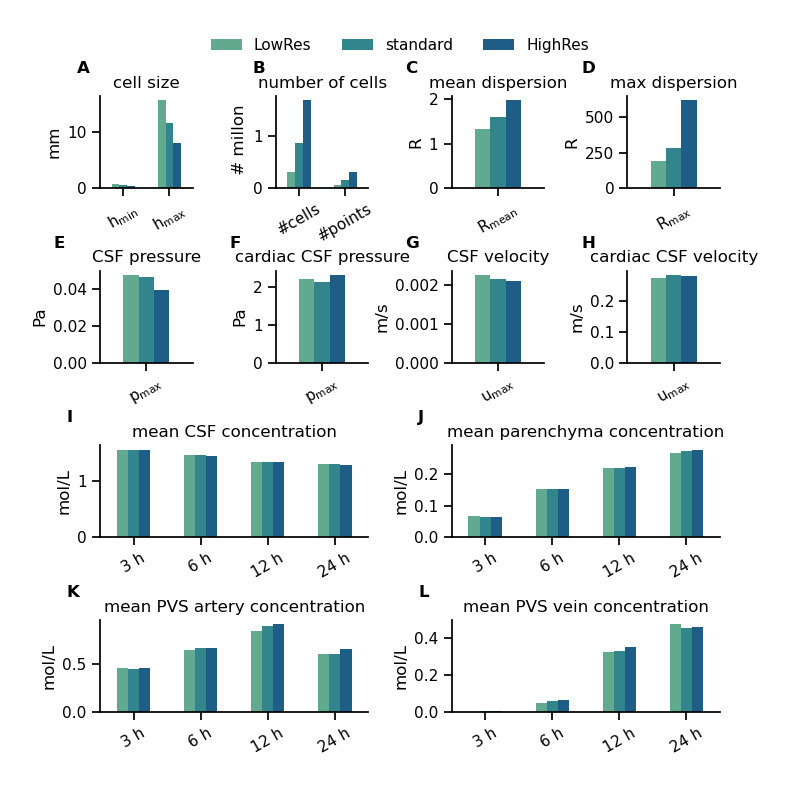
\includegraphics[width=0.9\linewidth]{figures/mesh_refinement.png}
    \caption{Illustration of the three different meshes; from left to right: low resolution, standard resolution, high resolution.}
    \label{fig:mesh_refinement}
\end{figure}

\begin{figure}
    \centering
    \begin{subfigure}[b]{0.45\textwidth}
        \centering
        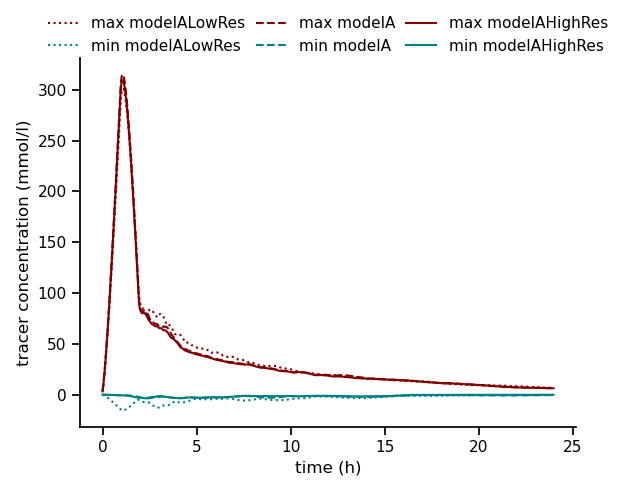
\includegraphics[width = 1 \linewidth]{figures/csf_minmax.png}
        \caption{Minimum and maximum tracer concentration in the CSF under mesh refinement}
    \end{subfigure}
    \begin{subfigure}[b]{0.45\textwidth}
        \centering
     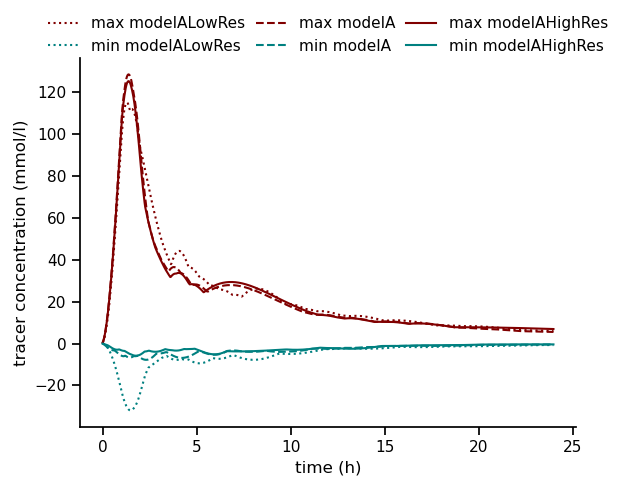
\includegraphics[width= 1 \linewidth]{figures/par_minmax.png}
        \caption{Minimum and maximum tracer concentration in the parenchyma under mesh refinement}
    \end{subfigure}
    \begin{subfigure}[b]{0.45\textwidth}
        \centering
        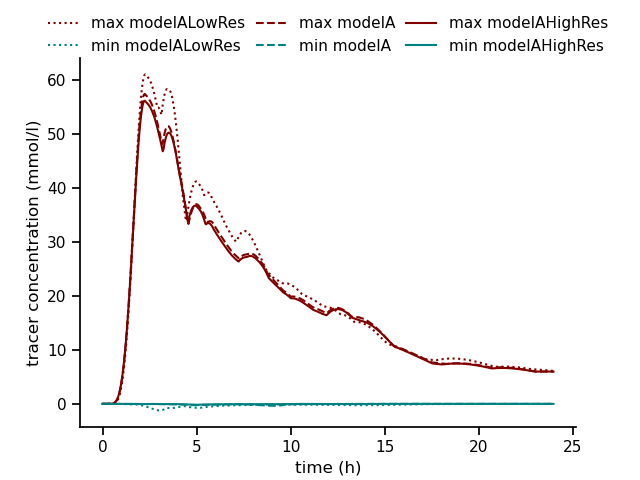
\includegraphics[width = 1 \linewidth]{figures/art_minmax.png}
        \caption{Minimum and maximum tracer concentration in PVSs around arteries under mesh refinement}
    \end{subfigure}
    \begin{subfigure}[b]{0.45\textwidth}
        \centering
     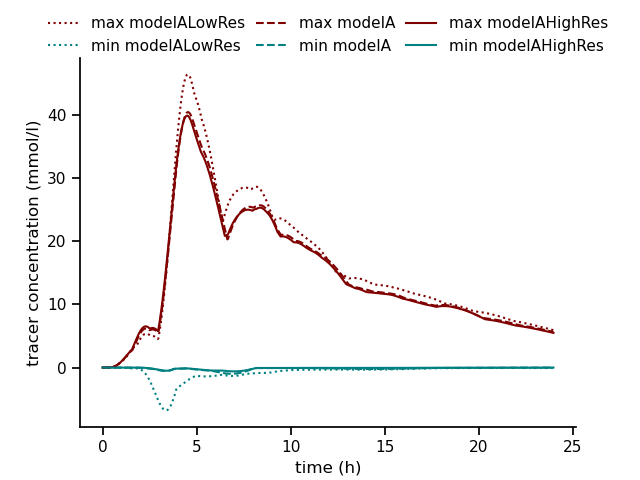
\includegraphics[width= 1 \linewidth]{figures/ven_minmax.png}
         \caption{Minimum and maximum tracer concentration in PVSs around veins under mesh refinement}
    \end{subfigure}
    \caption{Minimum and maximum tracer concentrations over the first 24\,h after injection on the CSF and parenchyma (a), and the arterial and venous PVS (b) computed on the low resolution (LowRes), standard and high resolution (HighRes) meshes with a timestep of 2 min for the baseline model (Model A).}
    \label{fig:mesh_convergence_concentrations}
\end{figure}
\begin{figure}
    \centering
    \begin{subfigure}[b]{0.49\textwidth}
        \centering
        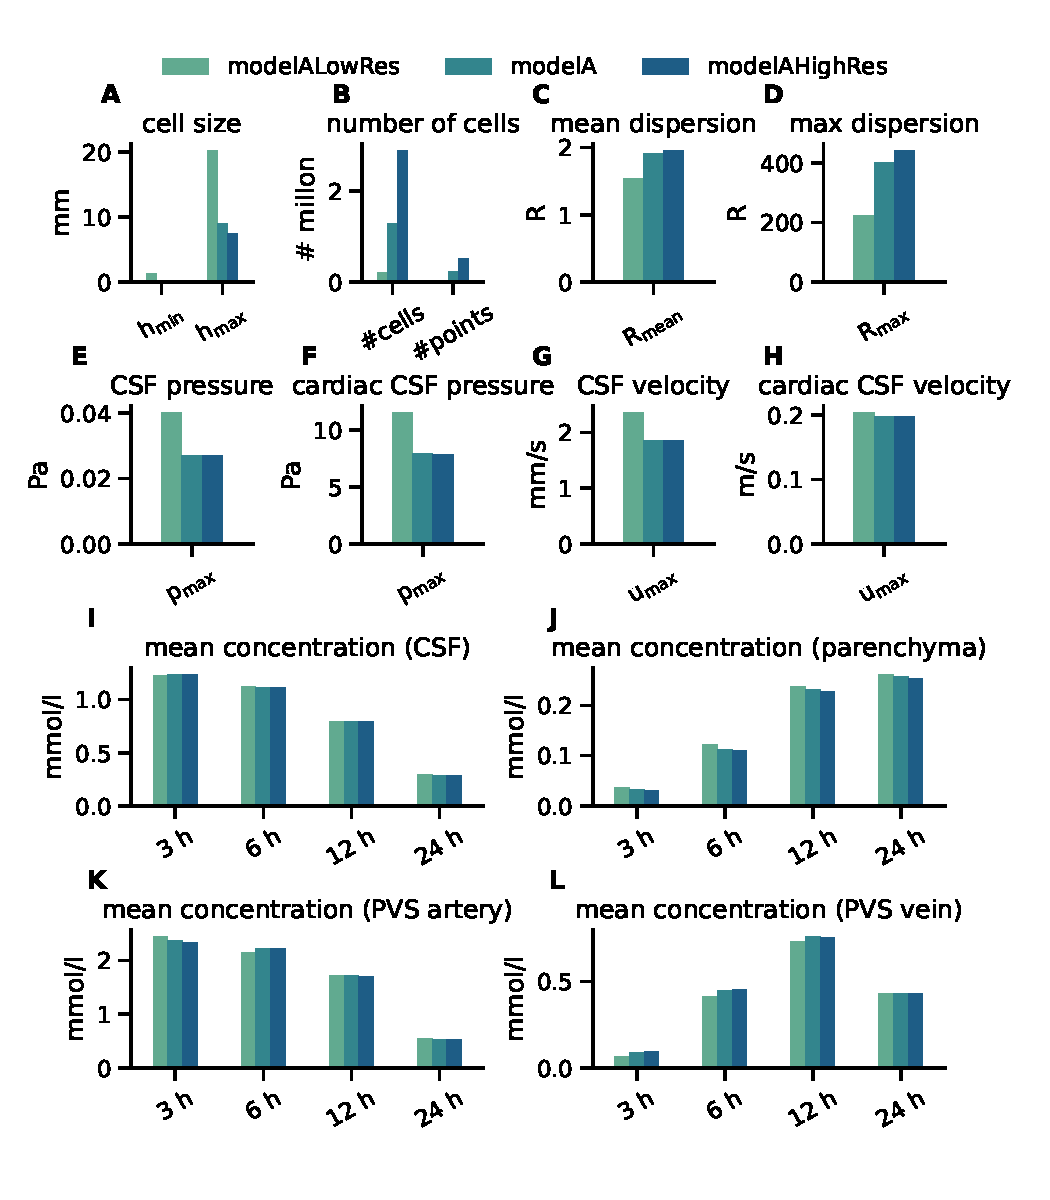
\includegraphics[trim={0.5cm 1cm 0.05cm 0.8cm}, clip, width = 1.05 \linewidth]{figures/modelALowRes_modelA_modelAHighRes.pdf}
        \caption*{Convergence of key quantities of interest with mesh refinement}
        %\label{fig:mesh_convergence}
    \end{subfigure}
    \begin{subfigure}[b]{0.49\textwidth}
        \centering
     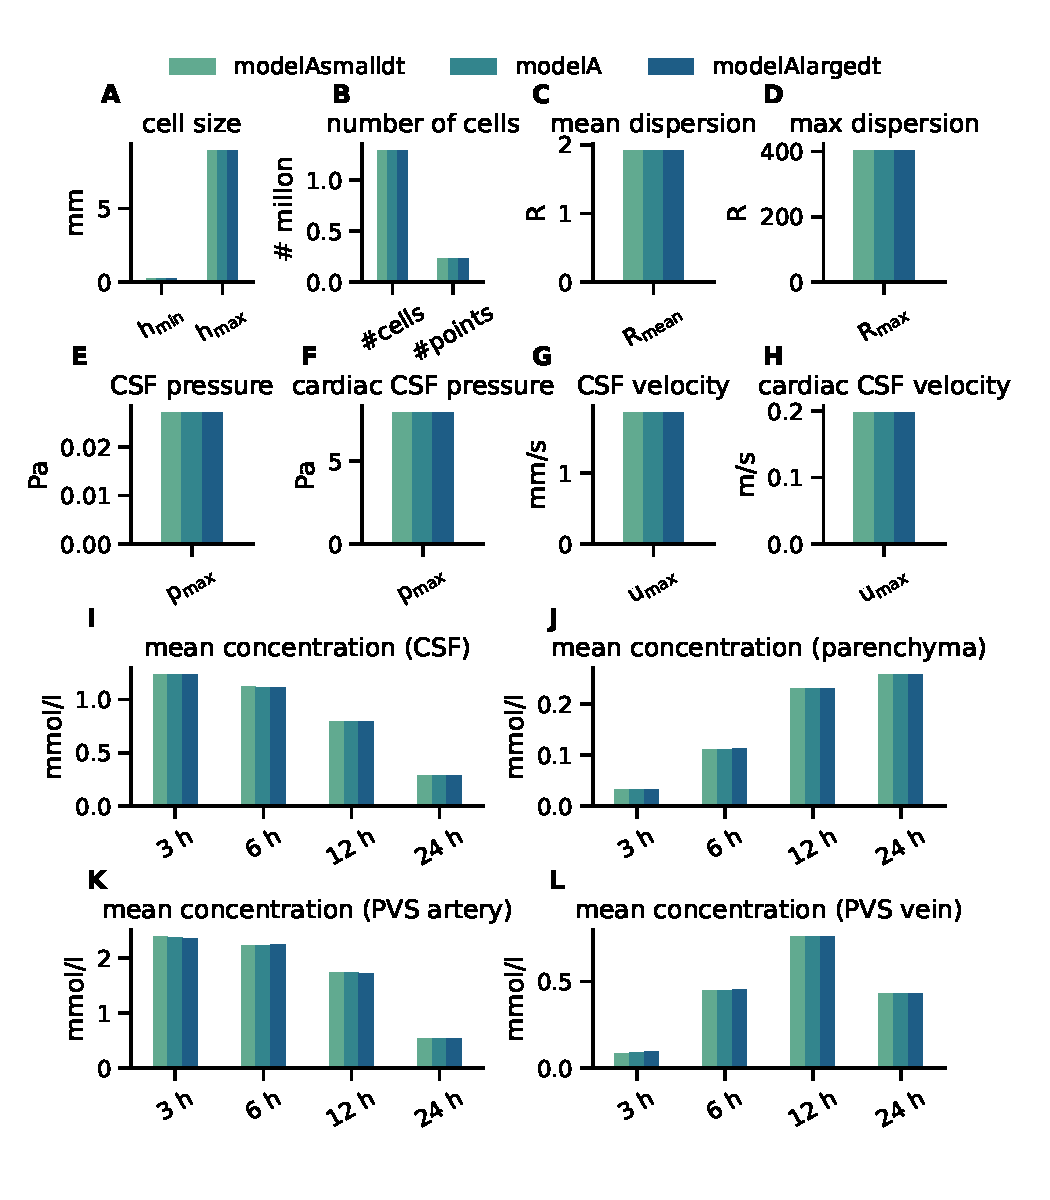
\includegraphics[trim={0.5cm 1cm 0.05cm 0.8cm}, clip,width= 1.05 \linewidth]{figures/modelAsmalldt_modelA_modelAlargedt.pdf}
        \caption*{Convergence of key quantities of interest with time refinement}
        %\label{fig:time_convergence}
    \end{subfigure}
    \caption{For both left and right panels: A: Minimal ($\rm h_{min}$) and maximal ($\rm h_{max}$) mesh cell sizes (computed as cell circumradius $\times 2$); B: number of mesh vertices and tetrahedral cells in each mesh; C: mean cardiac dispersion enhancement factor $R$; D: maximum cardiac dispersion enhancement factor $R$; E: maximum pressure in steady CSF production flow; F: maximum pressure in cardiac-driven CSF flow; G: maximum CSF velocity in steady CSF production flow; H: maximum CSF velocity in cardiac-driven CSF flow; I--L: mean tracer concentration in the CSF, parenchyma, arterial PVS and venous PVS after 3, 6, 12 and 24 hours.}
        \label{fig:mesh_time_convergence}
\end{figure}

\begin{figure}
    \centering
    \begin{subfigure}[b]{0.45\textwidth}
        \centering
        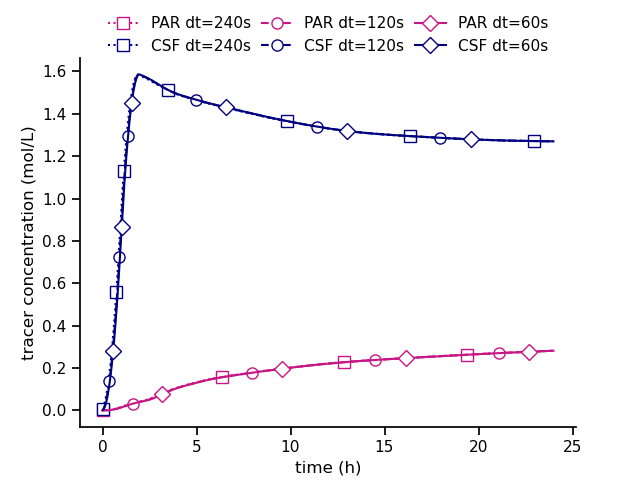
\includegraphics[width = 1 \linewidth]{figures/time_refinement_par_csf_mean.png}
        \caption{Mean tracer concentration in CSF and parenchyma under time step refinement}
    \end{subfigure}
    \begin{subfigure}[b]{0.45\textwidth}
        \centering
     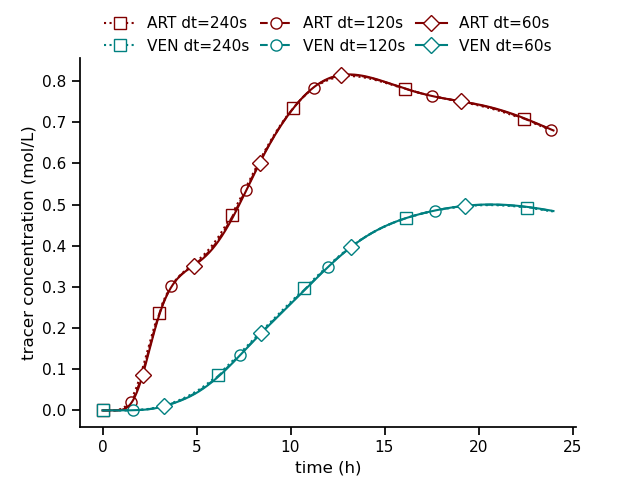
\includegraphics[width= 1\linewidth]{figures/time_refinement_art_ven_mean.png}
         \caption{Mean tracer concentration in PVSs around (veins and) arteries under time step refinement}
    \end{subfigure}
    \caption{Mean tracer concentrations after up to 24\,h in the CSF and parenchyma (a), and the arterial and venous PVS (b) computed on the standard resolution mesh for timesteps of 1, 2, and 4 minutes (dt of 60, 120, or 240 seconds)}
    \label{fig:time_convergence_concentrations}
\end{figure}
\begin{figure}
    \centering
    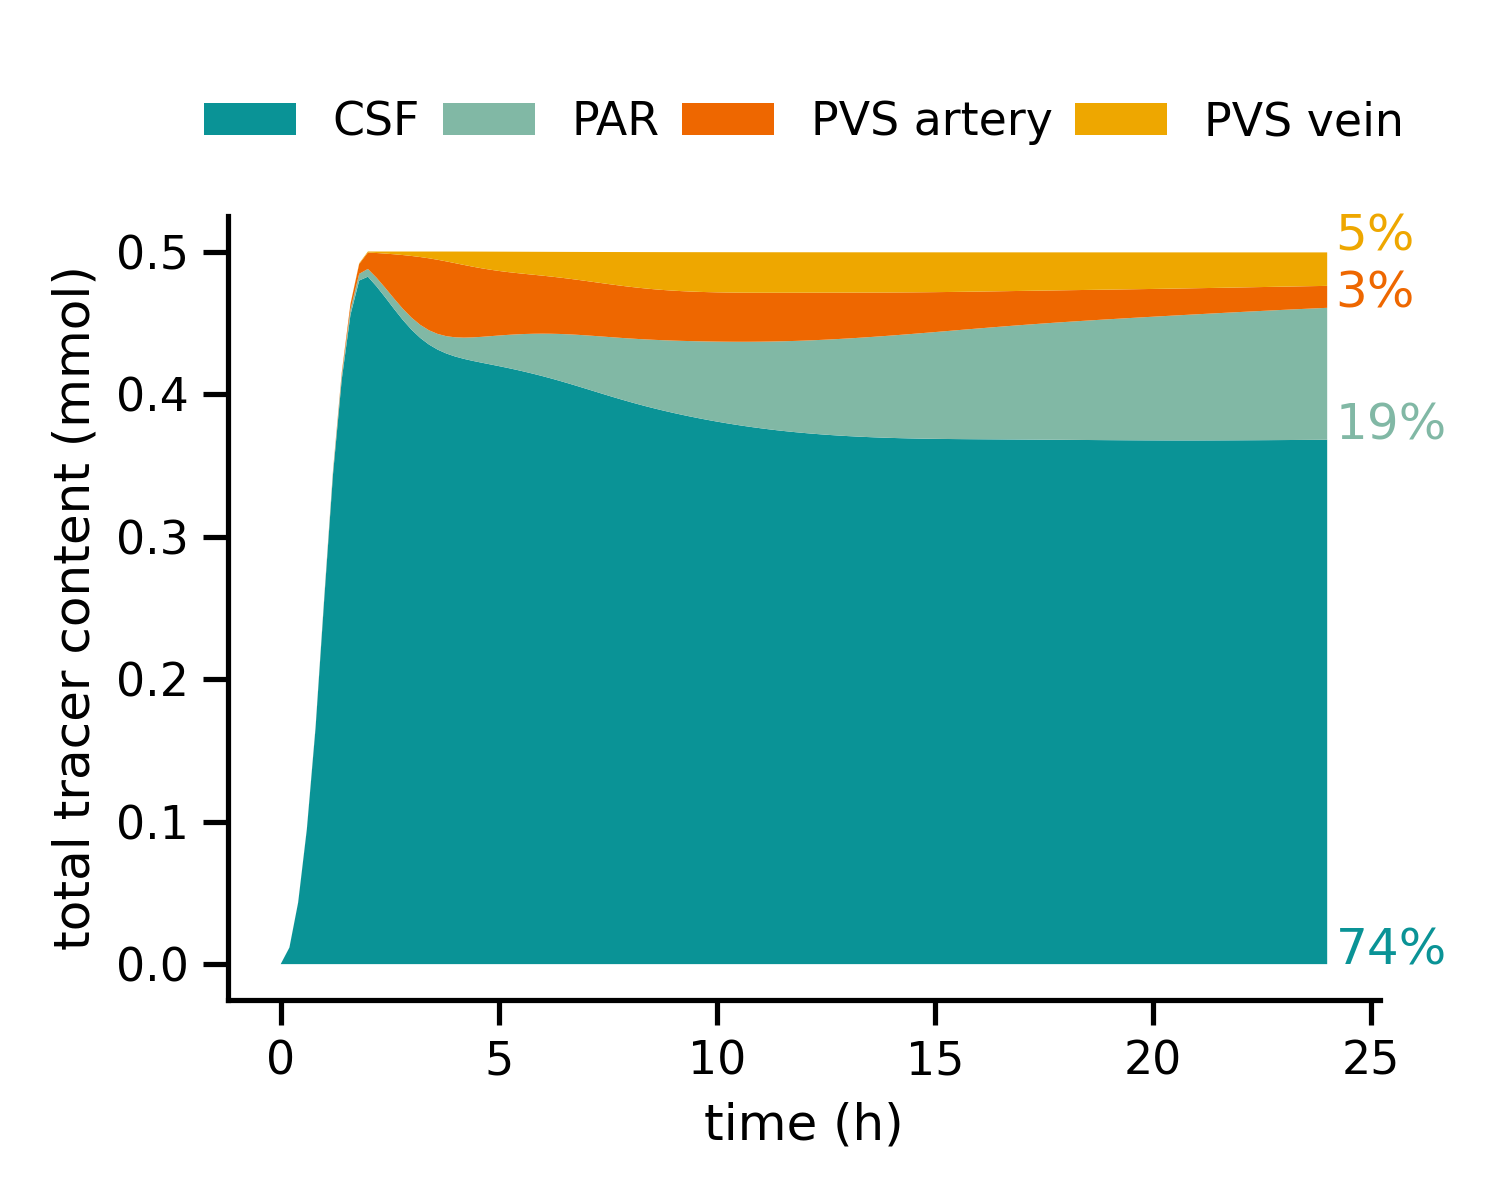
\includegraphics[width=0.5\linewidth]{figures/modelAMassConservation_total_conc.png}
    \caption{Total tracer content in the CSF, parenchyma, and arterial and venous PVS for a variant of the baseline model without tracer outflow. The total amount of tracer is constant after the initial influx phase demonstrating that the numerical scheme conserves mass globally.}
    \label{fig:mass_conservation}
\end{figure}

\section{Supplementary discussion}

\subsection{Extended model validation}
\label{sec:app:model_validation}

In addition to the comparison of our in-silico predictions of tracer
enrichment and clearance against glymphatic MRI, we here compare
auxiliary model quantities against the literature as additional model
validation.

\paragraph{CSF flow and pressures in the SAS and ventricular system}
The dynamics of human CSF flow and pressure are better quantified, by
way of clinical imaging, in-vitro studies, and computational
modelling, in other areas of the ventricular
system~\cite{linninger2007cerebrospinal, sweetman2011cerebrospinal,
  vinje2019respiratory, hornkjol2022csf, causemann2022human,
  karki2025real, liu2025transmantle}. Linninger et
al~\cite{linninger2007cerebrospinal} model CSF flow and pressure
dynamics induced by CSF production and cardiac pulsatility under
normal and hydrocephalic conditions, and report of very good agreement
with Cine (phase-contrast) MRI measurements. Our estimates of the
maximum intracranial pressure difference, 10 Pa from the cardiac
contribution and 26 mPa from CSF production, is in perfect agreement
with their maximum transmantle pressure difference of $\sim$10 Pa, and
also in very good agreement with mean pressure differences of 11.5 Pa
measured clinically between sensors placed subdurally and in the
lateral ventricle \cite{vinje2019respiratory}. Liu et
al~\cite{liu2025transmantle} report of cardiac and respiratory
pressure differences across the aqueduct of 12.1 $\pm$ 5.7 Pa and 9.5
$\pm$ 7.2 Pa, respectively; thus our baseline estimate of the respiratory contribution 1.4 Pa may be an
underestimation. On the other hand, our cardiac- and
respiratory-driven CSF flow estimates peak at 19.8 cm/s and 4.8 cm/s in the caudal direction, respectively, which are higher than phase-contrast MRI measurements of cardiac and respiratory CSF flow
components \cite{takizawa2017characterization, yildiz2017quantifying}. Some variation in CSF flow velocities is expected considering that the values from MRI represent averages
\cite{yildiz2017quantifying} and that the geometry of the CSF spaces
strongly affects peak velocities\cite{vinje2019respiratory,
  causemann2022human}. Hornkjøl et al \cite{hornkjol2022csf} model the
flow dynamics induced by CSF production in the choroid plexus and
report a peak CSF velocity of 8.9 mm/s in the aqueduct, which is 4.8
$\times$ higher than our values of 1.85 mm/s. Given that we use the
same production rate, this deviation again illustrates the impact of
potential differences in the (aqueduct) geometry on local velocities.

% Dispersion predictions
\paragraph{Dispersion in the SAS, ventricular system and PVS}
This pulsatile flow of CSF in the SAS, ventricular system and PVSs
leads to an increase in effective solute
diffusivity~\cite{stockman2007effect, hettiarachchi2011effect,
  asgari2016glymphatic, sharp2019dispersion, ray2021quantitative} via
a process known as Taylor dispersion \cite{taylor1953dispersion,
  watson1983diffusion}. Previous estimates of the magnitude of this
effect in the CSF spaces vary significantly: from an enhancement
factor of 0.05--1 in periarterial spaces surrounding penetrating
arteries~\cite{asgari2016glymphatic, troyetsky2021dispersion}, to
5--100 in the spinal subarachnoid space~\cite{stockman2007effect,
  hettiarachchi2011effect, sharp2019dispersion}, and up to more than
$10\,000$ in surface periarterial spaces~\cite{ray2021quantitative,
  sharp2019dispersion}. The large variability can (at least partly) be
attributed to methodological differences; e.g. different assumptions
on the medium, domain width, pressure differences and/or fluid
velocities, the diversity of CSF flow characteristics, as well as a
high likelihood of spatial variations. Hornkjøl et
al~\cite{hornkjol2022csf} consider model variations with constant
dispersion factors from 1 up to 1000, and indicate that a value of 10
gives the better agreement with the clinically observed
enrichment. Our spatially-varying estimates of the dispersion
enhancement factors $R_c, R_r$ (with $D = (1 + R_c + R_r) D^{\rm
  Gad}$) range from 0 to 200 for the cardiac contribution $R_c$ and 0
to 320 for the respiratory contribution $R_r$; and is thus compatible
within the previously reported spectrum.

% Effect of PVS size and shapes
\paragraph{Shapes, sizes and structures of the PVS}
The shapes, sizes and structures of the PVSs likely vary between
species (e.g.~mice vs.~humans), between spatial compartments
(e.g.~surface vs.~parenchymal), between vessel types (arteries
vs.~arterioles vs.~veins), and in
pathologies~\cite{ichimura1991distribution, foley2012realtime,
  schain2017cortical, mestre2018flow, bedussi2018paravascular,
  mestre2022periarteriolar, smets2024perivascular, raicevic2023sizes,
  vinje2021brain, eide2024functional}. In terms of shape, the PVSs are
commonly represented as annular (elliptic) cylinders, though it is
well recognized that this represents an
idealization~\cite{mestre2018flow, tithof2019hydraulic,
  vinje2021brain, raicevic2023sizes, boster2024hydraulic,
  smets2024perivascular}. In terms of sizes, Raicevic et
al~\cite{raicevic2023sizes} note that the variation in PVS area is
larger between PVS segments than along a single PVS segment and that
the PVS area increases with lumen area. In mice, reports of the ratio
between PVS and lumen area range from
$\approx$0.35--0.43~\cite{smets2024perivascular} up to
$\approx$1.12--1.4~\cite{raicevic2023sizes, mestre2018flow}. In
humans, the PVS may be as wide as the associated surface artery and up
to 4$\times$ wider in iNPH subjects~\cite{eide2024functional}, which
would correspond to substantially larger PVS area ratios (3 or
higher). To reflect the human scale, we here represent each PVS
segment as an annular cylinder with inner radius $R_1$ and outer
radius $R_2$ of width and area proportional to that of the
corresponding blood vessel ($R_2 = 2 R_1$ at baseline, $R_2 = 3 R_1$
for enlarged PVS). The hydraulic resistance of annular cross-sections
is $1-6 \times$~\cite{tithof2019hydraulic} larger than more elongated
cross-sections and thus our estimates of the pressure-induced PVS
velocities are conservative.

%\paragraph{Predictions on overall tracer spreading patterns}

%We compare our in-silico predictions with clinical data from human subjects, in particular the studies by Ringstad et al~\cite{ringstad2018brain}, Watts et al~\cite{watts2019measuring} and Eide and Ringstad~\cite{eide2024functional}. Finding an overall good agreement, we provide a detailed overview on key quantities of interest in %FTA in MCA2 & N/A & N/A & 53.1 ± 50.5 min & 2:12 / 1:48 hours +$t_{st}$ \\
%FTA in ACA2 & N/A & N/A & 48.3 ± 46.1 min & 3:00 hours +$t_{st}$ \\
%\bottomrule
%\end{tabular}
%\caption{Comparison of clinical studies and model predictions on tracer spreading patterns %and arrival times.}
%\label{tab:spreading_comparison}
%\end{table}


\end{document}
